% !TeX program = pdflatex
% Валидация программы измерения зерна ячменя по фотографиям.
% Компилировать из каталога results: pdflatex main.tex (дважды).
\documentclass[12pt,a4paper]{article}

\usepackage[T2A]{fontenc}
\usepackage[utf8]{inputenc}
\usepackage{lmodern}
\usepackage[russian]{babel}
\usepackage{amsmath,amssymb}
\usepackage{graphicx}
\usepackage{pdflscape}
\usepackage{booktabs}
\usepackage{longtable}
\usepackage{siunitx}
\usepackage{geometry}
\usepackage{caption}
\usepackage{float}
\usepackage{array}
\usepackage{enumitem}
\usepackage{indentfirst}
\usepackage[hidelinks]{hyperref}

\geometry{left=2.5cm,right=2.5cm,top=2.5cm,bottom=2.5cm}
\setlength{\emergencystretch}{3em}
\sisetup{
  output-decimal-marker={,},
  group-separator={\,},
  group-digits=integer,
  group-minimum-digits=4,
  detect-all
}
\captionsetup{font=small,labelfont=bf,skip=6pt}
\setlength{\parindent}{1.25cm}
\setlength{\parskip}{0.25em}
\renewcommand{\arraystretch}{1.15}

\title{Валидация программы автоматического измерения размеров зерна ячменя
по восьми фотографиям одной навески}
\author{}
\date{11 ноября 2026 г.}

\newcommand{\LenBias}{$+\num{0.342}$}
\newcommand{\LenBiasLo}{\num{0.325}}
\newcommand{\LenBiasHi}{\num{0.359}}
\newcommand{\LenMae}{\num{0.343}}
\newcommand{\LenRmse}{\num{0.377}}
\newcommand{\LenR}{\num{0.953}}
\newcommand{\LenCcc}{\num{0.781}}
\newcommand{\LenSlope}{\num{0.956}}
\newcommand{\LenIntercept}{+\num{0.718}}
\newcommand{\LenLoaLo}{+\num{0.032}}
\newcommand{\LenLoaHi}{+\num{0.652}}
\newcommand{\LenRatio}{\num{1.0401}}
\newcommand{\LenBiasPct}{\num{4.0}}
\newcommand{\WidBias}{$-\num{0.785}$}
\newcommand{\WidBiasLo}{\num{-0.803}}
\newcommand{\WidBiasHi}{\num{-0.768}}
\newcommand{\WidMae}{\num{0.785}}
\newcommand{\WidRmse}{\num{0.802}}
\newcommand{\WidR}{\num{0.636}}
\newcommand{\WidCcc}{\num{0.063}}
\newcommand{\WidSlope}{\num{0.510}}
\newcommand{\WidIntercept}{+\num{1.011}}
\newcommand{\WidLoaLo}{-\num{1.105}}
\newcommand{\WidLoaHi}{-\num{0.466}}
\newcommand{\WidRatio}{\num{0.7865}}
\newcommand{\WidBiasPct}{\num{21.4}}
\newcommand{\RatioPi}{\num{0.598}}
\newcommand{\RatioMean}{\num{0.7865}}
\newcommand{\RatioLo}{\num{0.7823}}
\newcommand{\RatioHi}{\num{0.7907}}
\newcommand{\PiPred}{\num{2.8781}}
\newcommand{\PiActual}{\num{2.8791}}
\newcommand{\LenSw}{\num{0.246}}
\newcommand{\LenIcc}{\num{0.811}}
\newcommand{\LenIccLo}{\num{0.775}}
\newcommand{\LenIccHi}{\num{0.838}}
\newcommand{\LenRc}{\num{0.681}}
\newcommand{\WidSw}{\num{0.097}}
\newcommand{\WidIcc}{\num{0.738}}
\newcommand{\WidIccLo}{\num{0.700}}
\newcommand{\WidIccHi}{\num{0.770}}
\newcommand{\WidRc}{\num{0.267}}
\newcommand{\CalMean}{\num{-0.305}}
\newcommand{\CalSd}{\num{1.064}}
\newcommand{\CalMin}{\num{-2.095}}
\newcommand{\CalMax}{\num{1.209}}
\newcommand{\CalT}{\num{-0.81}}
\newcommand{\CalP}{\num{0.444}}

\newcommand{\LenMedianBias}{+\num{0.332}}
\newcommand{\LenIqr}{\num{0.174}}
\newcommand{\LenTrimTen}{\num{0.335}}
\newcommand{\LenMape}{\num{4.0}}
\newcommand{\LenSpearman}{\num{-0.119}}
\newcommand{\LenCleanBias}{+\num{0.333}}
\newcommand{\LenCleanMae}{\num{0.335}}
\newcommand{\LenCleanN}{319}
\newcommand{\WidMedianBias}{-\num{0.791}}
\newcommand{\WidIqr}{\num{0.199}}
\newcommand{\WidTrimTen}{\num{-0.791}}
\newcommand{\WidMape}{\num{21.3}}
\newcommand{\WidSpearman}{\num{-0.583}}
\newcommand{\WidCleanBias}{-\num{0.783}}
\newcommand{\WidCleanMae}{\num{0.783}}
\newcommand{\WidCleanN}{321}


\begin{document}
\maketitle

\begin{abstract}
\noindent
Проверена разработанная автором программа пакетной обработки фотографий
зерна ячменя: сегментация зёрен, автоматическая калибровка по линейке и
измерение длины и ширины. Материал — восемь фотографий одной навески из
325 зёрен (13 рядов по 25 зёрен), уложенных вручную; эталон — ручные
измерения штангенциркулем, содержащие 324 заполненные строки (одно зерно
без замера). Программа запускалась без изменения параметров и без подгонки
под эталон. Сегментация нашла все 325 зёрен на каждом снимке без ошибок
сопоставления; повторный прогон дал побитово одинаковый результат.
Масштаб совпал с независимой оценкой по штрихам линейки в пределах
\num{-2.1}\ldots\num{+1.2}\,\% (среднее \CalMean\,\%, СКО \CalSd\,\%).
Длина: смещение $+\num{0.342}$\,мм, MAE \num{0.343}\,мм, $r = \num{0.953}$,
CCC \num{0.781}; ширина: смещение $-\num{0.785}$\,мм, MAE \num{0.785}\,мм,
$r = \num{0.636}$, CCC \num{0.063}. Отношение ширин
«программа/ручной замер» составило \WidRatio, что статистически не
отличается от $\pi/4$ ($p = \RatioPi$): программа измеряет среднюю хорду
(площадь контура, делённая на длину), а ручной замер — максимальную ширину.
Повторяемость по восьми снимкам: ICC(1,1) длины \num{0.811}, ширины
\num{0.738}. Длина пригодна для ранжирования, но абсолютные значения не
взаимозаменяемы; ширина в текущем виде несопоставима со
штангенциркулем по определению. Обобщение ограничено
целыми зёрнами данной навески и данной постановкой съёмки. Приведены
полные таблицы, журнал прогонов, исключения и сведения об отсутствующем
замере.
\end{abstract}

\noindent\textbf{Ключевые слова:} ячмень, зерно, длина, ширина,
обработка изображений, валидация, согласие методов, Блэнд--Альтман,
повторяемость, ICC, калибровка по линейке.

\section{Введение}

Размер и форма зерна — практически значимые признаки. Они связаны с
крупностью и выравненностью семенного материала, с массой 1000 зёрен, с
качеством солода и с технологическими свойствами сырья
\cite{symons1988,tanabata2012}. Поэтому длину, ширину, толщину и массу
зерна регулярно измеряют в селекционных и технологических программах.
Классический инструмент — штангенциркуль; он даёт понятные абсолютные
величины, но требует ручной укладки, не защищён от межоператорских
различий и плохо масштабируется на тысячи зёрен. Фотографическая
морфометрия обещает снять эти ограничения: изображение фиксирует всю
навеску целиком, а измерения выполняются алгоритмом
\cite{li2014,igathinathane2008,sankaran2016,gao2017}.

Известные инструменты анализа изображений семян — например, SmartGrain
\cite{tanabata2012} — показывают, что задача автоматического получения
размеров в принципе решается надёжно. Однако публикации такого рода чаще
демонстрируют возможности метода на новых данных, чем проверяют уже
готовую программу на том же материале, который измерялся вручную, и с
сохранением всех её «боевых» настроек. Между тем именно такая проверка
нужна, если программа уже используется: важно узнать не «может ли
алгоритм измерять», а «совпадают ли его числа с эталонными и в каких
границах этому совпадению можно верить».

Настоящая работа — отчёт о валидации разработанной мной программы
пакетной обработки фотографий зерна. Материалом послужили восемь
фотографий одной навески ячменя (325 зёрен), для которой имеется файл
ручных измерений. Я намеренно не менял ни один параметр сегментации,
калибровки или измерения: проверялось то поведение программы, которое
существует сейчас. Такой выбор имеет цену — часть обнаруженных
расхождений объясняется не ошибками сегментации, а определением
измеряемой величины, и это тоже часть результата. Никакие наблюдения не
удалялись молча: выбросы, «неудобные» снимки и отсутствующий замер
описаны отдельно.

Цель работы — количественно охарактеризовать согласие программы с ручным
измерением по длине и ширине, оценить повторяемость между снимками,
проверить устойчивость калибровки и выявить режимы, в которых программа
работает хуже. В задачи входило: (1) прогнать все восемь снимков одной
версией программы и сохранить журнал; (2) установить однозначное
соответствие между зёрнами на фотографиях и строками ручного файла;
(3) рассчитать смещение, MAE, RMSE, корреляцию, коэффициент согласия
Лин и пределы согласия Блэнда--Альтмана; (4) разделить изменчивость
между зёрнами и между снимками; (5) проверить, чем объясняется
расхождение по ширине; (6) перечислить допущения и открытые вопросы.

Работа ограничена целыми зёрнами одной навески, снятыми в одной серии.
Толщина и масса программой в пакетном режиме не экспортируются, поэтому
они не валидируются; выводы о них не делаются. Вопросы влажности,
влияния освещения и межоператорской воспроизводимости ручных замеров
обсуждаются как ограничения, а не как измеренные факторы.

\section{Материалы и методы}

\subsection{Материал и снимки}

Материал — одна навеска ячменя из 325 зёрен, уложенных оператором на
тёмный фон в 13 рядов по 25 зёрен (ряды и позиции в ряду заданы
физически). Сведения о происхождении образца, сорте, влажности и условиях
хранения мне не предоставлены. Все восемь фотографий сделаны, по
словам оператора, с одной навески. Серия включает снимки без суффикса
\texttt{p} (далее non-P) и с суффиксом \texttt{p} (далее P). На
P-снимках зерно, судя по изображениям, лежит бороздкой вверх; на
non-P признак бороздки в основном не обнаруживается. Это означает, что
ориентация зёрен между кадрами менялась, хотя состав навески, по
утверждению оператора, оставался одним и тем же. Оператор также указал три снимка «лучшего фокуса»: \texttt{1\_2},
\texttt{2\_1} и \texttt{2\_1p}. Эти три утверждения — заявления
оператора; независимо я их не проверял и далее обозначаю как заявленные.
Влажность зерна не измерялась, температура и освещение не
документированы, параметры камеры в отчёте не фиксировались.

Файлы изображений: \texttt{1\_1}, \texttt{1\_2}, \texttt{1\_3},
\texttt{2\_1}, \texttt{2\_1p}, \texttt{2\_2}, \texttt{2\_2p},
\texttt{2\_3p}. Размеры кадров — примерно \num{4500}--\num{5000}~px по
ширине и \num{3064}~px по высоте. В нижней части каждого кадра видна
металлическая линейка с сантиметровыми и миллиметровыми штрихами; она
используется программой для калибровки. Зёрна на снимках не касаются
друг друга, что важно: программа проверялась на ситуации
«неперекрывающиеся целые зёрна», а не на слипшихся объектах.

\subsection{Ручной эталон}

Ручной файл \texttt{Ruchnye\_zamery\_zerna\_po\_ryadam.xlsx} содержит
325 строк (13 рядов по 25 позиций) и столбцы длины, ширины, толщины и
массы. Заполнены 324 строки; в ряду~11, позиция~25 (серийный номер 275)
стоит прочерк. Оператор сообщил, что измерения выполнены
штангенциркулем, а значения округлялись до \num{0.1}\,мм. Последнее
утверждение на данных не подтверждается: около \num{99}\,\% значений
длины и ширины лежат на сетке \num{0.05}\,мм, а на сетке \num{0.1}\,мм —
лишь \num{52.8} и \num{49.7}\,\% соответственно (табл.~\ref{tab:manual}).
Иными словами, фактический шаг записи — \num{0.05}\,мм, и примерно
половина значений имеет нечётный шаг \num{0.05}\,мм. Природа ручного
протокола (какая именно ширина и длина измерялись, сколько раз, одним ли
оператором) в файле не задокументирована; я принимаю ручные значения как
эталон, но учитываю это как источник неопределённости.

\begin{table}[htbp]
\centering\footnotesize
\setlength{\tabcolsep}{3pt}
\caption{Сводка ручных измерений (число заполненных строк $n = 324$;
длина, ширина и толщина — в мм, масса — в г).}
\label{tab:manual}
\begin{tabular}{@{}lrrrrrrr@{}}
\toprule
Признак & $n$ & \shortstack{Среднее\\$\pm$ СКО} & Медиана & Мин--макс &
\shortstack{Уникальных\\значений} & \shortstack{На сетке\\0,05, \%} &
\shortstack{На сетке\\0,1, \%} \\
\midrule
Длина & 324 & $\num{8.595} \pm \num{0.515}$ & \num{8.600} & \num{7.200}--\num{9.800} & 55 & \num{99.1} & \num{52.8} \\
Ширина & 324 & $\num{3.665} \pm \num{0.207}$ & \num{3.650} & \num{2.900}--\num{4.450} & 29 & \num{98.8} & \num{49.7} \\
Толщина & 324 & $\num{2.785} \pm \num{0.147}$ & \num{2.800} & \num{2.200}--\num{3.250} & 21 & \num{99.1} & \num{57.4} \\
Масса & 324 & $\num{0.050} \pm \num{0.020}$ & \num{0.049} & \num{0.028}--\num{0.298} & 238 & \num{0.3} & \num{0.0} \\
\bottomrule
\end{tabular}

\end{table}

Кроме того, в ручном файле есть два явных выброса по массе: зерно 162
(ряд~7, позиция~12) — \num{0.29765}\,г и зерно 310 (ряд~13,
позиция~10) — \num{0.29195}\,г, что примерно в шесть раз больше медианы
(\num{0.0488}\,г). Робастные $z$-оценки равны \num{35.1} и \num{34.3}.
Масса в настоящей валидации не используется, поскольку программа её в
пакетном режиме не выдаёт; эти значения важны лишь для оценки массы
1000 зёрен (по всем строкам \num{50.02}\,г, без двух выбросов
\num{48.50}\,г) и как признак возможных ошибок записи. Причину выбросов
я не установил.

\subsection{Программа}

Проверялась разработанная мной программа на Python (OpenCV,
scikit-image, NumPy, SciPy \cite{bradski2000,vanderwalt2014,harris2020,virtanen2020}).
Пакетный режим запускается командой для каждого файла изображения и
обрабатывает кадр целиком. Параметры не менялись и соответствовали
значениям по умолчанию: размытие 21~px, морфологические ядра 2 и 5~px,
минимальная площадь \num{3000}\,px, максимальная \num{40000}\,px,
минимальная вытянутость 1{,}0, максимальная 4{,}5, минимальная
solidity 0{,}60, минимальный extent 0{,}30, порог ширины границы для
«сфокусированного» \num{3.9}\,px, для «размытого» \num{6.0}\,px.
Порог признака бороздки \num{11.0} (score) также не менялся.

Сегментация выделяет зёрна как светлые объекты на тёмном фоне с
фильтрацией по площади, вытянутости, solidity и extent. Я проверял
результат не только по числу объектов, но и по структуре укладки:
восстановленные центры зёрен образуют 13 рядов по 25 объектов, а
расстояние до ближайшего соседа внутри ряда составляет
\num{103}--\num{118}\,px (медиана \num{128}--\num{146}\,px); ошибок
сопоставления «ряд--позиция» не обнаружено. Дополнительно каждый
обработанный фрагмент сохраняется в виде контура, что позволяет
пересчитать геометрию независимо от программы.

Длина в программе — длина самого длинного внутреннего хордового отрезка
между наиболее удалёнными точками контура (с поиском внутренней хорды,
если диаметр выходит за контур). Ширина вычисляется как
\begin{equation}
W_{\text{прог}} = \min\!\left(\frac{A_{\text{hull}}}{L},\; w_{\text{rect}}\right),
\label{eq:width}
\end{equation}
где $A_{\text{hull}}$ — площадь выпуклой оболочки контура, $L$ — длина,
$w_{\text{rect}}$ — короткая сторона минимального повёрнутого
прямоугольника. На всех \num{2600} наблюдениях победила первая ветвь:
$A_{\text{hull}}/L$ оказалась меньше $w_{\text{rect}}$ (проверка
независимым пересчётом: максимальное расхождение экспортированной ширины
с $\min(A_{\text{hull}}/L, w_{\text{rect}})$ не превысило
\num{0.0005}\,px). Следовательно, экспортируемая ширина — это средняя
хорда (площадь, делённая на длину), а не максимальная ширина. Для
эллипса $A = \pi ab$, $L = 2a$, полная ширина $W = 2b$, поэтому
$A/L = \pi W/4 \approx \num{0.785}\,W$. Это соотношение проверяется в
разделе результатов; деталь существенна для интерпретации расхождений.

Калибровка масштаба выполняется по линейке в кадре: программа ищет
линейку, детектирует штрихи и оценивает шаг. В текущей версии после
оценки сантиметрового масштаба стоит безусловное умножение на 2 с
комментарием в коде о предполагаемом пропуске половины штрихов; это
недокументированное допущение, и оно проверяется отдельно. Размеры в
миллиметрах получаются умножением пиксельных величин на автоматически
найденный \texttt{mm\_per\_px}. В экспортируемом CSV для пакетного режима
есть поля \texttt{file\_index}, \texttt{index}, \texttt{status},
\texttt{color\_hex}, \texttt{edge\_width\_px}, \texttt{length\_px},
\texttt{width\_px}, \texttt{angle\_deg}, \texttt{area\_px},
\texttt{has\_groove} и \texttt{mm\_per\_px}. Толщины, массы и объёма в
файле нет; я не достраивал их из пикселей.

\subsection{Сопоставление данных}

Программа нумерует сохранённые фрагменты последовательно, и для каждого
снимка формируется \texttt{file\_index} вида
\texttt{<снимок>\_<NNN>}, где \texttt{NNN} — номер зерна. Ручной файл
нумерует строки серийно от 1 до 325 в порядке «ряд~1, позиции~1--25,
ряд~2, \ldots». Прямое сопоставление «серийный номер = номер программы»
подтверждается структурой: на всех снимках программа устойчиво находит
13 рядов по 25 зёрен, а проверка сдвигов на рядах 12--13 даёт для прямого
сопоставления $r = \num{0.937}$ и MAE \num{0.407}\,мм, тогда как сдвиг на
$\pm 1$ разрушает корреляцию ($r = \num{0.010}$ и \num{-0.031}). Поэтому
я принял прямое сопоставление. Отсутствие ручного замера именно на
позиции 25 ряда~11 (серийный номер 275) не сдвигает нумерацию: программа
находит на этой позиции зерно на всех восьми снимках (проверено по
координатам, табл.~\ref{tab:missing}). Если бы мапирование строилось по
числу заполненных строк ряда (24 вместо 25), ряды 12--13 сместились бы,
что данным противоречит. Тест «какое $k$ пропущено в ряду 11» по самим
изображениям неоднозначен: минимальная MAE длины достигается при
$k = 19$ (\num{0.366}\,мм), при $k = 25$ MAE равна \num{0.377}\,мм;
разница мала, и я использую $k = 25$ как структурное (25 зёрен в ряду),
а не «оптимальное по эталону» значение. Чувствительность к этому выбору
показана в разделе результатов.

\begin{table}[htbp]
\centering\small
\setlength{\tabcolsep}{4pt}
\caption{Зерно 275 (ряд~11, позиция~25): программа находит его на всех
восьми снимках, но ручного замера для него нет.}
\label{tab:missing}
\begin{tabular}{@{}lrrrrr@{}}
\toprule
Снимок & Индекс & $c_x$, px & $c_y$, px & $b_w \times b_h$, px & NN, px \\
\midrule
1\_1 & 275 & \num{3968.5} & \num{2089.5} & 67x133 & \num{138.0} \\
1\_2 & 275 & \num{3979.0} & \num{2040.0} & 72x138 & \num{142.9} \\
1\_3 & 275 & \num{4304.0} & \num{2147.0} & 78x148 & \num{151.0} \\
2\_1 & 275 & \num{4118.0} & \num{2180.5} & 64x135 & \num{164.5} \\
2\_1p & 275 & \num{4226.5} & \num{2201.5} & 71x143 & \num{189.5} \\
2\_2 & 275 & \num{4308.5} & \num{2244.0} & 69x144 & \num{172.5} \\
2\_2p & 275 & \num{4257.0} & \num{2210.0} & 72x144 & \num{190.6} \\
2\_3p & 275 & \num{3815.5} & \num{2198.5} & 65x131 & \num{172.0} \\
\bottomrule
\end{tabular}

\end{table}

Единица анализа — зерно, а не наблюдение: восемь снимков — это
повторные измерения одного и того же физического зерна. Поэтому
первичные метрики согласия считаются по 324 зёрнам (среднее программы
по восьми снимкам), а вариация между снимками анализируется отдельно
как повторяемость. Такой подход не раздувает $n$ и не выдаёт
внутриснимковую корреляцию за независимую.

\subsection{Статистические методы}

Для каждого признака обозначим ручное значение $M_i$, программное
$P_i$ (среднее по восьми снимкам для зерна $i$), разность
$d_i = P_i - M_i$. Рассчитывались: среднее смещение с 95\,\% доверительным
интервалом (ДИ); MAE; RMSE; коэффициент корреляции Пирсона $r$;
коэффициент согласия Линя (CCC) \cite{lin1989}; линейная регрессия
$P = a + bM$ (программа от ручного значения) с проверкой $b = 1$ и
$a = 0$; отношение $P/M$; пределы согласия Блэнда--Альтмана
$\bar d \pm 1.96\,s_d$ и доля точек внутри них \cite{bland1986}.
ДИ для смещения — по $t$-распределению, для MAE, RMSE и $r$ —
перцентильный бутстрэп (1000 повторностей, зерно генератора
зафиксировано). Дополнительно считались медиана смещения, межквартильный
размах, усечённое на 10\,\% среднее, MAPE, медианная абсолютная ошибка
и коэффициент Спирмена — как робастная проверка того, что выводы не
держатся на нескольких точках.

Повторяемость между снимками оценивалась по матрице «зерно $\times$
снимок» (325 строк, 8 столбцов) через однофакторную модель случайных
эффектов: ICC(1,1) \cite{shrout1979}, внутризерновое СКО
$S_w = \sqrt{\mathrm{MSW}}$ и коэффициент повторяемости
$\mathrm{RC} = 1.96\sqrt{2}\,S_w$. ДИ для ICC — перцентильный бутстрэп по
зернам. Сравнения подгрупп (P против non-P, «заявленный лучший фокус»
против остальных) выполнялись как парные: для каждого зерна сравнивались
средние по соответствующим снимкам, что убирает межзерновую
изменчивость. Для эффекта статуса (focused/transition/blurry)
использовался критерий Краскела--Уоллиса \cite{kruskal1952} на
внутризерновых отклонениях. Выбросы определялись по робастной
$z$-оценке $0.6745\,(d - \mathrm{med})/\mathrm{MAD}$ с порогом $|z| > 3.5$;
они не удалялись, а приводились отдельно и исключались только в анализе
чувствительности.

Все расчёты и рисунки выполнены в Python (NumPy, SciPy, pandas,
matplotlib, OpenCV, scikit-image); проверочные таблицы и полные выгрузки
лежат в каталоге \texttt{results}. Я не подбирал параметры программы по
эталону; единственная величина, которая обсуждалась как «настроенная»,
— порог бороздки \num{11.0}, и он остался тем, что был в коде.

\section{Результаты}

\subsection{Сегментация, журнал и детерминизм}

Все восемь снимков обработаны одной версией программы в один сеанс.
На каждом снимке найдено и сохранено ровно 325 фрагментов; код возврата
равен нулю, время обработки — от \num{4.05} до \num{6.82}\,с
(табл.~\ref{tab:runlog} в приложении~Б). Визуально контуры покрывают все
зёрна, включая краевые; на рис.~\ref{fig:detection} показан пример
разметки. Число объектов совпало с ожидаемым, но я не ограничивался
этим: по координатам центров восстановлена структура 13 рядов по 25
зёрен, расстояния до ближайшего соседа и размеры ограничивающих рамок
приведены в табл.~\ref{tab:segmentation}. Ни в одном снимке не возникло
сдвига ряда или позиции; это важно, потому что при потере одного зерна
программа могла бы «подхватить» соседнее и дать правдоподобные, но
неверные пары.

\begin{figure}[H]
\centering
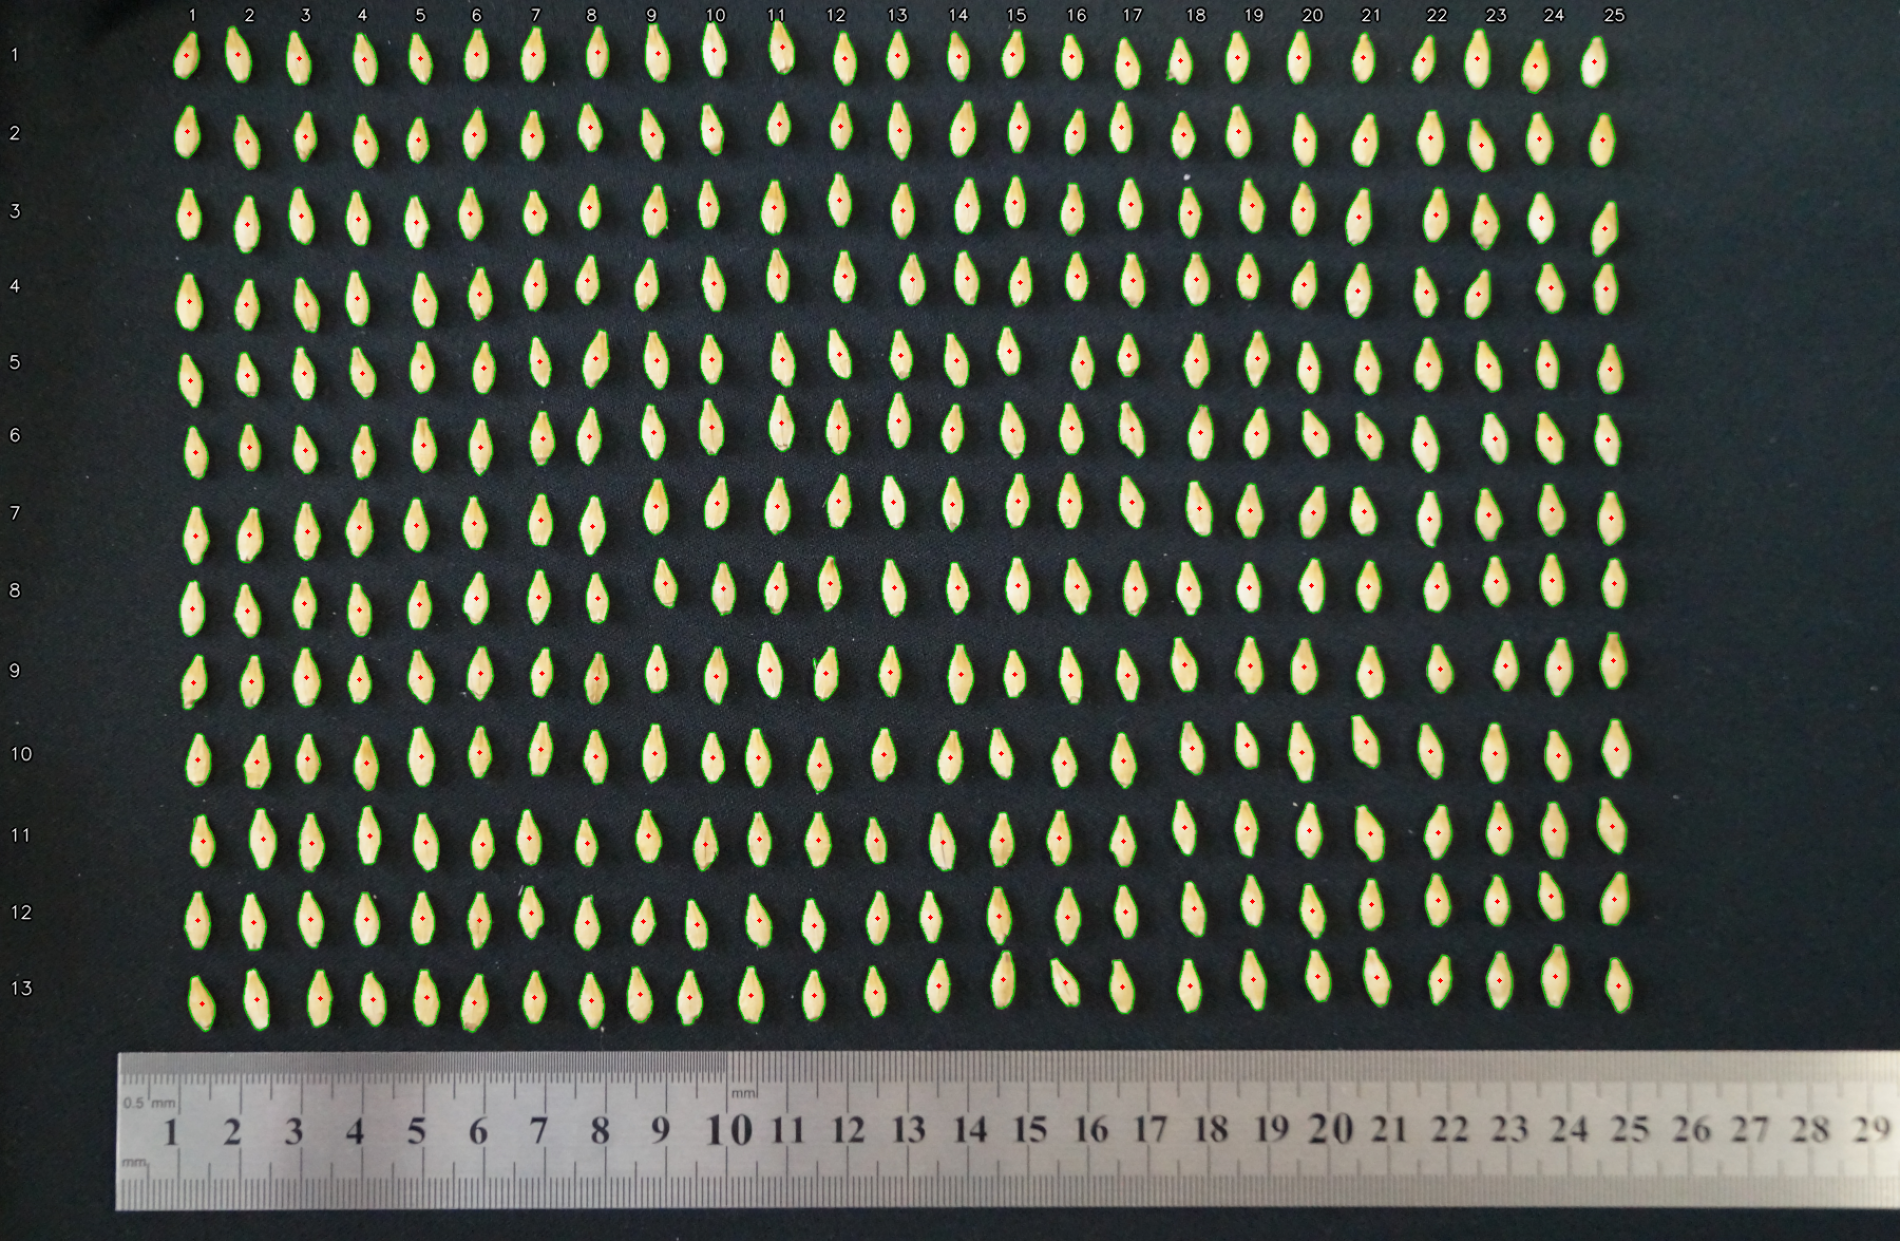
\includegraphics[width=0.85\linewidth]{figures/fig_detection.png}
\caption{Пример результата сегментации: контуры всех 325 зёрен и
автоматически найденные центры. Снимок \texttt{1\_1}; линейка в нижней
части кадра используется для калибровки.}
\label{fig:detection}
\end{figure}

Повторный прогон снимка \texttt{1\_2} дал те же 325 строк; максимальное
абсолютное расхождение числовых полей равно нулю, различий по
\texttt{status}, \texttt{color\_hex} и \texttt{has\_groove} нет
(табл.~\ref{tab:determinism}). Это ожидаемо для детерминированного
алгоритма без случайной инициализации, но проверка важна: она
показывает, что вся наблюдаемая вариация между снимками относится к
изображениям, а не к нестабильности запуска.

\begin{table}[htbp]
\centering\footnotesize
\setlength{\tabcolsep}{3pt}
\caption{Проверка детерминизма: два прогона снимка \texttt{1\_2}.}
\label{tab:determinism}
\begin{tabular}{@{}rrrrrr@{}}
\toprule
\shortstack{Строк\\в 1-м прогоне} & \shortstack{Строк\\во 2-м} &
\shortstack{$\max|\Delta|$\\числовой} & \shortstack{Различий\\status} &
\shortstack{Различий\\color} & \shortstack{Различий\\groove} \\
\midrule
325 & 325 & \num{0.0} & 0 & 0 & 0 \\
\bottomrule
\end{tabular}

\end{table}

\subsection{Калибровка масштаба}

Автоматическая калибровка по линейке дала \texttt{mm\_per\_px} от
\num{0.0632} до \num{0.0708}\,мм/px (табл.~\ref{tab:calibration}).
Независимая оценка по периодичности штрихов линейки (автокорреляция
профиля вдоль линейки, без использования детектора штрихов программы)
дала значения, отличающиеся в среднем на \CalMean\,\% (СКО \CalSd\,\%,
диапазон \CalMin\ldots\CalMax\,\%). Среднее отличие статистически не
отличается от нуля ($t = \CalT$, $p = \CalP$). Наибольшее отклонение —
снимок \texttt{1\_1} (\num{-2.095}\,\%), наименьшее — \texttt{1\_2}
(\num{+0.010}\,\%).

\begin{table}[H]
\centering\small
\caption{Сравнение автоматической калибровки с независимой оценкой по
штрихам линейки.}
\label{tab:calibration}
\begin{tabular}{@{}lrrr@{}}
\toprule
Снимок & Программа, мм/px & Независимая оценка, мм/px & Отличие, \% \\
\midrule
1\_1 & \num{0.068465} & \num{0.069930} & $-\num{2.095}$ \\
1\_2 & \num{0.066822} & \num{0.066815} & $+\num{0.010}$ \\
1\_3 & \num{0.063253} & \num{0.063291} & $-\num{0.060}$ \\
2\_1 & \num{0.066270} & \num{0.067265} & $-\num{1.479}$ \\
2\_1p & \num{0.064464} & \num{0.063694} & $+\num{1.209}$ \\
2\_2 & \num{0.063195} & \num{0.063291} & $-\num{0.152}$ \\
2\_2p & \num{0.063944} & \num{0.063559} & $+\num{0.606}$ \\
2\_3p & \num{0.070832} & \num{0.071174} & $-\num{0.481}$ \\
\bottomrule
\end{tabular}

\end{table}

\begin{figure}[H]
\centering
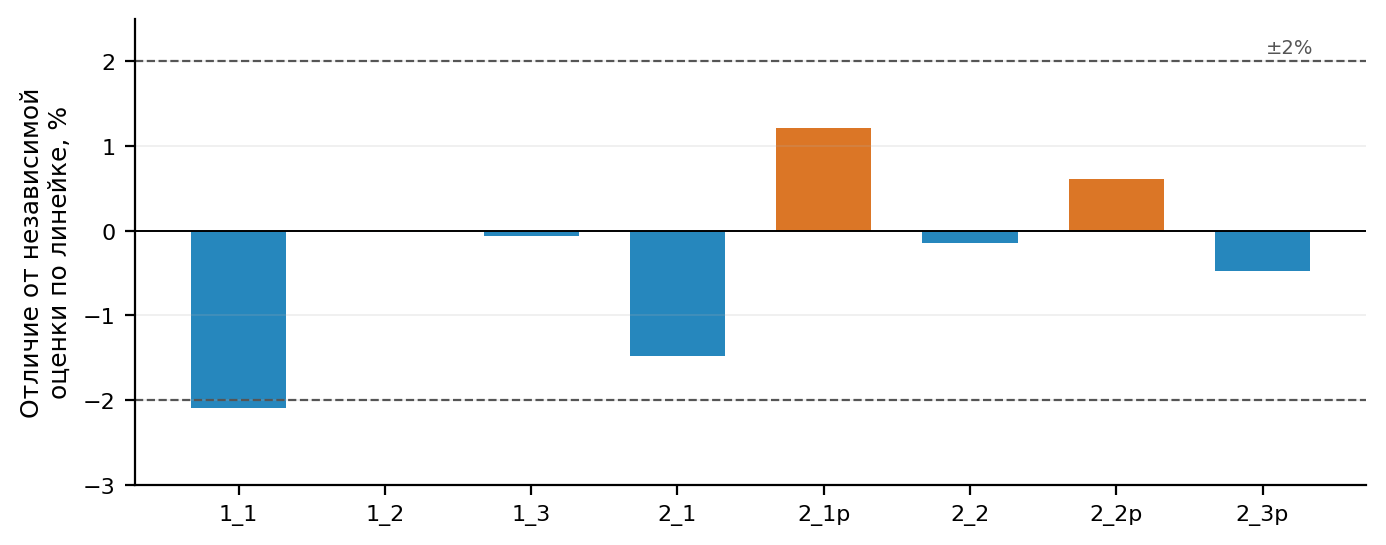
\includegraphics[width=0.70\linewidth]{figures/fig_calibration.png}
\caption{Относительное отличие автоматического масштаба от независимой
оценки по линейке. Пунктир — границы $\pm 2\,\%$.}
\label{fig:calibration}
\end{figure}

Формально калибровка прошла: ошибка масштаба около \num{2}\,\% даёт
примерно \num{0.18}\,мм на длине \num{9}\,мм и \num{0.06}\,мм на ширине
\num{3}\,мм, то есть не может объяснить ни смещение длины
$+\num{0.34}$\,мм, ни смещение ширины $-\num{0.79}$\,мм. Но способ,
которым этот результат получен, хрупок: в коде стоит безусловное
умножение на 2, компенсирующее систематический недодетект штрихов. На
этих восьми снимках с данной линейкой и данным разрешением допущение
сработало; на другой линейке, другом масштабе или другом кадрировании
оно может дать ошибку в два раза. Это не ошибка валидации, а
недокументированный риск программы, и я фиксирую его явно.

\subsection{Длина}

Сводка согласия по длине приведена в табл.~\ref{tab:overall} и на
рис.~\ref{fig:agreement}a,b. Среднее ручное значение — \num{8.595}~мм
(СКО \num{0.515}), среднее программы — \num{8.937}~мм (СКО \num{0.517}).
Смещение программы относительно ручного замера: \LenBias~мм
(95\,\% ДИ \LenBiasLo\ldots\LenBiasHi), то есть программа систематически
завышает длину примерно на \num{4.0}\,\%. MAE равна \LenMae~мм, RMSE —
\LenRmse~мм, корреляция \LenR, CCC \LenCcc. Пределы согласия —
\LenLoaLo\ldots\LenLoaHi~мм; внутри них лежит \num{94.75}\,\% точек. Это
широкие пределы: даже после вычитания среднего смещения отдельное зерно
может отличаться на несколько десятых миллиметра.

\begin{table}[H]
\centering\scriptsize
\setlength{\tabcolsep}{3pt}
\caption{Согласие программы с ручным измерением по всем 324 зёрнам
(среднее программы по восьми снимкам).}
\label{tab:overall}
\begin{tabular}{@{}lrrrrrrrr@{}}
\toprule
Признак & $n$ & \shortstack{Вручную,\\мм} & \shortstack{Программа,\\мм} &
\shortstack{Смещение\\{[95\% ДИ], мм}} &
\shortstack{MAE\\{[95\% ДИ], мм}} & \shortstack{RMSE,\\мм} & $r$ & CCC \\
\midrule
Длина & 324 & $\num{8.595} \pm \num{0.515}$ & $\num{8.937} \pm \num{0.517}$ & $+\num{0.342}$ [\num{0.325}; \num{0.359}] & \num{0.343} [\num{0.327}; \num{0.361}] & \num{0.377} & \num{0.953} & \num{0.781} \\
Ширина & 324 & $\num{3.665} \pm \num{0.207}$ & $\num{2.879} \pm \num{0.166}$ & $-\num{0.785}$ [\num{-0.803}; \num{-0.768}] & \num{0.785} [\num{0.768}; \num{0.803}] & \num{0.802} & \num{0.636} & \num{0.063} \\
\bottomrule
\end{tabular}

\end{table}

\begin{figure}[htbp]
\centering
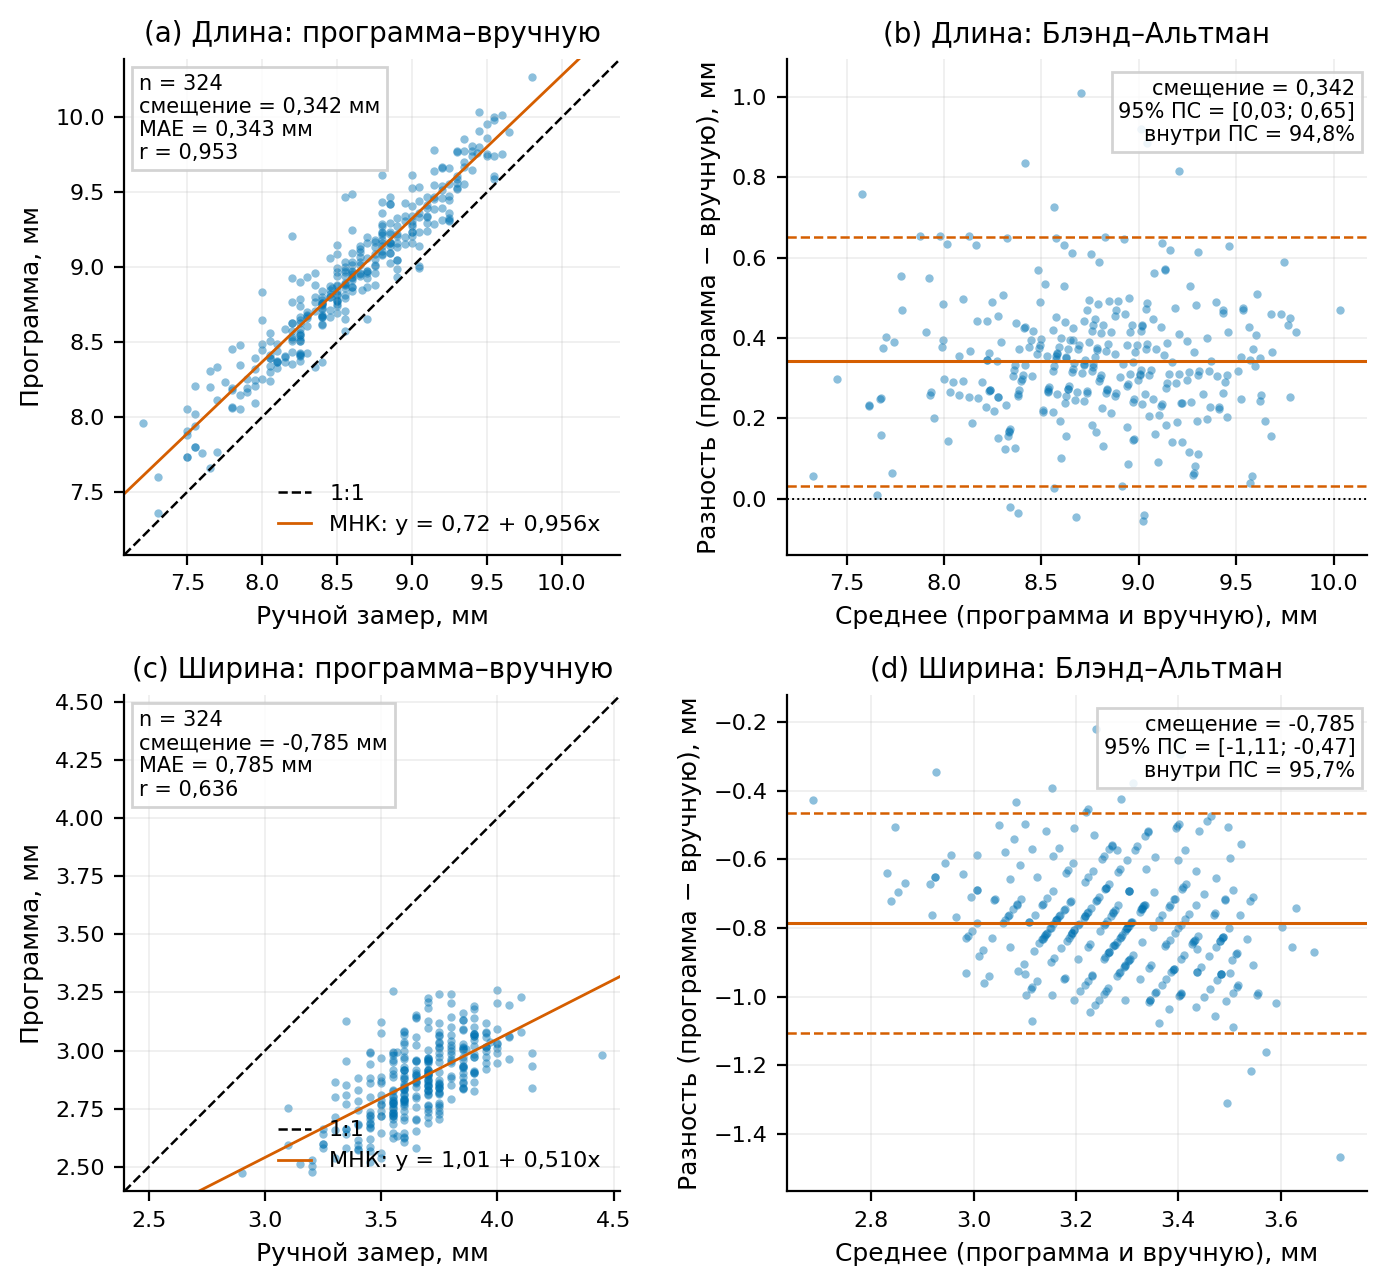
\includegraphics[width=\linewidth]{figures/fig_agreement.png}
\caption{Согласие программы с ручным измерением: (a) длина, диаграмма
рассеяния; (b) длина, Блэнд--Альтман; (c) ширина, диаграмма рассеяния;
(d) ширина, Блэнд--Альтман. Пунктир — линия равенства; оранжевая линия —
МНК; горизонтальные линии — смещение и 95\,\% пределы согласия.}
\label{fig:agreement}
\end{figure}

Регрессия $P = a + bM$ даёт $b = \LenSlope$ (95\,\% ДИ
\num{0.923}--\num{0.990}; проверка $b = 1$: $p = \num{0.010}$) и
$a = \LenIntercept$~мм (95\,\% ДИ \num{0.431}--\num{1.005}; проверка
$a = 0$: $p = 1{,}4\cdot10^{-6}$). Иными словами, программа не только
сдвинута вверх, но и немного сжимает диапазон: малым зёрнам она
добавляет больше, чем крупным. Среднее отношение \LenRatio\
(СКО \num{0.019}) также указывает на систематическое завышение, а не на
случайный шум. Робастные метрики (табл.~\ref{tab:robust}) дают ту же
картину: медиана смещения \LenMedianBias~мм, IQR \LenIqr~мм, усечённое
на 10\,\% среднее \LenTrimTen~мм, MAPE \LenMape\,\%, коэффициент
Спирмена \LenSpearman. После исключения пяти робастных выбросов
($n = \LenCleanN$) смещение \LenCleanBias~мм, MAE \LenCleanMae~мм —
вывод не меняется.

\begin{table}[htbp]
\centering\scriptsize
\setlength{\tabcolsep}{3pt}
\caption{Робастные метрики согласия (выбросы не удалены; чистые значения —
после исключения точек с $|z| > 3.5$).}
\label{tab:robust}
\begin{tabular}{@{}lrrrrrr@{}}
\toprule
Признак & \shortstack{Медиана\\смещения, мм} & IQR, мм &
\shortstack{Среднее, усечённое\\на 10\,\%, мм} & MAPE, \% &
\shortstack{$\rho$\\Спирмена} &
\shortstack{Без выбросов:\\смещение / MAE, мм} \\
\midrule
Длина & $+\num{0.332}$ & \num{0.174} & \num{0.335} & \num{4.0} & \num{-0.119} & $+\num{0.333}$ / \num{0.335} \\
Ширина & $-\num{0.791}$ & \num{0.199} & \num{-0.791} & \num{21.3} & \num{-0.583} & $-\num{0.783}$ / \num{0.783} \\
\bottomrule
\end{tabular}

\end{table}

По снимкам смещение длины меняется от $+\num{0.110}$ до
$+\num{0.627}$~мм (табл.~\ref{tab:perphoto}). Наименьшее смещение —
у non-P снимков \texttt{2\_1} и \texttt{2\_2} (\num{+0.112} и
\num{+0.110}), наибольшее — у P-снимка \texttt{2\_3p} (\num{+0.627}).
Разброс между снимками одной и той же навески — не случайный шум
калибровки: он связан с ориентацией зерна (раздел~\ref{sec:orientation}).
Это означает, что единая поправка «вычесть \num{0.342}\,мм» не будет
одинаково хороша для всех режимов съёмки.

\begin{table}[htbp]
\centering\scriptsize
\caption{Согласие по отдельным снимкам (каждый снимок сравнивается с
ручными значениями независимо; $n = 324$).}
\label{tab:perphoto}
\begin{tabular}{@{}lllrrrrrr@{}}
\toprule
Снимок & Ориентация & Фокус$^{a}$ & $\Delta L$, мм & MAE$_L$, мм & $r_L$ &
$\Delta W$, мм & MAE$_W$, мм & $r_W$ \\
\midrule
1\_1 & non-P & нет & $+\num{0.320}$ & \num{0.331} & \num{0.929} & $-\num{0.779}$ & \num{0.779} & \num{0.633} \\
1\_2 & non-P & да & $+\num{0.270}$ & \num{0.291} & \num{0.928} & $-\num{0.743}$ & \num{0.743} & \num{0.600} \\
1\_3 & non-P & нет & $+\num{0.303}$ & \num{0.315} & \num{0.934} & $-\num{0.703}$ & \num{0.703} & \num{0.519} \\
2\_1 & non-P & да & $+\num{0.112}$ & \num{0.217} & \num{0.901} & $-\num{0.895}$ & \num{0.895} & \num{0.674} \\
2\_1p & P & да & $+\num{0.496}$ & \num{0.499} & \num{0.924} & $-\num{0.777}$ & \num{0.777} & \num{0.611} \\
2\_2 & non-P & нет & $+\num{0.110}$ & \num{0.211} & \num{0.904} & $-\num{0.899}$ & \num{0.899} & \num{0.658} \\
2\_2p & P & нет & $+\num{0.497}$ & \num{0.501} & \num{0.924} & $-\num{0.768}$ & \num{0.768} & \num{0.567} \\
2\_3p & P & нет & $+\num{0.627}$ & \num{0.629} & \num{0.881} & $-\num{0.721}$ & \num{0.721} & \num{0.558} \\
\bottomrule
\end{tabular}

\end{table}

\subsection{Ширина}

По ширине картина резко иная (табл.~\ref{tab:overall},
рис.~\ref{fig:agreement}c,d). Среднее ручное значение — \num{3.665}~мм
(СКО \num{0.207}), среднее программы — \num{2.879}~мм (СКО \num{0.166}).
Смещение \WidBias~мм (95\,\% ДИ \WidBiasLo\ldots\WidBiasHi), MAE
\WidMae~мм, RMSE \WidRmse~мм, $r = \WidR$, CCC \WidCcc. Пределы
согласия — \WidLoaLo\ldots\WidLoaHi~мм; внутри лежит \num{95.68}\,\%
точек. Корреляция \num{0.636} заметно ниже, чем для длины, а CCC
практически нулевой: линейная связь есть, но согласия значений нет.
Регрессия даёт $b = \WidSlope$ (95\,\% ДИ \num{0.442}--\num{0.578}) и
$a = \WidIntercept$~мм; обе проверки ($b=1$, $a=0$) отвергаются с
$p < 10^{-13}$. Среднее отношение \WidRatio\ (СКО \num{0.038}).

На первый взгляд это выглядит как грубая ошибка ширины. Проверка
определения показывает, что это не так. Отношение \WidRatio\
статистически не отличается от $\pi/4 = \num{0.7854}$: 95\,\% ДИ
[\RatioLo; \RatioHi], $p = \RatioPi$. Предсказанное по ручному среднему
значение $\pi/4 \cdot \num{3.665} = \PiPred$~мм практически совпадает
с фактическим средним программы \PiActual~мм. Это ровно то, что должно
получиться, если ручной замер — максимальная ширина $W$, а программа —
средняя хорда $A_{\text{hull}}/L$: для эллипса $A/L = \pi W/4$. На
рис.~\ref{fig:widthdef} показана схема и реальное зерно; для него
$W_{\max} \approx \num{3.91}$~мм, $A/L \approx \num{2.83}$~мм,
отношение \num{0.724} — близко к $\pi/4$ с поправкой на неэллиптичность.

\begin{figure}[htbp]
\centering
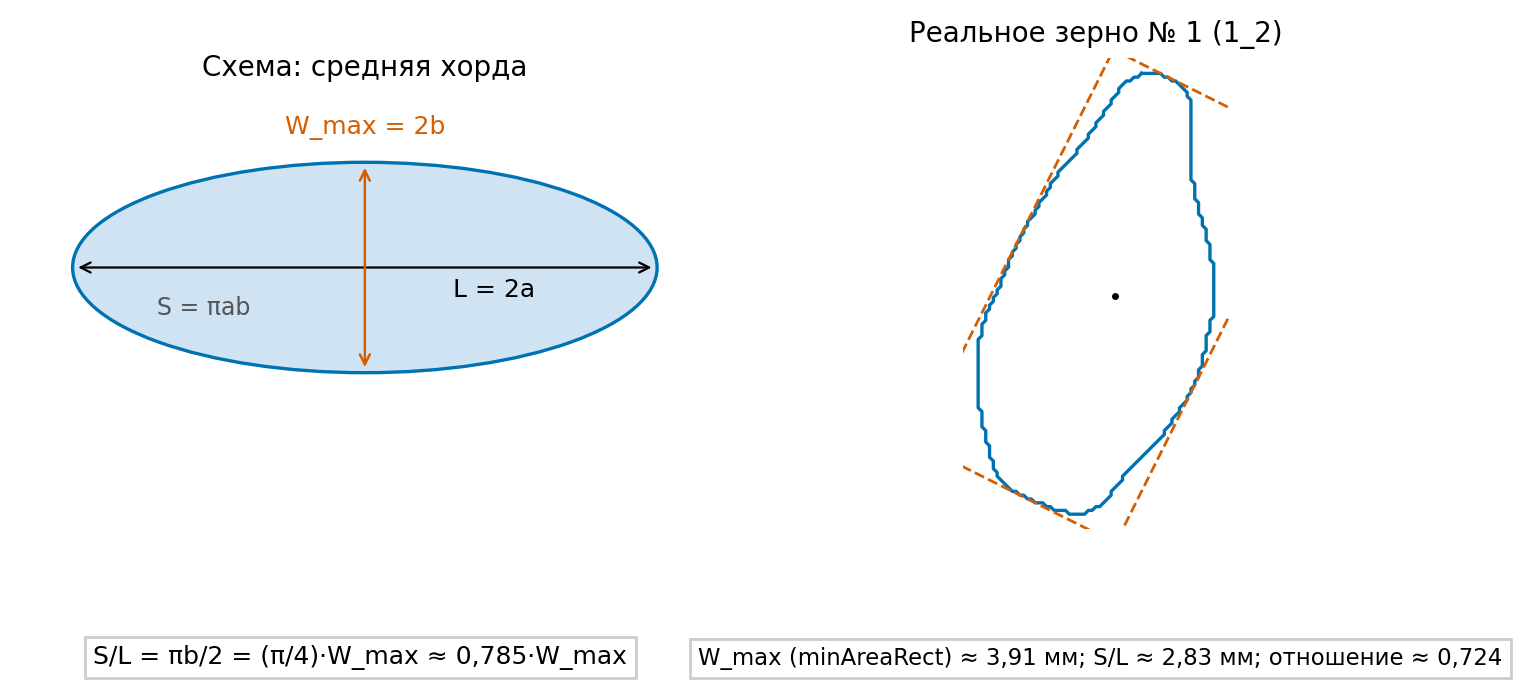
\includegraphics[width=0.95\linewidth]{figures/fig_width_definition.png}
\caption{Почему ширина программы меньше ручной: слева — эллипс, для
которого $A/L = \pi W_{\max}/4 \approx \num{0.785}\,W_{\max}$; справа —
реальное зерно с максимальной шириной по минимальному прямоугольнику и
средней хордой $A/L$.}
\label{fig:widthdef}
\end{figure}

Альтернативные геометрические определения (табл.~\ref{tab:alternatives})
подтверждают диагностику. Если вместо экспортируемой средней хорды взять
короткую сторону минимального прямоугольника, смещение становится
$+\num{0.321}$~мм, MAE \num{0.325}~мм, $r = \num{0.681}$; если взять
протяжённость поперёк оси — $+\num{0.364}$~мм и MAE \num{0.368}~мм.
Обе величины гораздо ближе к ручной максимальной ширине, чем
экспортируемая. Я не менял формулу и не выдаю эти числа за результат
программы; это диагностика того, что расхождение в первую очередь
definitional, а не следствие плохой сегментации.

\begin{table}[htbp]
\centering\scriptsize
\caption{Альтернативные определения длины и ширины (среднее по восьми
снимкам, $n = 324$). Экспортируемые величины выделены в тексте; таблица
служит только диагностикой.}
\label{tab:alternatives}
\begin{tabular}{@{}lrrrr@{}}
\toprule
Определение & Смещение [95\% ДИ], мм & MAE, мм & $r$ & Отношение \\
\midrule
экспортируемая длина (макс. хорда) & $+\num{0.342}$ [\num{0.325}; \num{0.359}] & \num{0.343} & \num{0.953} & \num{1.0401} \\
длинная сторона minAreaRect & $+\num{0.266}$ [\num{0.248}; \num{0.285}] & \num{0.274} & \num{0.948} & \num{1.0312} \\
экспортируемая ширина & $-\num{0.785}$ [\num{-0.803}; \num{-0.768}] & \num{0.785} & \num{0.636} & \num{0.7865} \\
короткая сторона minAreaRect & $+\num{0.321}$ [\num{0.301}; \num{0.340}] & \num{0.325} & \num{0.681} & \num{1.0885} \\
протяжённость поперёк оси & $+\num{0.364}$ [\num{0.345}; \num{0.384}] & \num{0.368} & \num{0.675} & \num{1.1004} \\
\bottomrule
\end{tabular}

\end{table}

Робастные метрики ширины (табл.~\ref{tab:robust}) согласуются с этим:
медиана смещения \WidMedianBias~мм, IQR \WidIqr~мм, усечённое среднее
\WidTrimTen~мм, MAPE \WidMape\,\%, коэффициент Спирмена \WidSpearman.
После исключения трёх выбросов ($n = \WidCleanN$) смещение
\WidCleanBias~мм, MAE \WidCleanMae~мм. Выбросы по ширине — это в основном
зёрна с большой ручной шириной (\num{4.45} и \num{4.15}~мм) и относительно
небольшой средней хордой; они усиливают расхождение, но не создают его.
Подробности — в приложении~В.

\subsection{Повторяемость между снимками}

Матрица «325 зёрен $\times$ 8 снимков» даёт для длины
$S_w = \LenSw$~мм, ICC(1,1) = \LenIcc\ (95\,\% ДИ \LenIccLo\ldots\LenIccHi),
RC = \LenRc~мм; для ширины $S_w = \WidSw$~мм, ICC = \WidIcc\
(95\,\% ДИ \WidIccLo\ldots\WidIccHi), RC = \WidRc~мм
(табл.~\ref{tab:repeatability}, рис.~\ref{fig:repeatability}). Для
длины это «умеренная--хорошая» повторяемость: внутризерновое СКО
составляет около \num{2.8}\,\% от среднего, ICC заметно выше нуля, но
далёк от единицы. Для ширины внутризерновое СКО мало (\num{3.4}\,\%),
однако ICC ниже, потому что межзерновая дисперсия ширины тоже невелика;
абсолютная повторяемость хорошая, а способность различать зёрна —
умеренная.

\begin{table}[htbp]
\centering\scriptsize
\setlength{\tabcolsep}{4pt}
\caption{Повторяемость по восьми снимкам: внутризерновое СКО $S_w$,
ICC(1,1) с 95\,\% ДИ и коэффициент повторяемости RC.}
\label{tab:repeatability}
\begin{tabular}{@{}lrrrrrrr@{}}
\toprule
Группа & $k$ & $S_w^{L}$, мм & ICC$_L$ [95\% ДИ] & RC$_L$, мм &
$S_w^{W}$, мм & ICC$_W$ [95\% ДИ] & RC$_W$, мм \\
\midrule
все 8 снимков & 8 & \num{0.246} & \num{0.811} [\num{0.775}; \num{0.838}] & \num{0.681} & \num{0.097} & \num{0.738} [\num{0.700}; \num{0.770}] & \num{0.267} \\
P-снимки (3) & 3 & \num{0.112} & \num{0.953} [\num{0.937}; \num{0.965}] & \num{0.311} & \num{0.045} & \num{0.939} [\num{0.924}; \num{0.954}] & \num{0.125} \\
non-P снимки (5) & 5 & \num{0.140} & \num{0.938} [\num{0.925}; \num{0.948}] & \num{0.387} & \num{0.108} & \num{0.679} [\num{0.634}; \num{0.717}] & \num{0.299} \\
заявленный лучший фокус (3) & 3 & \num{0.255} & \num{0.796} [\num{0.754}; \num{0.828}] & \num{0.707} & \num{0.105} & \num{0.678} [\num{0.626}; \num{0.721}] & \num{0.290} \\
остальные снимки (5) & 5 & \num{0.262} & \num{0.784} [\num{0.744}; \num{0.815}] & \num{0.724} & \num{0.100} & \num{0.727} [\num{0.689}; \num{0.759}] & \num{0.276} \\
\bottomrule
\end{tabular}

\end{table}

\begin{figure}[htbp]
\centering
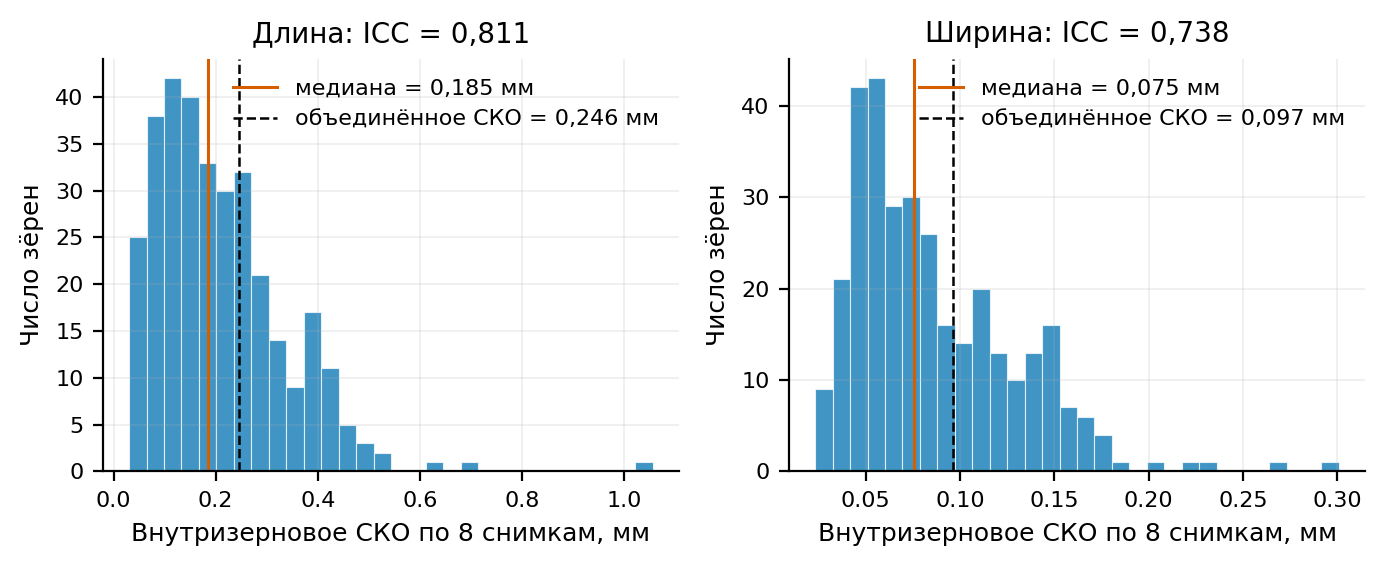
\includegraphics[width=\linewidth]{figures/fig_repeatability.png}
\caption{Распределение внутризернового СКО по восьми снимкам для длины и
ширины. Вертикальные линии — медиана и объединённое СКО.}
\label{fig:repeatability}
\end{figure}

Разбиение на подгруппы показывает, что P-снимки внутренне более
согласованы: для длины ICC \num{0.953} против \num{0.938} у non-P, для
ширины \num{0.939} против \num{0.679}. Это не означает, что P-снимки
«лучше» по смещению: как раз по длине они дают большее смещение
(раздел~\ref{sec:orientation}). Согласованность и правильность — разные
свойства, и их нельзя подменять одно другим.

Заявленные снимки «лучшего фокуса» не выделяются по повторяемости:
$S_w$ длины \num{0.255} против \num{0.262} у остальных, ICC \num{0.796}
против \num{0.784}; для ширины ICC \num{0.678} против \num{0.727}. То
есть группа «лучшего фокуса» не лучше, а по ширине даже немного хуже.
Более того, \texttt{2\_1p} — один из трёх «лучших» — имеет наибольшее
смещение длины среди P-снимков (\num{+0.496}\,мм), а \texttt{2\_3p} —
ещё больше (\num{+0.627}\,мм), хотя в «лучший фокус» не входит. Я не
могу подтвердить заявление оператора о лучшем фокусе; возможно, оно
относилось к визуальной резкости, а не к измерительной повторяемости, но
для валидации важно именно второе.

\subsection{Ориентация, статус и бороздка}
\label{sec:orientation}

Парные сравнения одного и того же зерна на P- и non-P-снимках дают
устойчивый эффект ориентации (рис.~\ref{fig:orientation}). Для пары
\texttt{2\_1p}--\texttt{2\_1} длина отличается на $+\num{0.384}$~мм
(95\,\% ДИ \num{0.352}--\num{0.416}), ширина — на $+\num{0.118}$~мм;
для пары \texttt{2\_2p}--\texttt{2\_2} — на $+\num{0.387}$ и
$+\num{0.130}$~мм соответственно. Средние P-снимков превышают средние
non-P по длине на $+\num{0.316}$~мм, по ширине — на $+\num{0.048}$~мм
(табл.~\ref{tab:paired}). Все различия имеют $p < 10^{-25}$, но
огромная значимость здесь не главное: важен размер эффекта. Смена
ориентации меняет длину почти на \num{0.4}\,мм — больше, чем среднее
смещение non-P-снимков.

\begin{figure}[htbp]
\centering
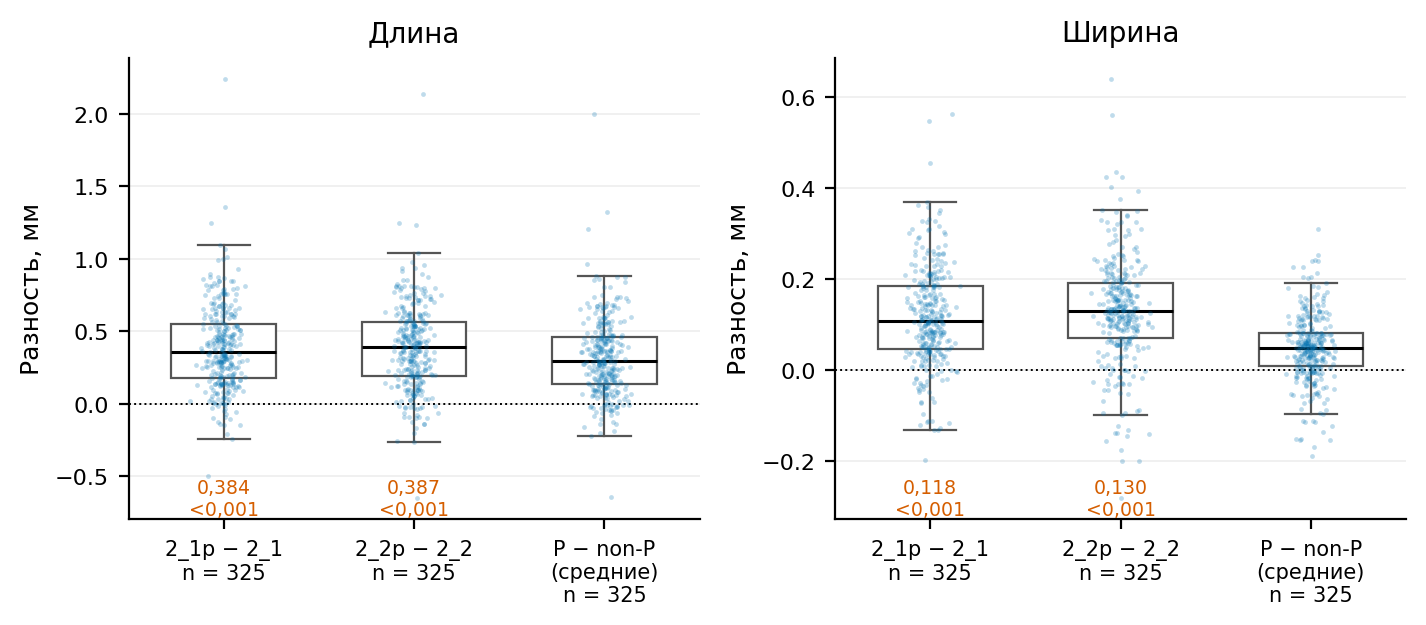
\includegraphics[width=\linewidth]{figures/fig_orientation.png}
\caption{Внутризерновые различия между P- и non-P-снимками для длины и
ширины. Точки — отдельные зёрна; на оси абсцисс — сравниваемые пары.}
\label{fig:orientation}
\end{figure}

\begin{table}[htbp]
\centering\scriptsize
\caption{Парные сравнения снимков (разность P $-$ non-P для одного и того
же зерна; $n = 325$).}
\label{tab:paired}
\begin{tabular}{@{}llrrr@{}}
\toprule
Сравнение & Параметр & $\Delta$ [95\% ДИ], мм & $p$ (парный $t$) & $r$ \\
\midrule
2\_1p $-$ 2\_1 & длина & $+\num{0.384}$ [\num{0.352}; \num{0.416}] & $5{,}4\cdot10^{-73}$ & \num{0.858} \\
2\_1p $-$ 2\_1 & ширина & $+\num{0.118}$ [\num{0.106}; \num{0.130}] & $3{,}2\cdot10^{-57}$ & \num{0.802} \\
2\_2p $-$ 2\_2 & длина & $+\num{0.387}$ [\num{0.355}; \num{0.418}] & $3{,}8\cdot10^{-74}$ & \num{0.857} \\
2\_2p $-$ 2\_2 & ширина & $+\num{0.130}$ [\num{0.117}; \num{0.143}] & $2{,}6\cdot10^{-59}$ & \num{0.783} \\
P--среднее $-$ non--P--среднее & длина & $+\num{0.316}$ [\num{0.287}; \num{0.345}] & $6{,}4\cdot10^{-64}$ & \num{0.875} \\
P--среднее $-$ non--P--среднее & ширина & $+\num{0.048}$ [\num{0.040}; \num{0.056}] & $1{,}2\cdot10^{-26}$ & \num{0.910} \\
\bottomrule
\end{tabular}

\end{table}

\begin{figure}[htbp]
\centering
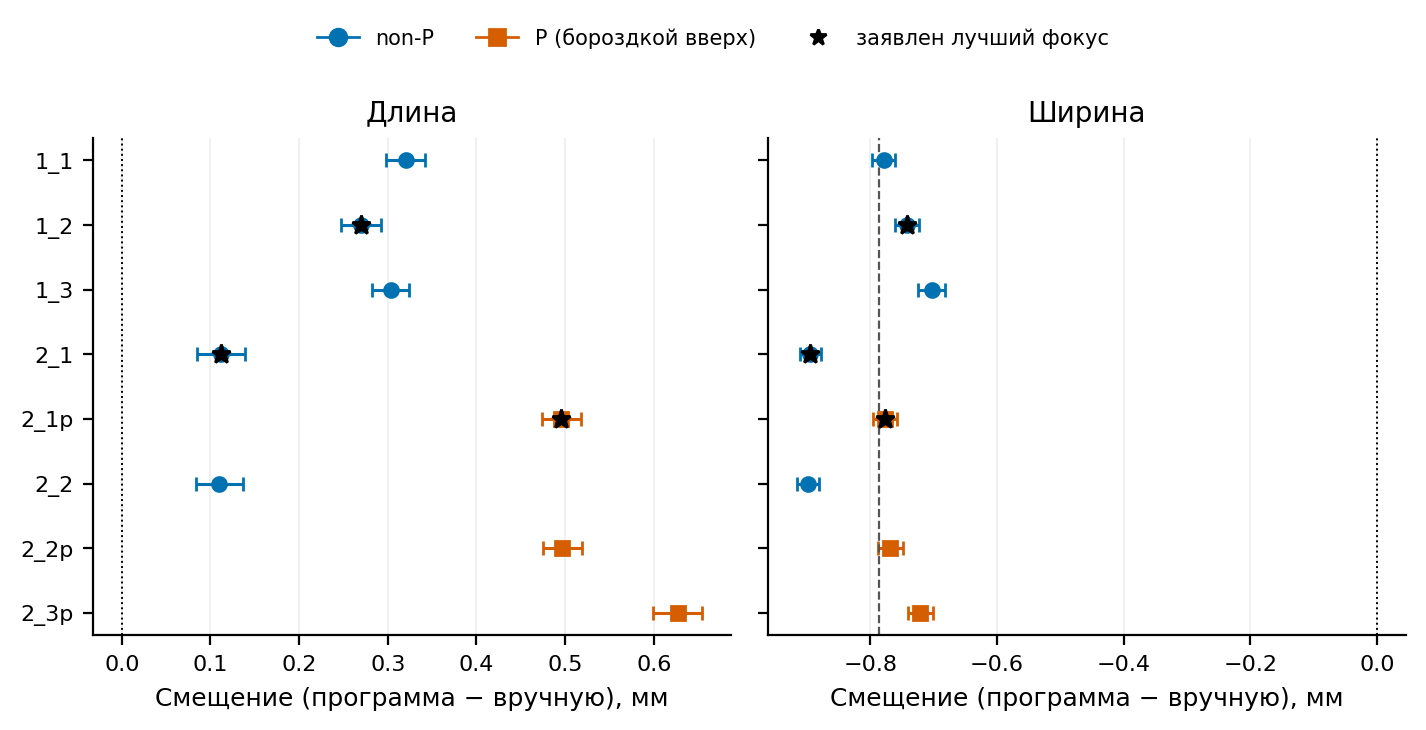
\includegraphics[width=\linewidth]{figures/fig_photo_bias.png}
\caption{Смещение программы относительно ручного замера по снимкам.
Кружки — non-P, квадраты — P, звёздочки — снимки, заявленные как «лучший
фокус». Отрезки — 95\,\% ДИ среднего смещения.}
\label{fig:photobias}
\end{figure}

Статус, который программа присваивает каждому фрагменту, связан с
внутризерновыми отклонениями, но связь неоднозначна
(табл.~\ref{tab:status}, рис.~\ref{fig:status}). Средние отклонения
длины для focused и transition близки к нулю (\num{+0.009} и
\num{-0.006}\,мм), для blurry — \num{-0.076}\,мм; СКО ширины для blurry
составляет \num{0.169}\,мм против \num{0.069} у focused. Критерий
Краскела--Уоллиса даёт $p = \num{0.0049}$ для длины и
$p = 2{,}2\cdot10^{-27}$ для ширины. Однако группы статуса не
сбалансированы (focused \num{1229} наблюдений, transition \num{1337},
blurry всего \num{34}), а статус зависит от ширины границы, то есть от
резкости и оптики; я не интерпретирую это как причинное влияние
«размытости» на измерение. Практический вывод скромнее: blurry-фрагменты
нельзя считать равноценными focused, и их доля сильно различается по
снимкам (\texttt{1\_3} — \num{18}, \texttt{1\_1} — \num{1}).

\begin{table}[htbp]
\centering\small
\caption{Внутризерновые отклонения по статусам quality control
(отклонение от среднего данного зерна по всем снимкам).}
\label{tab:status}
\begin{tabular}{@{}llrrrr@{}}
\toprule
Признак & Статус & Наблюдений & Зёрен & Среднее отклонение, мм & СКО, мм \\
\midrule
Длина & focused & 1229 & 258 & $+\num{0.009}$ & \num{0.229} \\
Длина & transition & 1337 & 314 & $-\num{0.006}$ & \num{0.231} \\
Длина & blurry & 34 & 23 & $-\num{0.076}$ & \num{0.219} \\
Ширина & focused & 1229 & 258 & $-\num{0.013}$ & \num{0.069} \\
Ширина & transition & 1337 & 314 & $+\num{0.012}$ & \num{0.103} \\
Ширина & blurry & 34 & 23 & $+\num{0.009}$ & \num{0.169} \\
\bottomrule
\end{tabular}

\end{table}

\begin{figure}[htbp]
\centering
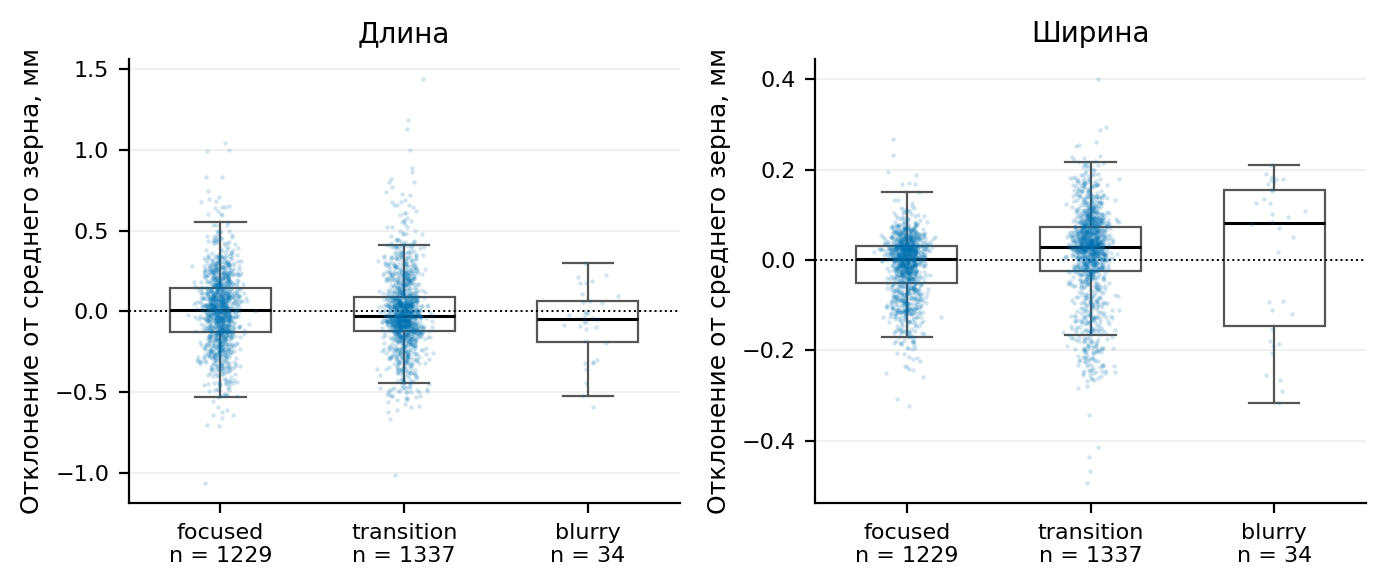
\includegraphics[width=\linewidth]{figures/fig_status.png}
\caption{Внутризерновые отклонения длины и ширины по статусам focused,
transition и blurry.}
\label{fig:status}
\end{figure}

Признак бороздки разделяет серии почти идеально: на P-снимках доля
положительных ответов \num{80.6}--\num{94.2}\,\%, на non-P —
\num{4.3}--\num{13.5}\,\% (табл.~\ref{tab:groove},
рис.~\ref{fig:groove}). Формально это отличная дискриминация ориентации.
Но порог \num{11.0} был подобран на паре \texttt{2\_1}/\texttt{2\_1p},
и эти же снимки входят в оценку; поэтому я рассматриваю результат как
описание согласованности признака с ориентацией, а не как независимую
валидацию классификатора. Снимок \texttt{2\_3p} с \num{80.6}\,\%
показывает, что запас есть не у всех P-кадров.

\begin{table}[htbp]
\centering\small
\caption{Доля зёрен с обнаруженной бороздкой по снимкам.}
\label{tab:groove}
\begin{tabular}{@{}llrrr@{}}
\toprule
Снимок & Ориентация & Положительно/всего & Доля, \% & 95\% ДИ, \% \\
\midrule
1\_1 & non-P & 31/325 & \num{9.5} & [\num{6.8}; \num{13.2}] \\
1\_2 & non-P & 44/325 & \num{13.5} & [\num{10.2}; \num{17.7}] \\
1\_3 & non-P & 22/325 & \num{6.8} & [\num{4.5}; \num{10.0}] \\
2\_1 & non-P & 14/325 & \num{4.3} & [\num{2.6}; \num{7.1}] \\
2\_1p & P & 306/325 & \num{94.2} & [\num{91.1}; \num{96.2}] \\
2\_2 & non-P & 22/325 & \num{6.8} & [\num{4.5}; \num{10.0}] \\
2\_2p & P & 297/325 & \num{91.4} & [\num{87.8}; \num{94.0}] \\
2\_3p & P & 262/325 & \num{80.6} & [\num{76.0}; \num{84.5}] \\
\bottomrule
\end{tabular}

\end{table}

\begin{figure}[htbp]
\centering
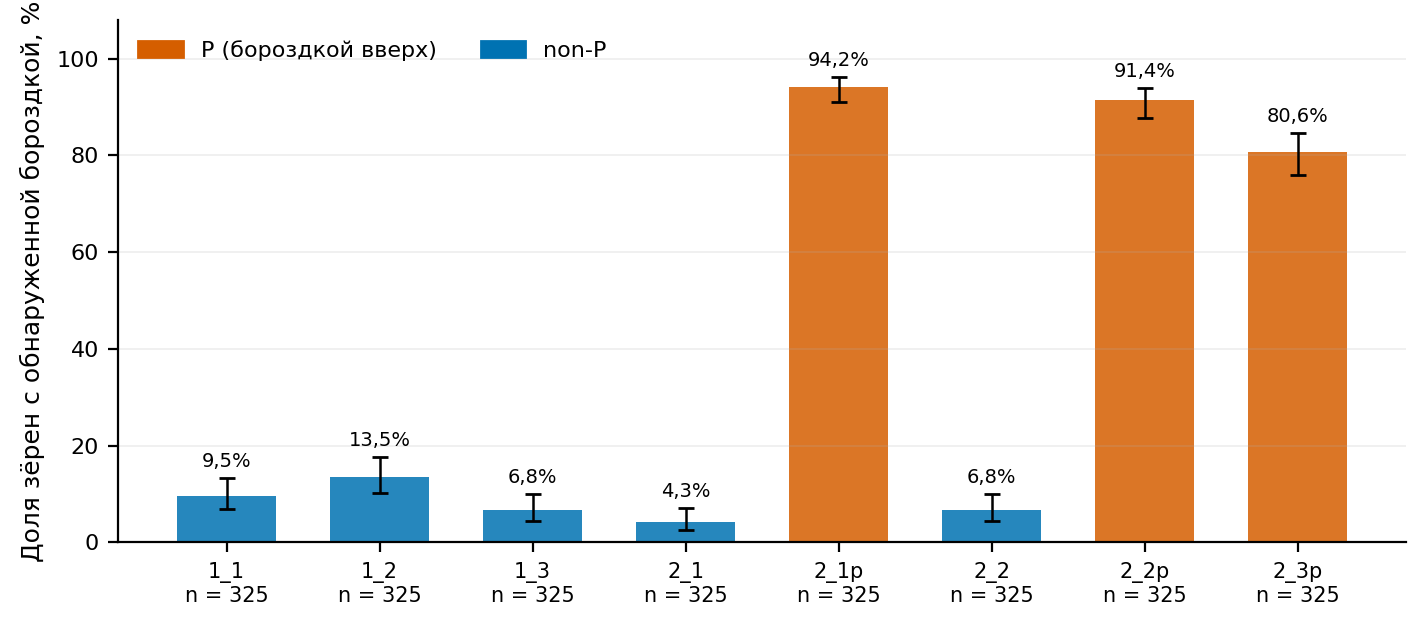
\includegraphics[width=\linewidth]{figures/fig_groove.png}
\caption{Доля зёрен с обнаруженной бороздкой; отрезки — 95\,\% ДИ.}
\label{fig:groove}
\end{figure}

\subsection{Устойчивость, выбросы и отсутствующий замер}

Робастные метрики уже приведены в табл.~\ref{tab:robust}; они не
меняют выводов. Робастный критерий $|z| > 3.5$ выделяет пять зёрен по
длине и три по ширине, без пересечения между признаками
(табл.~\ref{tab:outliers}). Все пять «длинных» выбросов — случаи
завышения программы (от \num{+0.82} до \num{+1.01}\,мм); два «ширинных»
— случаи сильного занижения (\texttt{302}: \num{4.45} против
\num{2.98}~мм; \texttt{266}: \num{4.15} против \num{2.84}~мм), один —
случай, когда программа, наоборот, завысила ширину (\texttt{221}:
\num{3.35} против \num{3.13}~мм). На рис.~\ref{fig:worst} показаны
худшие случаи; видно, что это обычные целые зёрна, а не артефакты
сегментации. Причина — форма и определение ширины, а не потеря контура.

\begin{table}[htbp]
\centering\scriptsize
\caption{Робастные выбросы ($|z| > 3.5$) по смещению; значения —
средние по восьми снимкам.}
\label{tab:outliers}
\input{tables/tex_outliers.tex}
\end{table}

\begin{figure}[htbp]
\centering
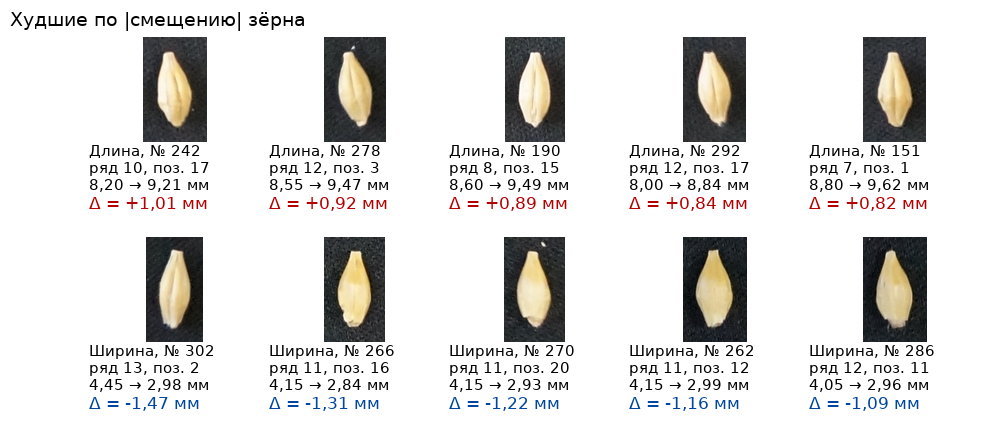
\includegraphics[width=\linewidth]{figures/fig_worst.png}
\caption{Пять худших зёрен по длине (верхний ряд) и ширине (нижний ряд).
Подписи: ручное значение $\to$ программа, ниже — смещение.}
\label{fig:worst}
\end{figure}

Отсутствие ручного замера у зерна 275 не влияет на выводы. Если
исключить весь ряд~11 (24 зерна), для оставшихся 300 зёрен смещение
длины \num{+0.339}\,мм, MAE \num{0.340}\,мм; для самого ряда~11 —
\num{+0.373} и \num{0.377}\,мм (табл.~\ref{tab:subgroups}). Разница
составляет сотые доли миллиметра. Более того, тест по изображениям
показывает, что положение пропуска в ряду не определяется однозначно:
лучшая MAE достигается при $k = 19$, а не при $k = 25$
(рис.~\ref{fig:missingk}). Я всё равно использую $k = 25$, потому что
это следует из физической структуры укладки (25 лунок в ряду) и
подтверждается прямым мапированием рядов 12--13; но признаю, что
изображения сами по себе не дают однозначного ответа. На выводы это не
влияет: чувствительность к ряду~11 мала.

\begin{table}[htbp]
\centering\scriptsize
\caption{Чувствительность к ряду~11 и подгруппам снимков.}
\label{tab:subgroups}
\begin{tabular}{@{}lrrrrrrr@{}}
\toprule
Подгруппа & $n$ & $\Delta L$, мм & MAE$_L$, мм & $r_L$ &
$\Delta W$, мм & MAE$_W$, мм & $r_W$ \\
\midrule
Все зёрна & 324 & $+\num{0.342}$ & \num{0.343} & \num{0.953} & $-\num{0.785}$ & \num{0.785} & \num{0.636} \\
Без ряда 11 & 300 & $+\num{0.339}$ & \num{0.340} & \num{0.953} & $-\num{0.785}$ & \num{0.785} & \num{0.648} \\
Только ряд 11 & 24 & $+\num{0.373}$ & \num{0.377} & \num{0.954} & $-\num{0.793}$ & \num{0.793} & \num{0.534} \\
P-снимки & 324 & $+\num{0.540}$ & \num{0.543} & \num{0.918} & $-\num{0.755}$ & \num{0.755} & \num{0.584} \\
non-P снимки & 324 & $+\num{0.223}$ & \num{0.251} & \num{0.929} & $-\num{0.804}$ & \num{0.804} & \num{0.646} \\
Заявленный лучший фокус & 324 & $+\num{0.293}$ & \num{0.297} & \num{0.947} & $-\num{0.805}$ & \num{0.805} & \num{0.662} \\
Остальные снимки & 324 & $+\num{0.371}$ & \num{0.372} & \num{0.954} & $-\num{0.774}$ & \num{0.774} & \num{0.616} \\
\bottomrule
\end{tabular}

\end{table}

\begin{figure}[htbp]
\centering
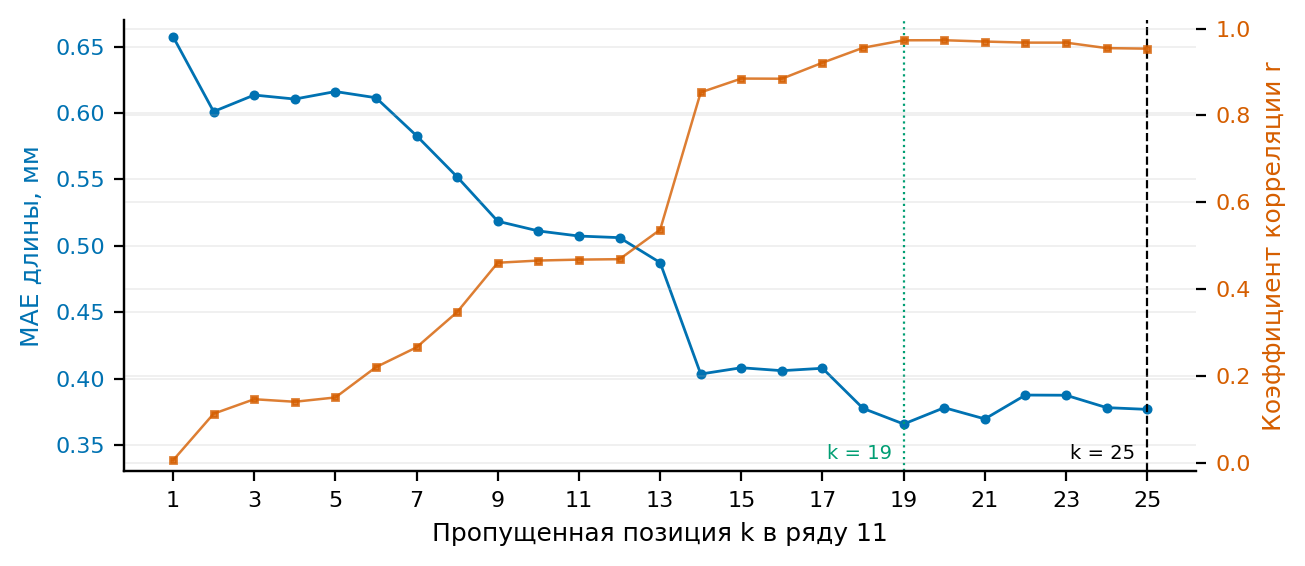
\includegraphics[width=0.9\linewidth]{figures/fig_missing_k.png}
\caption{Тест положения пропуска в ряду~11: MAE длины и корреляция в
зависимости от предполагаемого $k$. Минимум MAE — при $k = 19$;
структурное значение $k = 25$ отмечено пунктиром.}
\label{fig:missingk}
\end{figure}

Пространственное распределение смещений по рядам и позициям
(рис.~\ref{fig:grid}) не показывает крупных локальных аномалий:
смещение длины по рядам меняется от \num{+0.286} до \num{+0.419}\,мм,
ширины — от \num{-0.746} до \num{-0.812}\,мм (табл.~\ref{tab:byrow}).
Это ещё один аргумент против гипотезы «одно плохое зерно или один
сбойный участок кадра испортил статистику». Разброс между снимками
(рис.~\ref{fig:photobias}) при этом остаётся главным источником
неоднородности.

\begin{figure}[htbp]
\centering
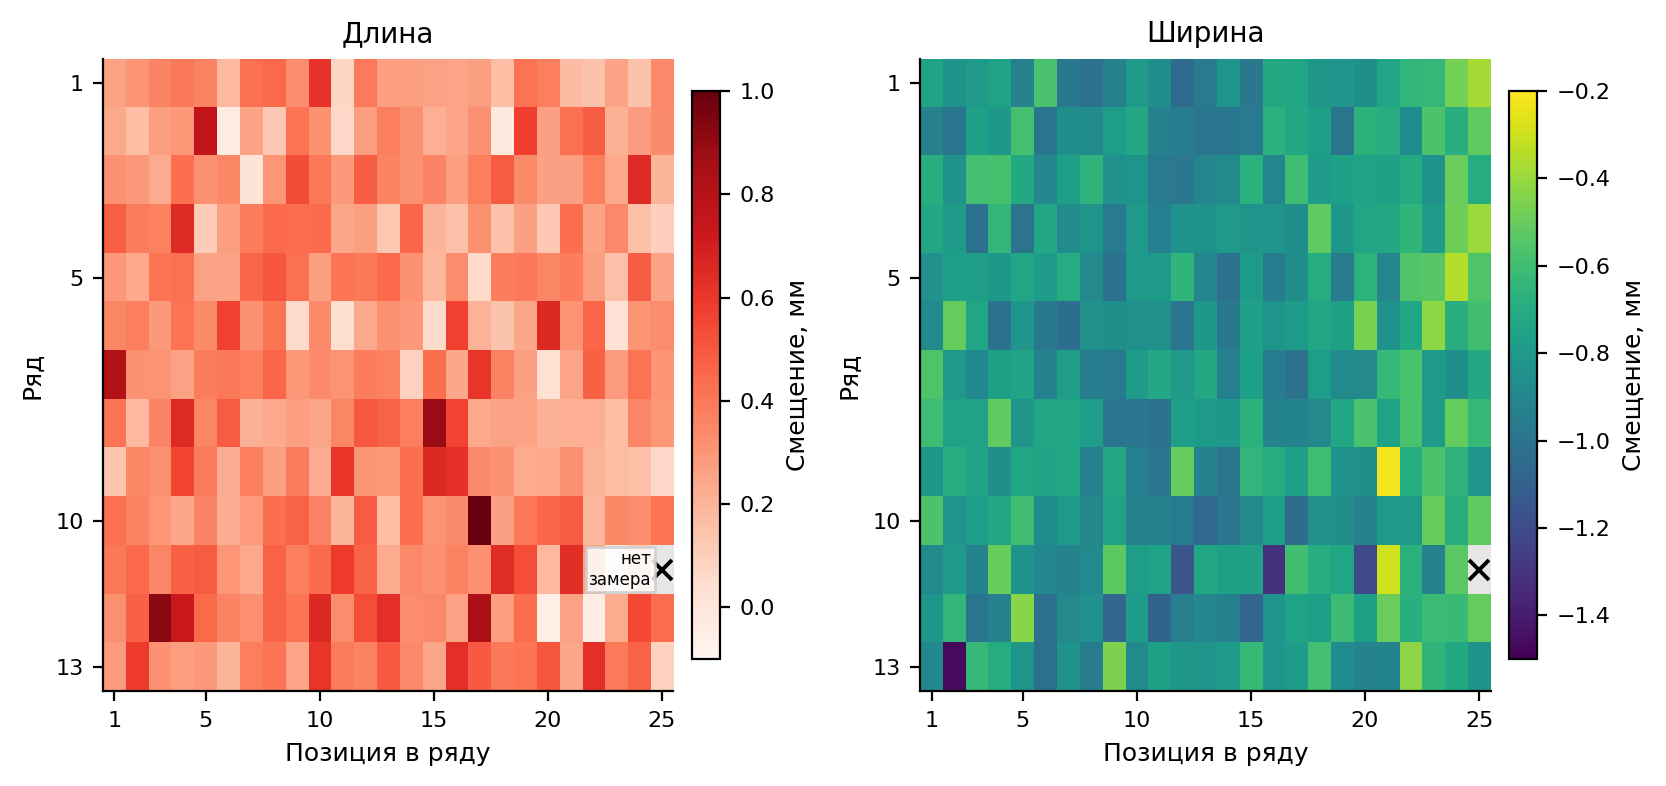
\includegraphics[width=\linewidth]{figures/fig_grid.png}
\caption{Тепловые карты смещений по рядам и позициям укладки (среднее по
восьми снимкам). Крестик — отсутствующий ручной замер.}
\label{fig:grid}
\end{figure}

\subsection{Дополнительные проверки}

Факторы снимка — масштаб, медианная яркость, разброс яркости, медианная
ширина границы — не показали убедительной связи со смещением
(табл.~\ref{tab:factors}). При $n = 8$ корреляции слабые и
незначимые: например, для длины с \texttt{mm\_per\_px} $r = \num{0.395}$
($p = \num{0.333}$), с яркостью $r = \num{-0.185}$ ($p = \num{0.661}$);
для ширины с шириной границы $r = \num{0.558}$ ($p = \num{0.150}$).
Я не делаю из этого вывода «факторов нет»: мощность мала, а масштаб и
яркость к тому же связаны с настройками съёмки. Можно лишь сказать, что
в этих восьми кадрах нет сильного кандидата на объяснение смещения,
кроме ориентации.

\begin{table}[htbp]
\centering\scriptsize
\setlength{\tabcolsep}{3pt}
\caption{Факторы снимков и смещения (средние по снимку).}
\label{tab:factors}
\begin{tabular}{@{}lrrrrrr@{}}
\toprule
Снимок & \shortstack{Масштаб,\\мм/px} & \shortstack{Медианная\\яркость} &
\shortstack{Разброс яркости\\(СКО)} &
\shortstack{Медиана ширины\\границы, px} & $\Delta L$, мм & $\Delta W$, мм \\
\midrule
1\_1 & \num{0.068465} & \num{205.0} & \num{9.1} & \num{3.92} & $+\num{0.320}$ & $-\num{0.779}$ \\
1\_2 & \num{0.066822} & \num{203.0} & \num{7.5} & \num{4.08} & $+\num{0.270}$ & $-\num{0.743}$ \\
1\_3 & \num{0.063253} & \num{200.0} & \num{8.0} & \num{4.85} & $+\num{0.303}$ & $-\num{0.703}$ \\
2\_1 & \num{0.066270} & \num{209.7} & \num{8.7} & \num{3.47} & $+\num{0.112}$ & $-\num{0.895}$ \\
2\_1p & \num{0.064464} & \num{194.3} & \num{9.6} & \num{3.71} & $+\num{0.496}$ & $-\num{0.777}$ \\
2\_2 & \num{0.063195} & \num{191.3} & \num{8.7} & \num{3.99} & $+\num{0.110}$ & $-\num{0.899}$ \\
2\_2p & \num{0.063944} & \num{193.7} & \num{8.9} & \num{3.82} & $+\num{0.497}$ & $-\num{0.768}$ \\
2\_3p & \num{0.070832} & \num{203.0} & \num{8.7} & \num{3.84} & $+\num{0.627}$ & $-\num{0.721}$ \\
\bottomrule
\end{tabular}

\end{table}

Цветовая стабильность высокая: медианное внутризерновое СКО яркости
составляет \num{7.57} (в единицах 0--255), а корреляции «СКО яркости —
СКО длины» и «СКО яркости — СКО ширины» близки к нулю
($\rho = \num{-0.058}$, $p = \num{0.294}$ и $\rho = \num{-0.047}$,
$p = \num{0.395}$). Это не центральный результат, но он показывает, что
фотометрическая нестабильность между кадрами не объясняет
геометрическую вариацию.

\section{Обсуждение}

\subsection{Что показала валидация}

Главный результат работы — асимметрия между длиной и шириной. По длине
программа даёт значения, которые тесно связаны с ручными
($r = \num{0.953}$), имеют умеренное систематическое смещение
($+\num{0.342}$~мм, около \num{4}\,\%) и приемлемую для многих
прикладных задач повторяемость (ICC \num{0.811}). По ширине связь
слабее ($r = \num{0.636}$), а согласие практически отсутствует
(CCC \num{0.063}) из-за смещения $-\num{0.785}$~мм. Это не означает,
что программа «плохо сегментирует»: контуры находятся устойчиво, а
расхождение по ширине объясняется определением измеряемой величины.
Именно поэтому валидация должна была включать не только корреляцию, но
и проверку того, что именно экспортируется.

Для длины наиболее вероятны несколько совместных причин. Программная
длина — это наибольшая внутренняя хорда между крайними точками контура,
тогда как штангенциркуль измеряет расстояние между губками, которые
касаются зерна в двух точках и не обязательно захватывают тонкий кончик
или ость. Контур, построенный по порогу яркости, может включать тень или
светлый ореол у края, что добавляет несколько пикселей с каждой стороны;
при масштабе около \num{0.065}\,мм/px это даёт сотые доли миллиметра, но
не все \num{0.34}\,мм. Наконец, наклонная укладка и ориентация меняют,
какая проекция зерна видна камере. Один механизм не объясняет весь
эффект; скорее, это сумма геометрического определения, краевой
сегментации и ориентации. Регрессия с $b = \num{0.956}$ и
$a = \num{0.718}$ показывает, что смещение не сводится к постоянному
сдвигу: у мелких зёрен относительная ошибка больше. Поэтому простая
поправка «вычесть \num{0.342}\,мм» уменьшит среднее смещение, но не
сделает значения полностью эквивалентными ручным.

Для ширины картина гораздо чище. Среднее отношение \WidRatio\
практически совпадает с $\pi/4$, а предсказание по ручному среднему
отличается от фактического на \num{0.001}\,мм. Это сильный
количественный аргумент в пользу того, что программа измеряет среднюю
хорду, а ручной эталон — максимальную ширину. Для эллипса эти величины
связаны именно множителем $\pi/4$; для реального зерна с бороздкой и
неэллиптическим контуром отношение немного варьирует, что и даёт
разброс \num{0.038}. Следовательно, ширина программы не является
«ошибочной» в смысле алгоритма: она просто отвечает на другой вопрос.
Если пользователь хочет получить максимальную ширину, текущую формулу
надо менять; если нужна средняя ширина или характеристика площади,
формула осмысленна, но её нельзя сравнивать со штангенциркулем без
пересчёта. Альтернативная короткая сторона минимального прямоугольника
даёт гораздо лучшее согласие (смещение $+\num{0.321}$~мм, MAE
\num{0.325}~мм), но и она не идеальна: ручная максимальная ширина и
максимальная ширина прямоугольника — не одно и то же, особенно для
зёрен с неровным краем.

\subsection{Повторяемость, ориентация и фокус}

Повторяемость длины (ICC \num{0.811}) и ширины (ICC \num{0.738}) я
считаю умеренной. Внутризерновое СКО длины \num{0.246}\,мм — это около
\num{2.8}\,\% среднего; для сравнения, среднее смещение длины
\num{0.342}\,мм. То есть вариация между снимками не исчезает на фоне
систематического смещения и должна учитываться, если программа
используется для отбора. Ширина внутри снимков стабильнее
($S_w = \num{0.097}$~мм), но её межзерновая вариация мала, поэтому ICC
ниже; это не противоречие, а разные аспекты надёжности.

Ориентация — самый сильный фактор, который я обнаружил. Парные сравнения
одного и того же зерна показывают, что P-снимки («бороздкой вверх») дают
длину в среднем на \num{0.316}\,мм больше, чем non-P, и ширину на
\num{0.048}\,мм больше. Для длины это почти равно среднему смещению
non-P-снимков ($+\num{0.223}$~мм) и больше, чем разница между
«лучшим фокусом» и остальными. Практический вывод: нельзя смешивать
снимки разных ориентаций в одной калибровке без проверки. P-снимки
внутренне более согласованы (ICC длины \num{0.953}, ширины
\num{0.939}), но по длине сильнее смещены; non-P ближе к ручному
эталону по длине, но менее стабильны. Выбор режима зависит от цели: для
ранжирования внутри одной серии лучше P, для сопоставления с ручными
абсолютными значениями — non-P, но и там смещение остаётся.

Заявление оператора о трёх «лучших» снимках не подтвердилось по
повторяемости: группа «лучшего фокуса» имела $S_w$ длины \num{0.255}
против \num{0.262} и ICC \num{0.796} против \num{0.784}, а по ширине
была хуже (\num{0.678} против \num{0.727}). Один из «лучших» снимков,
\texttt{2\_1p}, дал одно из наибольших смещений длины. Возможны
объяснения: визуальная резкость оценивалась по всему кадру, а не по
краям зёрен; фокус мог быть неравномерным по полю; наконец, «лучший
фокус» мог означать отсутствие смаза, а не оптимальную резкость
контура. Для валидации важен измерительный результат, а не визуальное
впечатление. Статус blurry тоже неоднозначен: средние отклонения малы,
но разброс ширины больше, а группа малочисленна (\num{34} наблюдения,
\num{23} зерна), поэтому я не исключал blurry-фрагменты и не делал
выводов о причинности.

\subsection{Калибровка и технические риски}

Автоматическая калибровка работала на этих восьми снимках: расхождение
с независимой оценкой по штрихам линейки не превысило \num{2.1}\,\%,
среднее смещение статистически неотличимо от нуля. Этого достаточно,
чтобы исключить калибровку как главную причину смещения длины или
ширины. Но реализация опирается на безусловное умножение на 2, то есть
на предположение, что детектор видит половинные штрихи. Если на другом
снимке детектор увидит полные миллиметровые штрихи, результат
удвоится; если линейка будет другой или кадр обрезан иначе, поведение
непредсказуемо. Я считаю это главным техническим риском программы,
который не проявляется на данной серии, но может проявиться при
расширении использования. Правильное исправление — не «магическая»
двойка, а устойчивое определение типа штриха (сантиметровые,
полумиллиметровые, миллиметровые) и проверка на эталонном объекте; но это
выходит за рамки валидации «как есть».

\subsection{Ручной эталон и влажность}

Ручной файл — не идеальный эталон. В нём нет протокола: неясно, какая
именно ширина измерялась (максимальная, в средней части, по бороздке),
сколько раз, одним ли оператором, как фиксировалось зерно. Значения
лежат на сетке \num{0.05}\,мм, а не \num{0.1}\,мм, как заявил оператор;
это меняет интерпретацию точности, хотя на фоне смещения
\num{0.34}--\num{0.79}\,мм квантование мало. Повторных ручных замеров
нет, поэтому межоператорская и внутриоператорская ошибка не оценены;
наблюдаемое смещение включает и ошибку эталона. Для ширины это менее
критично, потому что отношение $\pi/4$ объясняет расхождение
систематически, а не случайно. Для длины нельзя исключить, что часть
\num{0.34}\,мм — это разница между «хордой по контуру» и «губками
штангенциркуля».

Влажность зерна не измерялась. Размеры зерна меняются при увлажнении и
высыхании, а штангенциркуль и оптический метод по-разному реагируют на
деформацию и нажим губок. Поскольку обе величины получены в одной
серии и, вероятно, в близких условиях, это не объясняет разницу между
длиной и шириной, но ограничивает перенос абсолютных значений на
другую влажность. Для строгой метрологии нужны контроль влажности,
термостабилизация и повторные замеры эталона; в данной работе это
открытый вопрос, а не измеренный фактор.

\subsection{Внешняя валидность и литература}

Работа ограничена одной навеской, одной укладкой, одной серией
освещения и восемью кадрами. Все зёрна целые, не соприкасаются, лежат
примерно в одной плоскости; программа не проверялась на слипшихся,
повреждённых, проросших или сильно изогнутых зёрнах, на других сортах и
на других разрешениях. Поэтому вывод «длина пригодна для ранжирования,
ширина требует переопределения» относится к целым зёрнам данной
навески; перенос на производственную практику требует отдельной
валидации. Это не формальность: ориентационный эффект
\num{0.316}\,мм показывает, что даже смена укладки может сместить
результат сильнее, чем различия между близкими сортами.

Литература по фенотипированию семян подтверждает, что изображения дают
устойчивые размеры и форму, но подчёркивает зависимость результатов от
определений и протокола \cite{li2014,tanabata2012,igathinathane2008}.
SmartGrain и аналогичные инструменты обычно сообщают высокие
корреляции с эталоном для длины и площади; мои \num{0.953} для длины
согласуются с этим уровнем. Для ширины сравнение сложнее: разные
работы используют максимальную ширину, ширину по Фере, среднюю хорду
или короткую сторону прямоугольника, и эти величины не
взаимозаменяемы. Мой результат — количественная иллюстрация того, что
без явного определения ширины высокая корреляция может сочетаться с
нулевым согласием. Это, на мой взгляд, более полезный вывод, чем ещё
одно подтверждение «изображения работают».

\subsection{Практические следствия}

Если программа используется как есть, я бы рекомендовал: (1) не
сравнивать экспортируемую ширину со штангенциркулем и явно называть её
средней хордой; (2) для длины либо вводить калибровку на независимой
выборке, либо использовать только ранжирование и относительные
различия; (3) не смешивать P- и non-P-снимки в одной серии без
поправочных коэффициентов; (4) фиксировать ориентацию и протокол
укладки; (5) заменить безусловное умножение на 2 в калибровке на
проверяемое правило; (6) сохранять журнал прогонов и контрольные
объекты. Ни один из этих пунктов не является «настройкой под эталон»:
это либо документирование определения, либо устранение технического
риска.

\section{Заключение}

Я провёл валидацию разработанной программы на восьми фотографиях одной
навески ячменя (325 зёрен) и сопоставил её с 324 ручными замерами.
Сегментация и сопоставление данных оказались устойчивыми: все 325 зёрен
найдены на всех снимках, структура 13$\times$25 восстановлена,
повторный прогон детерминирован, калибровка согласуется с независимой
оценкой в пределах около \num{2}\,\%.

По длине программа систематически завышает значение на
\num{0.342}\,мм (около \num{4}\,\%), имеет MAE \num{0.343}\,мм,
$r = \num{0.953}$ и CCC \num{0.781}. Это позволяет использовать длину
для ранжирования и относительных сравнений, но не делает её
взаимозаменяемой с ручным измерением в абсолютной шкале. По ширине
смещение составляет \num{-0.785}\,мм, MAE \num{0.785}\,мм,
$r = \num{0.636}$, CCC \num{0.063}; отношение \WidRatio\
статистически совпадает с $\pi/4$, что указывает на определение ширины
как средней хорды, а не на ошибку сегментации. В текущем виде ширина
программы не сопоставима с максимальной шириной по штангенциркулю.

Повторяемость между снимками умеренная: ICC(1,1) \num{0.811} для длины
и \num{0.738} для ширины. Ориентация зерна меняет длину примерно на
\num{0.316}\,мм, поэтому протокол съёмки должен быть единым.
Заявление о трёх «лучших по фокусу» снимках не подтверждается
повторяемостью; статус blurry связан с большим разбросом ширины, но
причинность не установлена. Калибровочный коэффициент~2 работает на
данной серии, но остаётся хрупким и недокументированным риском.

\section{Краткое резюме}

\paragraph{Что получилось.}
Пакетная обработка устойчива: 325/325 зёрен на всех восьми снимках, ноль
ошибок сопоставления, детерминированный повторный прогон. Масштаб
согласуется с независимой оценкой в пределах \num{2.1}\,\%. Длина
показывает высокую корреляцию с ручным эталоном ($r = \num{0.953}$),
умеренное смещение \num{0.342}\,мм и повторяемость ICC \num{0.811};
для ранжирования она пригодна, а абсолютные значения требуют
калибровки на независимой выборке.
Повторяемость ширины хорошая ($S_w = \num{0.097}$~мм, ICC \num{0.738}),
а её расхождение с ручным эталоном объясняется определением средней
хорды.

\paragraph{Что не получилось.}
Абсолютные значения длины не эквивалентны ручным: смещение
\num{0.342}\,мм, пределы согласия \num{0.03}--\num{0.65}\,мм, наклон
регрессии \num{0.956}. Ширина в текущем виде не является максимальной
шириной: смещение \num{-0.785}\,мм, CCC \num{0.063}, отношение
\WidRatio\ вместо ожидаемого пользователем \num{1.0}. Заявленный
«лучший фокус» не подтверждён. Калибровочное умножение на 2 не
обосновано в коде и может сломаться на других данных. Ручной протокол
не документирован, поэтому часть смещения длины может относиться к
эталону.

\paragraph{Допущения.}
Принято, что серийный номер ручного файла напрямую соответствует номеру
программы (проверено структурой рядов и тестом сдвига); что ручная
ширина — максимальная ширина, а ручная длина — максимальная длина; что
все восемь снимков изображают одни и те же физические зёрна; что
пиксели квадратные, масштаб равномерный, а перспективные искажения
пренебрежимо малы; что влажность и условия съёмки не менялись
существенно; что отсутствие замера у зерна 275 не смещает нумерацию.
Утверждения оператора о навеске, ориентации и фокусе рассматриваются
как заявления, а не как независимо проверенные факты.

\paragraph{Открытые вопросы.}
Неясно, какую именно ширину измерял оператор и с какой повторяемостью;
не проверено, как на длину влияют ости, кончики и краевой ореол; не
оценена межоператорская ошибка ручных замеров; не измерена влажность;
не проверены другие сорта, навески, разрешения и условия освещения; не
проверена устойчивость калибровочного коэффициента~2 на других
линейках; не валидированы толщина и масса, которых нет в пакетном
экспорте. Для ответа на эти вопросы нужны повторные ручные замеры,
эталонные объекты, контроль влажности и независимая выборка.

\begin{thebibliography}{99}

\bibitem{bland1986}
Bland J.M., Altman D.G. Statistical methods for assessing agreement between
two methods of clinical measurement // The Lancet. 1986. Vol.~327, no.~8476.
P.~307--310. DOI: 10.1016/S0140-6736(86)90837-8.

\bibitem{lin1989}
Lin L.I.-K. A concordance correlation coefficient to evaluate
reproducibility // Biometrics. 1989. Vol.~45, no.~1. P.~255--268.
DOI: 10.2307/2532051.

\bibitem{shrout1979}
Shrout P.E., Fleiss J.L. Intraclass correlations: uses in assessing rater
reliability // Psychological Bulletin. 1979. Vol.~86, no.~2.
P.~420--428. DOI: 10.1037/0033-2909.86.2.420.

\bibitem{kruskal1952}
Kruskal W.H., Wallis W.A. Use of ranks in one-criterion variance analysis //
Journal of the American Statistical Association. 1952. Vol.~47, no.~260.
P.~583--621. DOI: 10.1080/01621459.1952.10483441.

\bibitem{vanderwalt2014}
van der Walt S., Sch\"onberger J.L., Nunez-Iglesias J., Boulogne F.,
Warner J.D., Yager N., Gouillart E., Yu T. scikit-image: image processing
in Python // PeerJ. 2014. Vol.~2. Art.~e453. DOI: 10.7717/peerj.453.

\bibitem{virtanen2020}
Virtanen P., Gommers R., Oliphant T.E., Haberland M., Reddy T.,
Cournapeau D., et al. SciPy 1.0: fundamental algorithms for scientific
computing in Python // Nature Methods. 2020. Vol.~17, no.~3.
P.~261--272. DOI: 10.1038/s41592-019-0686-2.

\bibitem{harris2020}
Harris C.R., Millman K.J., van der Walt S.J., Gommers R., Virtanen P.,
Cournapeau D., et al. Array programming with NumPy // Nature. 2020.
Vol.~585, no.~7825. P.~357--362. DOI: 10.1038/s41586-020-2649-2.

\bibitem{bradski2000}
Bradski G. The OpenCV Library // Dr. Dobb's Journal of Software Tools.
2000. Vol.~25, no.~11. P.~120--125.

\bibitem{li2014}
Li L., Zhang Q., Huang D. A review of imaging techniques for plant
phenotyping // Sensors. 2014. Vol.~14, no.~11. P.~20078--20111.
DOI: 10.3390/s141120078.

\bibitem{tanabata2012}
Tanabata T., Shibaya T., Hori K., Ebana K., Yano M. SmartGrain:
high-throughput phenotyping software for measuring seed shape through image
analysis // Plant Physiology. 2012. Vol.~160, no.~4. P.~1871--1880.
DOI: 10.1104/pp.112.205120.

\bibitem{igathinathane2008}
Igathinathane C., Pordesimo L.O., Columbus E.P., Batchelor W.D.,
Methuku S.R. Shape identification and particles size distribution from
basic shape parameters using ImageJ // Computers and Electronics in
Agriculture. 2008. Vol.~63, no.~2. P.~168--182.
DOI: 10.1016/j.compag.2008.02.007.

\bibitem{symons1988}
Symons S.J., Fulcher R.G. Determination of wheat kernel morphological
variation by digital image analysis: I. Variation in Eastern Canadian
milling quality wheats // Journal of Cereal Science. 1988. Vol.~8, no.~3.
P.~211--218. DOI: 10.1016/S0733-5210(88)80032-8.

\bibitem{sankaran2016}
Sankaran S., Wang M.H., Vandemark G.J. Image-based rapid phenotyping of
chickpeas seed size // Engineering in Agriculture, Environment and Food.
2016. Vol.~9, no.~1. P.~50--55. DOI: 10.1016/j.eaef.2015.06.001.

\bibitem{gao2017}
Gao J., White S.A., Palaniappan K., Warmund M.R., Bunyak F. Museed: a
mobile image analysis application for plant seed morphometry // 2017 IEEE
International Conference on Image Processing (ICIP). 2017. P.~2826--2830.
DOI: 10.1109/ICIP.2017.8296798.

\end{thebibliography}

\appendix

\begin{landscape}
\section{Полная таблица сопоставления по зёрнам}

В табл.~\ref{tab:full} приведены все 325 зёрен. Для каждого зерна указаны
ручные длина $L$, ширина $W$, толщина $T$ и масса $m$; программные
$L_{\text{прог}}$ и $W_{\text{прог}}$ — среднее по восьми снимкам, в
скобках — внутризерновое СКО. Разности $\Delta L$ и $\Delta W$ равны
«программа минус ручной замер». Прочерк в строке 275 означает
отсутствие ручного замера; программные значения для этого зерна есть.
Толщина и масса приведены только для справки: программа их не
экспортирует, и они не валидируются. В последнем столбце метки
\texttt{L} и \texttt{W} отмечают робастные выбросы по длине и ширине
соответственно.

\begingroup
\scriptsize
\setlength{\tabcolsep}{3pt}
\setlength{\LTcapwidth}{\linewidth}
\begin{longtable}{@{}rrrrrrrrrrrr@{}}
\caption{Полная таблица сопоставления по зёрнам (325 строк; программа — среднее
и внутризерновое СКО по 8 снимкам).}\label{tab:full}\\
\toprule
№ & Ряд & Поз. & $L_{\text{руч}}$ & $W_{\text{руч}}$ & $T_{\text{руч}}$ &
$m_{\text{руч}}$, г & $L_{\text{прог}}$ (СКО) & $W_{\text{прог}}$ (СКО) &
$\Delta L$ & $\Delta W$ & Примечание \\
\midrule
\endfirsthead
\toprule
№ & Ряд & Поз. & $L_{\text{руч}}$ & $W_{\text{руч}}$ & $T_{\text{руч}}$ &
$m_{\text{руч}}$, г & $L_{\text{прог}}$ (СКО) & $W_{\text{прог}}$ (СКО) &
$\Delta L$ & $\Delta W$ & Примечание \\
\midrule
\endhead
\bottomrule
\endfoot
1 & 1 & 1 & \num{7.80} & \num{3.60} & \num{2.70} & \num{0.04445} & \num{8.06} (\num{0.12}) & \num{2.86} (\num{0.09}) & $+\num{0.26}$ & $-\num{0.74}$ &  \\
2 & 1 & 2 & \num{9.15} & \num{3.85} & \num{3.00} & \num{0.06130} & \num{9.46} (\num{0.15}) & \num{3.01} (\num{0.07}) & $+\num{0.31}$ & $-\num{0.84}$ &  \\
3 & 1 & 3 & \num{8.70} & \num{3.70} & \num{2.73} & \num{0.05045} & \num{9.06} (\num{0.14}) & \num{2.90} (\num{0.06}) & $+\num{0.36}$ & $-\num{0.80}$ &  \\
4 & 1 & 4 & \num{8.47} & \num{3.65} & \num{2.90} & \num{0.05225} & \num{8.86} (\num{0.14}) & \num{2.90} (\num{0.06}) & $+\num{0.39}$ & $-\num{0.75}$ &  \\
5 & 1 & 5 & \num{8.40} & \num{3.57} & \num{2.73} & \num{0.04535} & \num{8.76} (\num{0.27}) & \num{2.63} (\num{0.07}) & $+\num{0.36}$ & $-\num{0.93}$ &  \\
6 & 1 & 6 & \num{8.67} & \num{3.57} & \num{2.83} & \num{0.05240} & \num{8.85} (\num{0.29}) & \num{2.99} (\num{0.06}) & $+\num{0.18}$ & $-\num{0.57}$ &  \\
7 & 1 & 7 & \num{8.90} & \num{3.95} & \num{2.90} & \num{0.05655} & \num{9.33} (\num{0.25}) & \num{2.97} (\num{0.06}) & $+\num{0.43}$ & $-\num{0.98}$ &  \\
8 & 1 & 8 & \num{8.65} & \num{3.75} & \num{2.90} & \num{0.05410} & \num{9.10} (\num{0.36}) & \num{2.74} (\num{0.09}) & $+\num{0.45}$ & $-\num{1.01}$ &  \\
9 & 1 & 9 & \num{9.43} & \num{3.97} & \num{2.90} & \num{0.06040} & \num{9.76} (\num{0.38}) & \num{3.04} (\num{0.08}) & $+\num{0.33}$ & $-\num{0.93}$ &  \\
10 & 1 & 10 & \num{8.85} & \num{3.80} & \num{2.90} & \num{0.05485} & \num{9.47} (\num{0.31}) & \num{3.00} (\num{0.09}) & $+\num{0.62}$ & $-\num{0.80}$ &  \\
11 & 1 & 11 & \num{9.25} & \num{3.87} & \num{2.80} & \num{0.05755} & \num{9.33} (\num{0.41}) & \num{3.01} (\num{0.08}) & $+\num{0.08}$ & $-\num{0.86}$ &  \\
12 & 1 & 12 & \num{8.55} & \num{3.75} & \num{2.90} & \num{0.04955} & \num{8.94} (\num{0.32}) & \num{2.71} (\num{0.08}) & $+\num{0.39}$ & $-\num{1.04}$ &  \\
13 & 1 & 13 & \num{8.10} & \num{3.60} & \num{2.70} & \num{0.04470} & \num{8.37} (\num{0.44}) & \num{2.63} (\num{0.13}) & $+\num{0.27}$ & $-\num{0.97}$ &  \\
14 & 1 & 14 & \num{8.40} & \num{3.45} & \num{2.80} & \num{0.04325} & \num{8.67} (\num{0.50}) & \num{2.62} (\num{0.10}) & $+\num{0.27}$ & $-\num{0.83}$ &  \\
15 & 1 & 15 & \num{7.95} & \num{3.70} & \num{2.75} & \num{0.04315} & \num{8.21} (\num{0.44}) & \num{2.72} (\num{0.14}) & $+\num{0.26}$ & $-\num{0.98}$ &  \\
16 & 1 & 16 & \num{7.55} & \num{3.35} & \num{2.70} & \num{0.03755} & \num{7.80} (\num{0.51}) & \num{2.64} (\num{0.12}) & $+\num{0.25}$ & $-\num{0.71}$ &  \\
17 & 1 & 17 & \num{8.25} & \num{3.70} & \num{2.95} & \num{0.04905} & \num{8.52} (\num{0.43}) & \num{2.97} (\num{0.17}) & $+\num{0.27}$ & $-\num{0.73}$ &  \\
18 & 1 & 18 & \num{7.60} & \num{3.60} & \num{2.60} & \num{0.04200} & \num{7.76} (\num{0.43}) & \num{2.79} (\num{0.22}) & $+\num{0.16}$ & $-\num{0.81}$ &  \\
19 & 1 & 19 & \num{8.25} & \num{3.60} & \num{2.85} & \num{0.04855} & \num{8.67} (\num{0.36}) & \num{2.78} (\num{0.15}) & $+\num{0.42}$ & $-\num{0.82}$ &  \\
20 & 1 & 20 & \num{8.50} & \num{3.65} & \num{2.65} & \num{0.04160} & \num{8.87} (\num{0.38}) & \num{2.80} (\num{0.14}) & $+\num{0.37}$ & $-\num{0.85}$ &  \\
21 & 1 & 21 & \num{8.25} & \num{3.45} & \num{2.80} & \num{0.04660} & \num{8.42} (\num{0.44}) & \num{2.72} (\num{0.17}) & $+\num{0.17}$ & $-\num{0.73}$ &  \\
22 & 1 & 22 & \num{7.95} & \num{3.15} & \num{2.50} & \num{0.03320} & \num{8.09} (\num{0.43}) & \num{2.51} (\num{0.13}) & $+\num{0.14}$ & $-\num{0.64}$ &  \\
23 & 1 & 23 & \num{9.65} & \num{3.75} & \num{2.85} & \num{0.05610} & \num{9.90} (\num{0.43}) & \num{3.12} (\num{0.15}) & $+\num{0.25}$ & $-\num{0.63}$ &  \\
24 & 1 & 24 & \num{8.90} & \num{3.70} & \num{3.00} & \num{0.05480} & \num{9.04} (\num{0.52}) & \num{3.23} (\num{0.23}) & $+\num{0.14}$ & $-\num{0.47}$ &  \\
25 & 1 & 25 & \num{8.05} & \num{3.50} & \num{2.75} & \num{0.04540} & \num{8.39} (\num{0.44}) & \num{3.12} (\num{0.18}) & $+\num{0.34}$ & $-\num{0.38}$ &  \\
26 & 2 & 1 & \num{8.50} & \num{3.95} & \num{3.00} & \num{0.05435} & \num{8.74} (\num{0.12}) & \num{3.02} (\num{0.07}) & $+\num{0.24}$ & $-\num{0.93}$ &  \\
27 & 2 & 2 & \num{9.00} & \num{3.85} & \num{2.85} & \num{0.05960} & \num{9.16} (\num{0.13}) & \num{2.86} (\num{0.07}) & $+\num{0.16}$ & $-\num{0.99}$ &  \\
28 & 2 & 3 & \num{8.10} & \num{3.30} & \num{2.65} & \num{0.04005} & \num{8.37} (\num{0.16}) & \num{2.54} (\num{0.06}) & $+\num{0.27}$ & $-\num{0.76}$ &  \\
29 & 2 & 4 & \num{8.65} & \num{3.70} & \num{2.80} & \num{0.05410} & \num{8.94} (\num{0.18}) & \num{2.89} (\num{0.04}) & $+\num{0.29}$ & $-\num{0.81}$ &  \\
30 & 2 & 5 & \num{7.20} & \num{3.25} & \num{2.50} & \num{0.03305} & \num{7.96} (\num{0.70}) & \num{2.66} (\num{0.09}) & $+\num{0.76}$ & $-\num{0.59}$ &  \\
31 & 2 & 6 & \num{8.40} & \num{3.65} & \num{2.80} & \num{0.05040} & \num{8.36} (\num{0.36}) & \num{2.66} (\num{0.09}) & $-\num{0.04}$ & $-\num{0.99}$ &  \\
32 & 2 & 7 & \num{8.15} & \num{3.70} & \num{2.80} & \num{0.04770} & \num{8.40} (\num{0.25}) & \num{2.85} (\num{0.05}) & $+\num{0.25}$ & $-\num{0.85}$ &  \\
33 & 2 & 8 & \num{8.30} & \num{3.70} & \num{2.90} & \num{0.05350} & \num{8.43} (\num{0.43}) & \num{2.83} (\num{0.06}) & $+\num{0.13}$ & $-\num{0.87}$ &  \\
34 & 2 & 9 & \num{8.65} & \num{3.45} & \num{2.75} & \num{0.04775} & \num{9.07} (\num{0.24}) & \num{2.67} (\num{0.05}) & $+\num{0.42}$ & $-\num{0.78}$ &  \\
35 & 2 & 10 & \num{8.50} & \num{3.40} & \num{2.75} & \num{0.04615} & \num{8.82} (\num{0.29}) & \num{2.68} (\num{0.08}) & $+\num{0.32}$ & $-\num{0.72}$ &  \\
36 & 2 & 11 & \num{7.70} & \num{3.70} & \num{2.70} & \num{0.03910} & \num{7.76} (\num{0.46}) & \num{2.76} (\num{0.06}) & $+\num{0.06}$ & $-\num{0.94}$ &  \\
37 & 2 & 12 & \num{7.90} & \num{3.60} & \num{2.70} & \num{0.04285} & \num{8.17} (\num{0.39}) & \num{2.65} (\num{0.07}) & $+\num{0.27}$ & $-\num{0.95}$ &  \\
38 & 2 & 13 & \num{9.40} & \num{3.75} & \num{2.90} & \num{0.05700} & \num{9.77} (\num{0.22}) & \num{2.76} (\num{0.08}) & $+\num{0.37}$ & $-\num{0.99}$ &  \\
39 & 2 & 14 & \num{9.20} & \num{4.05} & \num{2.70} & \num{0.05490} & \num{9.52} (\num{0.45}) & \num{3.06} (\num{0.09}) & $+\num{0.32}$ & $-\num{0.99}$ &  \\
40 & 2 & 15 & \num{8.45} & \num{3.50} & \num{2.85} & \num{0.04725} & \num{8.67} (\num{0.32}) & \num{2.54} (\num{0.08}) & $+\num{0.22}$ & $-\num{0.96}$ &  \\
41 & 2 & 16 & \num{7.55} & \num{3.20} & \num{2.50} & \num{0.03670} & \num{7.80} (\num{0.50}) & \num{2.53} (\num{0.08}) & $+\num{0.25}$ & $-\num{0.67}$ &  \\
42 & 2 & 17 & \num{8.40} & \num{3.55} & \num{2.70} & \num{0.04615} & \num{8.72} (\num{0.39}) & \num{2.83} (\num{0.11}) & $+\num{0.32}$ & $-\num{0.72}$ &  \\
43 & 2 & 18 & \num{8.35} & \num{3.55} & \num{2.85} & \num{0.04695} & \num{8.33} (\num{0.63}) & \num{2.78} (\num{0.11}) & $-\num{0.02}$ & $-\num{0.77}$ &  \\
44 & 2 & 19 & \num{8.85} & \num{3.90} & \num{2.95} & \num{0.05290} & \num{9.42} (\num{1.06}) & \num{2.90} (\num{0.15}) & $+\num{0.57}$ & $-\num{1.00}$ &  \\
45 & 2 & 20 & \num{8.55} & \num{3.55} & \num{2.75} & \num{0.05100} & \num{8.81} (\num{0.43}) & \num{2.89} (\num{0.14}) & $+\num{0.26}$ & $-\num{0.66}$ &  \\
46 & 2 & 21 & \num{8.45} & \num{3.85} & \num{2.75} & \num{0.04825} & \num{8.87} (\num{0.38}) & \num{3.16} (\num{0.13}) & $+\num{0.42}$ & $-\num{0.69}$ &  \\
47 & 2 & 22 & \num{8.80} & \num{4.10} & \num{2.75} & \num{0.05660} & \num{9.29} (\num{0.40}) & \num{3.23} (\num{0.16}) & $+\num{0.49}$ & $-\num{0.87}$ &  \\
48 & 2 & 23 & \num{8.75} & \num{3.55} & \num{3.00} & \num{0.05050} & \num{8.96} (\num{0.37}) & \num{2.98} (\num{0.17}) & $+\num{0.21}$ & $-\num{0.57}$ &  \\
49 & 2 & 24 & \num{8.40} & \num{3.75} & \num{2.95} & \num{0.05060} & \num{8.68} (\num{0.40}) & \num{3.07} (\num{0.17}) & $+\num{0.28}$ & $-\num{0.68}$ &  \\
50 & 2 & 25 & \num{8.60} & \num{3.60} & \num{2.80} & \num{0.05170} & \num{8.93} (\num{0.41}) & \num{3.08} (\num{0.17}) & $+\num{0.33}$ & $-\num{0.52}$ &  \\
51 & 3 & 1 & \num{8.25} & \num{3.60} & \num{2.60} & \num{0.04470} & \num{8.56} (\num{0.10}) & \num{2.92} (\num{0.08}) & $+\num{0.31}$ & $-\num{0.68}$ &  \\
52 & 3 & 2 & \num{9.30} & \num{3.90} & \num{2.80} & \num{0.05745} & \num{9.59} (\num{0.13}) & \num{3.06} (\num{0.05}) & $+\num{0.29}$ & $-\num{0.84}$ &  \\
53 & 3 & 3 & \num{9.25} & \num{3.55} & \num{2.85} & \num{0.05205} & \num{9.48} (\num{0.16}) & \num{2.96} (\num{0.06}) & $+\num{0.23}$ & $-\num{0.59}$ &  \\
54 & 3 & 4 & \num{8.80} & \num{3.35} & \num{2.20} & \num{0.03100} & \num{9.23} (\num{0.18}) & \num{2.77} (\num{0.05}) & $+\num{0.43}$ & $-\num{0.58}$ &  \\
55 & 3 & 5 & \num{8.55} & \num{3.60} & \num{2.40} & \num{0.04260} & \num{8.86} (\num{0.27}) & \num{2.89} (\num{0.05}) & $+\num{0.31}$ & $-\num{0.71}$ &  \\
56 & 3 & 6 & \num{8.45} & \num{3.75} & \num{3.00} & \num{0.04985} & \num{8.80} (\num{0.17}) & \num{2.85} (\num{0.05}) & $+\num{0.35}$ & $-\num{0.90}$ &  \\
57 & 3 & 7 & \num{7.65} & \num{3.65} & \num{2.75} & \num{0.04220} & \num{7.66} (\num{0.47}) & \num{2.89} (\num{0.06}) & $+\num{0.01}$ & $-\num{0.76}$ &  \\
58 & 3 & 8 & \num{7.30} & \num{3.25} & \num{2.60} & \num{0.03305} & \num{7.60} (\num{0.26}) & \num{2.60} (\num{0.06}) & $+\num{0.30}$ & $-\num{0.65}$ &  \\
59 & 3 & 9 & \num{8.25} & \num{3.75} & \num{2.75} & \num{0.05090} & \num{8.78} (\num{0.20}) & \num{2.91} (\num{0.07}) & $+\num{0.53}$ & $-\num{0.84}$ &  \\
60 & 3 & 10 & \num{7.80} & \num{3.40} & \num{2.60} & \num{0.03620} & \num{8.19} (\num{0.25}) & \num{2.57} (\num{0.04}) & $+\num{0.39}$ & $-\num{0.83}$ &  \\
61 & 3 & 11 & \num{9.00} & \num{4.00} & \num{2.90} & \num{0.05570} & \num{9.29} (\num{0.29}) & \num{3.03} (\num{0.07}) & $+\num{0.29}$ & $-\num{0.97}$ &  \\
62 & 3 & 12 & \num{8.55} & \num{3.75} & \num{2.80} & \num{0.05365} & \num{9.03} (\num{0.33}) & \num{2.77} (\num{0.08}) & $+\num{0.48}$ & $-\num{0.98}$ &  \\
63 & 3 & 13 & \num{8.80} & \num{3.75} & \num{2.80} & \num{0.05400} & \num{9.16} (\num{0.30}) & \num{2.84} (\num{0.08}) & $+\num{0.36}$ & $-\num{0.91}$ &  \\
64 & 3 & 14 & \num{9.10} & \num{3.95} & \num{2.70} & \num{0.05610} & \num{9.42} (\num{0.28}) & \num{3.08} (\num{0.08}) & $+\num{0.32}$ & $-\num{0.87}$ &  \\
65 & 3 & 15 & \num{8.30} & \num{3.25} & \num{2.50} & \num{0.04055} & \num{8.66} (\num{0.23}) & \num{2.58} (\num{0.08}) & $+\num{0.36}$ & $-\num{0.67}$ &  \\
66 & 3 & 16 & \num{8.50} & \num{3.80} & \num{2.80} & \num{0.04765} & \num{8.77} (\num{0.29}) & \num{2.89} (\num{0.10}) & $+\num{0.27}$ & $-\num{0.91}$ &  \\
67 & 3 & 17 & \num{8.30} & \num{3.55} & \num{2.80} & \num{0.04805} & \num{8.67} (\num{0.38}) & \num{2.95} (\num{0.11}) & $+\num{0.37}$ & $-\num{0.60}$ &  \\
68 & 3 & 18 & \num{8.00} & \num{3.40} & \num{2.70} & \num{0.04565} & \num{8.49} (\num{0.34}) & \num{2.62} (\num{0.10}) & $+\num{0.49}$ & $-\num{0.78}$ &  \\
69 & 3 & 19 & \num{8.80} & \num{3.65} & \num{2.85} & \num{0.05145} & \num{9.14} (\num{0.38}) & \num{2.90} (\num{0.11}) & $+\num{0.34}$ & $-\num{0.75}$ &  \\
70 & 3 & 20 & \num{8.60} & \num{3.70} & \num{2.75} & \num{0.05610} & \num{8.86} (\num{0.29}) & \num{2.96} (\num{0.11}) & $+\num{0.26}$ & $-\num{0.74}$ &  \\
71 & 3 & 21 & \num{9.30} & \num{3.85} & \num{2.80} & \num{0.05465} & \num{9.56} (\num{0.23}) & \num{3.09} (\num{0.15}) & $+\num{0.26}$ & $-\num{0.76}$ &  \\
72 & 3 & 22 & \num{8.60} & \num{3.80} & \num{2.80} & \num{0.05375} & \num{8.97} (\num{0.24}) & \num{3.10} (\num{0.15}) & $+\num{0.37}$ & $-\num{0.70}$ &  \\
73 & 3 & 23 & \num{9.10} & \num{3.95} & \num{2.80} & \num{0.05340} & \num{9.34} (\num{0.37}) & \num{3.12} (\num{0.15}) & $+\num{0.24}$ & $-\num{0.83}$ &  \\
74 & 3 & 24 & \num{8.00} & \num{3.65} & \num{2.80} & \num{0.04685} & \num{8.65} (\num{0.39}) & \num{3.15} (\num{0.18}) & $+\num{0.65}$ & $-\num{0.50}$ &  \\
75 & 3 & 25 & \num{9.25} & \num{3.65} & \num{2.75} & \num{0.05020} & \num{9.45} (\num{0.35}) & \num{2.96} (\num{0.15}) & $+\num{0.20}$ & $-\num{0.69}$ &  \\
76 & 4 & 1 & \num{9.05} & \num{3.90} & \num{2.70} & \num{0.05625} & \num{9.53} (\num{0.18}) & \num{3.18} (\num{0.05}) & $+\num{0.48}$ & $-\num{0.72}$ &  \\
77 & 4 & 2 & \num{8.10} & \num{3.65} & \num{2.70} & \num{0.04440} & \num{8.49} (\num{0.09}) & \num{2.87} (\num{0.05}) & $+\num{0.39}$ & $-\num{0.78}$ &  \\
78 & 4 & 3 & \num{8.90} & \num{3.85} & \num{2.90} & \num{0.04955} & \num{9.27} (\num{0.08}) & \num{2.84} (\num{0.06}) & $+\num{0.37}$ & $-\num{1.01}$ &  \\
79 & 4 & 4 & \num{8.50} & \num{3.50} & \num{2.75} & \num{0.04635} & \num{9.15} (\num{0.14}) & \num{2.86} (\num{0.05}) & $+\num{0.65}$ & $-\num{0.64}$ &  \\
80 & 4 & 5 & \num{9.25} & \num{3.95} & \num{3.00} & \num{0.05570} & \num{9.36} (\num{0.10}) & \num{2.95} (\num{0.05}) & $+\num{0.11}$ & $-\num{1.00}$ &  \\
81 & 4 & 6 & \num{8.70} & \num{3.55} & \num{2.80} & \num{0.04840} & \num{8.97} (\num{0.24}) & \num{2.83} (\num{0.04}) & $+\num{0.27}$ & $-\num{0.72}$ &  \\
82 & 4 & 7 & \num{8.30} & \num{3.70} & \num{2.90} & \num{0.05100} & \num{8.68} (\num{0.21}) & \num{2.83} (\num{0.05}) & $+\num{0.38}$ & $-\num{0.87}$ &  \\
83 & 4 & 8 & \num{8.00} & \num{3.55} & \num{2.65} & \num{0.04185} & \num{8.44} (\num{0.25}) & \num{2.72} (\num{0.06}) & $+\num{0.44}$ & $-\num{0.83}$ &  \\
84 & 4 & 9 & \num{8.40} & \num{3.70} & \num{2.80} & \num{0.04560} & \num{8.84} (\num{0.18}) & \num{2.73} (\num{0.05}) & $+\num{0.44}$ & $-\num{0.97}$ &  \\
85 & 4 & 10 & \num{8.85} & \num{3.55} & \num{2.90} & \num{0.05060} & \num{9.30} (\num{0.19}) & \num{2.75} (\num{0.06}) & $+\num{0.45}$ & $-\num{0.80}$ &  \\
86 & 4 & 11 & \num{8.85} & \num{3.70} & \num{2.90} & \num{0.05435} & \num{9.10} (\num{0.38}) & \num{2.76} (\num{0.06}) & $+\num{0.25}$ & $-\num{0.94}$ &  \\
87 & 4 & 12 & \num{8.60} & \num{3.55} & \num{2.75} & \num{0.04545} & \num{8.87} (\num{0.29}) & \num{2.72} (\num{0.07}) & $+\num{0.27}$ & $-\num{0.83}$ &  \\
88 & 4 & 13 & \num{8.75} & \num{3.80} & \num{3.05} & \num{0.05400} & \num{8.88} (\num{0.31}) & \num{2.97} (\num{0.07}) & $+\num{0.13}$ & $-\num{0.83}$ &  \\
89 & 4 & 14 & \num{8.70} & \num{3.70} & \num{2.80} & \num{0.05555} & \num{9.16} (\num{0.28}) & \num{2.91} (\num{0.09}) & $+\num{0.46}$ & $-\num{0.79}$ &  \\
90 & 4 & 15 & \num{8.50} & \num{3.60} & \num{2.85} & \num{0.04945} & \num{8.69} (\num{0.28}) & \num{2.77} (\num{0.09}) & $+\num{0.19}$ & $-\num{0.83}$ &  \\
91 & 4 & 16 & \num{8.20} & \num{3.55} & \num{2.95} & \num{0.04740} & \num{8.35} (\num{0.45}) & \num{2.73} (\num{0.10}) & $+\num{0.15}$ & $-\num{0.82}$ &  \\
92 & 4 & 17 & \num{8.90} & \num{3.80} & \num{2.85} & \num{0.05620} & \num{9.22} (\num{0.32}) & \num{2.95} (\num{0.11}) & $+\num{0.32}$ & $-\num{0.85}$ &  \\
93 & 4 & 18 & \num{8.90} & \num{3.60} & \num{2.70} & \num{0.05025} & \num{9.05} (\num{0.51}) & \num{3.08} (\num{0.10}) & $+\num{0.15}$ & $-\num{0.52}$ &  \\
94 & 4 & 19 & \num{7.80} & \num{3.60} & \num{2.75} & \num{0.04405} & \num{8.06} (\num{0.42}) & \num{2.79} (\num{0.10}) & $+\num{0.26}$ & $-\num{0.81}$ &  \\
95 & 4 & 20 & \num{8.25} & \num{3.65} & \num{2.90} & \num{0.04695} & \num{8.37} (\num{0.30}) & \num{2.92} (\num{0.11}) & $+\num{0.12}$ & $-\num{0.73}$ &  \\
96 & 4 & 21 & \num{8.75} & \num{3.75} & \num{2.85} & \num{0.04960} & \num{9.18} (\num{0.23}) & \num{3.04} (\num{0.10}) & $+\num{0.43}$ & $-\num{0.71}$ &  \\
97 & 4 & 22 & \num{8.25} & \num{3.45} & \num{2.50} & \num{0.03905} & \num{8.51} (\num{0.39}) & \num{2.80} (\num{0.15}) & $+\num{0.26}$ & $-\num{0.65}$ &  \\
98 & 4 & 23 & \num{8.05} & \num{3.70} & \num{2.70} & \num{0.04425} & \num{8.39} (\num{0.29}) & \num{2.92} (\num{0.16}) & $+\num{0.34}$ & $-\num{0.78}$ &  \\
99 & 4 & 24 & \num{8.25} & \num{3.70} & \num{2.90} & \num{0.05365} & \num{8.41} (\num{0.38}) & \num{3.21} (\num{0.13}) & $+\num{0.16}$ & $-\num{0.49}$ &  \\
100 & 4 & 25 & \num{8.55} & \num{3.35} & \num{2.85} & \num{0.04920} & \num{8.65} (\num{0.40}) & \num{2.96} (\num{0.17}) & $+\num{0.10}$ & $-\num{0.39}$ &  \\
101 & 5 & 1 & \num{8.85} & \num{3.55} & \num{2.75} & \num{0.04460} & \num{9.14} (\num{0.16}) & \num{2.71} (\num{0.03}) & $+\num{0.29}$ & $-\num{0.84}$ &  \\
102 & 5 & 2 & \num{7.50} & \num{3.45} & \num{2.55} & \num{0.03530} & \num{7.73} (\num{0.34}) & \num{2.69} (\num{0.04}) & $+\num{0.23}$ & $-\num{0.76}$ &  \\
103 & 5 & 3 & \num{8.60} & \num{3.55} & \num{2.70} & \num{0.04635} & \num{9.01} (\num{0.19}) & \num{2.77} (\num{0.03}) & $+\num{0.41}$ & $-\num{0.78}$ &  \\
104 & 5 & 4 & \num{8.20} & \num{3.65} & \num{2.70} & \num{0.04550} & \num{8.63} (\num{0.14}) & \num{2.84} (\num{0.04}) & $+\num{0.43}$ & $-\num{0.81}$ &  \\
105 & 5 & 5 & \num{8.45} & \num{3.80} & \num{2.95} & \num{0.03007} & \num{8.71} (\num{0.30}) & \num{3.07} (\num{0.04}) & $+\num{0.26}$ & $-\num{0.73}$ &  \\
106 & 5 & 6 & \num{8.50} & \num{3.50} & \num{2.80} & \num{0.04965} & \num{8.76} (\num{0.24}) & \num{2.72} (\num{0.05}) & $+\num{0.26}$ & $-\num{0.78}$ &  \\
107 & 5 & 7 & \num{8.05} & \num{3.20} & \num{2.40} & \num{0.03220} & \num{8.50} (\num{0.10}) & \num{2.51} (\num{0.05}) & $+\num{0.45}$ & $-\num{0.69}$ &  \\
108 & 5 & 8 & \num{9.35} & \num{3.90} & \num{2.90} & \num{0.05870} & \num{9.86} (\num{0.17}) & \num{3.02} (\num{0.06}) & $+\num{0.51}$ & $-\num{0.88}$ &  \\
109 & 5 & 9 & \num{9.35} & \num{4.00} & \num{2.60} & \num{0.05730} & \num{9.78} (\num{0.24}) & \num{2.99} (\num{0.05}) & $+\num{0.43}$ & $-\num{1.01}$ &  \\
110 & 5 & 10 & \num{8.40} & \num{3.55} & \num{2.85} & \num{0.04865} & \num{8.67} (\num{0.32}) & \num{2.75} (\num{0.06}) & $+\num{0.27}$ & $-\num{0.80}$ &  \\
111 & 5 & 11 & \num{9.00} & \num{3.70} & \num{2.80} & \num{0.05605} & \num{9.41} (\num{0.30}) & \num{2.91} (\num{0.07}) & $+\num{0.41}$ & $-\num{0.79}$ &  \\
112 & 5 & 12 & \num{8.30} & \num{3.25} & \num{2.40} & \num{0.03605} & \num{8.70} (\num{0.24}) & \num{2.60} (\num{0.06}) & $+\num{0.40}$ & $-\num{0.65}$ &  \\
113 & 5 & 13 & \num{7.95} & \num{3.55} & \num{2.50} & \num{0.04070} & \num{8.39} (\num{0.33}) & \num{2.65} (\num{0.09}) & $+\num{0.44}$ & $-\num{0.90}$ &  \\
114 & 5 & 14 & \num{8.80} & \num{3.85} & \num{2.95} & \num{0.05450} & \num{9.11} (\num{0.21}) & \num{2.84} (\num{0.07}) & $+\num{0.31}$ & $-\num{1.01}$ &  \\
115 & 5 & 15 & \num{8.05} & \num{3.50} & \num{2.60} & \num{0.03785} & \num{8.24} (\num{0.36}) & \num{2.72} (\num{0.08}) & $+\num{0.19}$ & $-\num{0.78}$ &  \\
116 & 5 & 16 & \num{8.55} & \num{3.65} & \num{2.80} & \num{0.04705} & \num{8.88} (\num{0.18}) & \num{2.70} (\num{0.08}) & $+\num{0.33}$ & $-\num{0.95}$ &  \\
117 & 5 & 17 & \num{7.30} & \num{3.45} & \num{2.75} & \num{0.03665} & \num{7.36} (\num{0.34}) & \num{2.59} (\num{0.11}) & $+\num{0.06}$ & $-\num{0.86}$ &  \\
118 & 5 & 18 & \num{8.85} & \num{3.65} & \num{2.75} & \num{0.04965} & \num{9.24} (\num{0.26}) & \num{2.96} (\num{0.11}) & $+\num{0.39}$ & $-\num{0.69}$ &  \\
119 & 5 & 19 & \num{9.15} & \num{3.70} & \num{2.90} & \num{0.05205} & \num{9.55} (\num{0.25}) & \num{2.75} (\num{0.10}) & $+\num{0.40}$ & $-\num{0.95}$ &  \\
120 & 5 & 20 & \num{8.45} & \num{3.40} & \num{2.55} & \num{0.03920} & \num{8.80} (\num{0.26}) & \num{2.74} (\num{0.11}) & $+\num{0.35}$ & $-\num{0.66}$ &  \\
121 & 5 & 21 & \num{8.80} & \num{4.00} & \num{2.80} & \num{0.05395} & \num{9.18} (\num{0.25}) & \num{3.09} (\num{0.12}) & $+\num{0.38}$ & $-\num{0.91}$ &  \\
122 & 5 & 22 & \num{8.70} & \num{3.80} & \num{3.00} & \num{0.05585} & \num{8.97} (\num{0.34}) & \num{3.25} (\num{0.12}) & $+\num{0.27}$ & $-\num{0.55}$ &  \\
123 & 5 & 23 & \num{8.55} & \num{3.35} & \num{2.50} & \num{0.03465} & \num{8.71} (\num{0.26}) & \num{2.81} (\num{0.30}) & $+\num{0.16}$ & $-\num{0.54}$ &  \\
124 & 5 & 24 & \num{7.75} & \num{3.10} & \num{2.40} & \num{0.03360} & \num{8.24} (\num{0.26}) & \num{2.75} (\num{0.14}) & $+\num{0.49}$ & $-\num{0.35}$ &  \\
125 & 5 & 25 & \num{8.00} & \num{3.55} & \num{2.65} & \num{0.04180} & \num{8.25} (\num{0.26}) & \num{2.99} (\num{0.15}) & $+\num{0.25}$ & $-\num{0.56}$ &  \\
126 & 6 & 1 & \num{8.35} & \num{3.70} & \num{2.90} & \num{0.04725} & \num{8.70} (\num{0.11}) & \num{2.81} (\num{0.05}) & $+\num{0.35}$ & $-\num{0.89}$ &  \\
127 & 6 & 2 & \num{7.50} & \num{3.10} & \num{2.65} & \num{0.03450} & \num{7.88} (\num{0.20}) & \num{2.59} (\num{0.05}) & $+\num{0.38}$ & $-\num{0.51}$ &  \\
128 & 6 & 3 & \num{7.90} & \num{3.50} & \num{2.65} & \num{0.04205} & \num{8.19} (\num{0.12}) & \num{2.77} (\num{0.05}) & $+\num{0.29}$ & $-\num{0.73}$ &  \\
129 & 6 & 4 & \num{8.55} & \num{3.85} & \num{3.00} & \num{0.05025} & \num{8.97} (\num{0.15}) & \num{2.83} (\num{0.06}) & $+\num{0.42}$ & $-\num{1.02}$ &  \\
130 & 6 & 5 & \num{8.75} & \num{3.85} & \num{3.00} & \num{0.05550} & \num{9.09} (\num{0.14}) & \num{3.03} (\num{0.05}) & $+\num{0.34}$ & $-\num{0.82}$ &  \\
131 & 6 & 6 & \num{8.85} & \num{3.75} & \num{2.90} & \num{0.05200} & \num{9.42} (\num{0.15}) & \num{2.77} (\num{0.05}) & $+\num{0.57}$ & $-\num{0.98}$ &  \\
132 & 6 & 7 & \num{8.85} & \num{3.95} & \num{3.05} & \num{0.05445} & \num{9.16} (\num{0.22}) & \num{2.92} (\num{0.05}) & $+\num{0.31}$ & $-\num{1.03}$ &  \\
133 & 6 & 8 & \num{9.25} & \num{3.65} & \num{2.65} & \num{0.04845} & \num{9.66} (\num{0.24}) & \num{2.80} (\num{0.05}) & $+\num{0.41}$ & $-\num{0.85}$ &  \\
134 & 6 & 9 & \num{9.25} & \num{3.70} & \num{2.80} & \num{0.05240} & \num{9.31} (\num{0.20}) & \num{2.85} (\num{0.05}) & $+\num{0.06}$ & $-\num{0.85}$ &  \\
135 & 6 & 10 & \num{9.00} & \num{3.80} & \num{3.00} & \num{0.05745} & \num{9.34} (\num{0.26}) & \num{2.95} (\num{0.05}) & $+\num{0.34}$ & $-\num{0.85}$ &  \\
136 & 6 & 11 & \num{9.55} & \num{3.85} & \num{2.80} & \num{0.05540} & \num{9.59} (\num{0.22}) & \num{3.00} (\num{0.06}) & $+\num{0.04}$ & $-\num{0.85}$ &  \\
137 & 6 & 12 & \num{8.90} & \num{3.90} & \num{2.90} & \num{0.05570} & \num{9.13} (\num{0.16}) & \num{2.91} (\num{0.08}) & $+\num{0.23}$ & $-\num{0.99}$ &  \\
138 & 6 & 13 & \num{9.00} & \num{3.60} & \num{2.85} & \num{0.05520} & \num{9.31} (\num{0.16}) & \num{2.79} (\num{0.08}) & $+\num{0.31}$ & $-\num{0.81}$ &  \\
139 & 6 & 14 & \num{8.05} & \num{3.60} & \num{2.60} & \num{0.04120} & \num{8.34} (\num{0.23}) & \num{2.62} (\num{0.07}) & $+\num{0.29}$ & $-\num{0.98}$ &  \\
140 & 6 & 15 & \num{9.55} & \num{3.60} & \num{2.75} & \num{0.05295} & \num{9.61} (\num{0.19}) & \num{2.84} (\num{0.08}) & $+\num{0.06}$ & $-\num{0.76}$ &  \\
141 & 6 & 16 & \num{8.20} & \num{3.70} & \num{2.95} & \num{0.05175} & \num{8.77} (\num{0.30}) & \num{2.87} (\num{0.09}) & $+\num{0.57}$ & $-\num{0.83}$ &  \\
142 & 6 & 17 & \num{9.35} & \num{3.60} & \num{2.80} & \num{0.05000} & \num{9.55} (\num{0.21}) & \num{2.81} (\num{0.10}) & $+\num{0.20}$ & $-\num{0.79}$ &  \\
143 & 6 & 18 & \num{9.15} & \num{3.75} & \num{2.65} & \num{0.05545} & \num{9.29} (\num{0.34}) & \num{3.02} (\num{0.10}) & $+\num{0.14}$ & $-\num{0.73}$ &  \\
144 & 6 & 19 & \num{8.60} & \num{3.75} & \num{2.90} & \num{0.05065} & \num{8.84} (\num{0.31}) & \num{2.99} (\num{0.11}) & $+\num{0.24}$ & $-\num{0.76}$ &  \\
145 & 6 & 20 & \num{7.65} & \num{3.45} & \num{2.80} & \num{0.04470} & \num{8.30} (\num{0.21}) & \num{2.99} (\num{0.12}) & $+\num{0.65}$ & $-\num{0.46}$ &  \\
146 & 6 & 21 & \num{8.20} & \num{3.60} & \num{2.90} & \num{0.04630} & \num{8.51} (\num{0.28}) & \num{2.76} (\num{0.27}) & $+\num{0.31}$ & $-\num{0.84}$ &  \\
147 & 6 & 22 & \num{9.20} & \num{3.85} & \num{3.25} & \num{0.05200} & \num{9.66} (\num{0.27}) & \num{3.13} (\num{0.12}) & $+\num{0.46}$ & $-\num{0.72}$ &  \\
148 & 6 & 23 & \num{8.55} & \num{3.50} & \num{2.65} & \num{0.04320} & \num{8.58} (\num{0.30}) & \num{3.08} (\num{0.14}) & $+\num{0.03}$ & $-\num{0.42}$ &  \\
149 & 6 & 24 & \num{8.65} & \num{3.75} & \num{2.80} & \num{0.04860} & \num{8.96} (\num{0.29}) & \num{3.06} (\num{0.13}) & $+\num{0.31}$ & $-\num{0.69}$ &  \\
150 & 6 & 25 & \num{8.40} & \num{3.65} & \num{2.65} & \num{0.04310} & \num{8.73} (\num{0.19}) & \num{3.06} (\num{0.15}) & $+\num{0.33}$ & $-\num{0.59}$ &  \\
151 & 7 & 1 & \num{8.80} & \num{3.55} & \num{2.75} & \num{0.04350} & \num{9.62} (\num{0.11}) & \num{2.99} (\num{0.06}) & $+\num{0.82}$ & $-\num{0.56}$ & L \\
152 & 7 & 2 & \num{8.85} & \num{3.90} & \num{2.95} & \num{0.05635} & \num{9.16} (\num{0.13}) & \num{3.10} (\num{0.05}) & $+\num{0.31}$ & $-\num{0.80}$ &  \\
153 & 7 & 3 & \num{9.30} & \num{3.95} & \num{3.00} & \num{0.05990} & \num{9.61} (\num{0.09}) & \num{3.06} (\num{0.09}) & $+\num{0.31}$ & $-\num{0.89}$ &  \\
154 & 7 & 4 & \num{9.50} & \num{3.90} & \num{2.95} & \num{0.06275} & \num{9.76} (\num{0.11}) & \num{3.14} (\num{0.05}) & $+\num{0.26}$ & $-\num{0.76}$ &  \\
155 & 7 & 5 & \num{8.50} & \num{3.70} & \num{2.85} & \num{0.04745} & \num{8.88} (\num{0.12}) & \num{2.96} (\num{0.06}) & $+\num{0.38}$ & $-\num{0.74}$ &  \\
156 & 7 & 6 & \num{8.45} & \num{3.90} & \num{2.80} & \num{0.04890} & \num{8.85} (\num{0.09}) & \num{2.97} (\num{0.07}) & $+\num{0.40}$ & $-\num{0.93}$ &  \\
157 & 7 & 7 & \num{8.40} & \num{3.75} & \num{2.65} & \num{0.04435} & \num{8.78} (\num{0.23}) & \num{2.97} (\num{0.06}) & $+\num{0.38}$ & $-\num{0.78}$ &  \\
158 & 7 & 8 & \num{9.45} & \num{3.95} & \num{2.90} & \num{0.05170} & \num{9.91} (\num{0.14}) & \num{3.00} (\num{0.04}) & $+\num{0.46}$ & $-\num{0.95}$ &  \\
159 & 7 & 9 & \num{9.10} & \num{4.00} & \num{2.75} & \num{0.05390} & \num{9.40} (\num{0.24}) & \num{3.03} (\num{0.05}) & $+\num{0.30}$ & $-\num{0.97}$ &  \\
160 & 7 & 10 & \num{8.55} & \num{3.70} & \num{2.85} & \num{0.05095} & \num{8.88} (\num{0.15}) & \num{2.92} (\num{0.06}) & $+\num{0.33}$ & $-\num{0.78}$ &  \\
161 & 7 & 11 & \num{9.25} & \num{3.75} & \num{2.90} & \num{0.05515} & \num{9.56} (\num{0.22}) & \num{3.03} (\num{0.05}) & $+\num{0.31}$ & $-\num{0.72}$ &  \\
162 & 7 & 12 & \num{8.75} & \num{3.70} & \num{2.80} & \num{0.29765} & \num{9.13} (\num{0.19}) & \num{2.90} (\num{0.07}) & $+\num{0.38}$ & $-\num{0.80}$ &  \\
163 & 7 & 13 & \num{8.60} & \num{3.50} & \num{2.40} & \num{0.04675} & \num{8.97} (\num{0.17}) & \num{2.79} (\num{0.05}) & $+\num{0.37}$ & $-\num{0.71}$ &  \\
164 & 7 & 14 & \num{9.05} & \num{3.50} & \num{2.70} & \num{0.04195} & \num{9.14} (\num{0.24}) & \num{2.56} (\num{0.07}) & $+\num{0.09}$ & $-\num{0.94}$ &  \\
165 & 7 & 15 & \num{8.80} & \num{3.55} & \num{2.80} & \num{0.04755} & \num{9.23} (\num{0.20}) & \num{2.79} (\num{0.07}) & $+\num{0.43}$ & $-\num{0.76}$ &  \\
166 & 7 & 16 & \num{9.15} & \num{3.85} & \num{2.85} & \num{0.05260} & \num{9.39} (\num{0.23}) & \num{2.90} (\num{0.07}) & $+\num{0.24}$ & $-\num{0.95}$ &  \\
167 & 7 & 17 & \num{8.35} & \num{3.80} & \num{2.90} & \num{0.04850} & \num{8.96} (\num{0.26}) & \num{2.79} (\num{0.09}) & $+\num{0.61}$ & $-\num{1.01}$ &  \\
168 & 7 & 18 & \num{9.10} & \num{3.80} & \num{2.80} & \num{0.05010} & \num{9.47} (\num{0.21}) & \num{3.03} (\num{0.11}) & $+\num{0.37}$ & $-\num{0.77}$ &  \\
169 & 7 & 19 & \num{8.75} & \num{3.95} & \num{2.80} & \num{0.05235} & \num{9.01} (\num{0.24}) & \num{3.07} (\num{0.11}) & $+\num{0.26}$ & $-\num{0.88}$ &  \\
170 & 7 & 20 & \num{8.90} & \num{3.85} & \num{2.90} & \num{0.05405} & \num{8.93} (\num{0.16}) & \num{2.96} (\num{0.12}) & $+\num{0.03}$ & $-\num{0.89}$ &  \\
171 & 7 & 21 & \num{8.05} & \num{3.65} & \num{2.80} & \num{0.04630} & \num{8.30} (\num{0.30}) & \num{3.02} (\num{0.11}) & $+\num{0.25}$ & $-\num{0.63}$ &  \\
172 & 7 & 22 & \num{8.80} & \num{3.45} & \num{2.70} & \num{0.04265} & \num{9.27} (\num{0.18}) & \num{2.88} (\num{0.13}) & $+\num{0.47}$ & $-\num{0.57}$ &  \\
173 & 7 & 23 & \num{8.50} & \num{3.80} & \num{2.95} & \num{0.05200} & \num{8.78} (\num{0.38}) & \num{3.01} (\num{0.12}) & $+\num{0.28}$ & $-\num{0.79}$ &  \\
174 & 7 & 24 & \num{8.35} & \num{3.90} & \num{3.00} & \num{0.04855} & \num{8.77} (\num{0.30}) & \num{3.05} (\num{0.14}) & $+\num{0.42}$ & $-\num{0.85}$ &  \\
175 & 7 & 25 & \num{8.65} & \num{3.85} & \num{3.00} & \num{0.05150} & \num{8.95} (\num{0.29}) & \num{3.13} (\num{0.14}) & $+\num{0.30}$ & $-\num{0.72}$ &  \\
176 & 8 & 1 & \num{8.80} & \num{3.70} & \num{2.85} & \num{0.05285} & \num{9.22} (\num{0.08}) & \num{3.10} (\num{0.03}) & $+\num{0.42}$ & $-\num{0.60}$ &  \\
177 & 8 & 2 & \num{8.85} & \num{3.70} & \num{2.90} & \num{0.05205} & \num{9.03} (\num{0.12}) & \num{2.95} (\num{0.05}) & $+\num{0.18}$ & $-\num{0.75}$ &  \\
178 & 8 & 3 & \num{8.40} & \num{3.55} & \num{2.70} & \num{0.04310} & \num{8.76} (\num{0.11}) & \num{2.80} (\num{0.05}) & $+\num{0.36}$ & $-\num{0.75}$ &  \\
179 & 8 & 4 & \num{8.25} & \num{3.40} & \num{2.70} & \num{0.04625} & \num{8.90} (\num{0.10}) & \num{2.88} (\num{0.07}) & $+\num{0.65}$ & $-\num{0.52}$ &  \\
180 & 8 & 5 & \num{7.90} & \num{3.70} & \num{2.90} & \num{0.04705} & \num{8.25} (\num{0.08}) & \num{2.88} (\num{0.06}) & $+\num{0.35}$ & $-\num{0.82}$ &  \\
181 & 8 & 6 & \num{8.25} & \num{3.70} & \num{2.95} & \num{0.05060} & \num{8.74} (\num{0.13}) & \num{2.97} (\num{0.05}) & $+\num{0.49}$ & $-\num{0.73}$ &  \\
182 & 8 & 7 & \num{8.95} & \num{3.45} & \num{2.75} & \num{0.04515} & \num{9.16} (\num{0.18}) & \num{2.72} (\num{0.05}) & $+\num{0.21}$ & $-\num{0.73}$ &  \\
183 & 8 & 8 & \num{8.20} & \num{3.55} & \num{2.75} & \num{0.04540} & \num{8.43} (\num{0.15}) & \num{2.77} (\num{0.05}) & $+\num{0.23}$ & $-\num{0.78}$ &  \\
184 & 8 & 9 & \num{8.10} & \num{3.60} & \num{2.70} & \num{0.04220} & \num{8.37} (\num{0.16}) & \num{2.60} (\num{0.05}) & $+\num{0.27}$ & $-\num{1.00}$ &  \\
185 & 8 & 10 & \num{8.55} & \num{3.85} & \num{2.80} & \num{0.05270} & \num{8.80} (\num{0.21}) & \num{2.86} (\num{0.05}) & $+\num{0.25}$ & $-\num{0.99}$ &  \\
186 & 8 & 11 & \num{8.60} & \num{3.70} & \num{2.75} & \num{0.04865} & \num{8.95} (\num{0.23}) & \num{2.69} (\num{0.05}) & $+\num{0.35}$ & $-\num{1.01}$ &  \\
187 & 8 & 12 & \num{8.70} & \num{3.50} & \num{2.75} & \num{0.04370} & \num{9.20} (\num{0.19}) & \num{2.74} (\num{0.06}) & $+\num{0.50}$ & $-\num{0.76}$ &  \\
188 & 8 & 13 & \num{9.20} & \num{3.65} & \num{2.75} & \num{0.04935} & \num{9.67} (\num{0.17}) & \num{2.86} (\num{0.07}) & $+\num{0.47}$ & $-\num{0.79}$ &  \\
189 & 8 & 14 & \num{8.25} & \num{3.40} & \num{2.45} & \num{0.03485} & \num{8.63} (\num{0.13}) & \num{2.59} (\num{0.08}) & $+\num{0.38}$ & $-\num{0.81}$ &  \\
190 & 8 & 15 & \num{8.60} & \num{3.60} & \num{2.90} & \num{0.05100} & \num{9.49} (\num{0.20}) & \num{2.93} (\num{0.08}) & $+\num{0.89}$ & $-\num{0.67}$ & L \\
191 & 8 & 16 & \num{8.80} & \num{3.85} & \num{2.85} & \num{0.05550} & \num{9.36} (\num{0.14}) & \num{2.93} (\num{0.09}) & $+\num{0.56}$ & $-\num{0.92}$ &  \\
192 & 8 & 17 & \num{9.10} & \num{3.75} & \num{2.90} & \num{0.05590} & \num{9.34} (\num{0.21}) & \num{2.84} (\num{0.11}) & $+\num{0.24}$ & $-\num{0.91}$ &  \\
193 & 8 & 18 & \num{8.90} & \num{3.75} & \num{2.75} & \num{0.04385} & \num{9.16} (\num{0.22}) & \num{2.86} (\num{0.09}) & $+\num{0.26}$ & $-\num{0.89}$ &  \\
194 & 8 & 19 & \num{8.15} & \num{3.60} & \num{2.85} & \num{0.04385} & \num{8.40} (\num{0.21}) & \num{2.88} (\num{0.12}) & $+\num{0.25}$ & $-\num{0.72}$ &  \\
195 & 8 & 20 & \num{9.00} & \num{3.60} & \num{2.75} & \num{0.04880} & \num{9.21} (\num{0.22}) & \num{3.03} (\num{0.13}) & $+\num{0.21}$ & $-\num{0.57}$ &  \\
196 & 8 & 21 & \num{8.40} & \num{3.60} & \num{2.80} & \num{0.04585} & \num{8.61} (\num{0.21}) & \num{2.85} (\num{0.12}) & $+\num{0.21}$ & $-\num{0.75}$ &  \\
197 & 8 & 22 & \num{8.15} & \num{3.70} & \num{2.90} & \num{0.04775} & \num{8.37} (\num{0.27}) & \num{3.13} (\num{0.14}) & $+\num{0.22}$ & $-\num{0.57}$ &  \\
198 & 8 & 23 & \num{8.25} & \num{3.70} & \num{2.80} & \num{0.04500} & \num{8.42} (\num{0.21}) & \num{2.92} (\num{0.13}) & $+\num{0.17}$ & $-\num{0.78}$ &  \\
199 & 8 & 24 & \num{8.40} & \num{3.45} & \num{2.85} & \num{0.04420} & \num{8.75} (\num{0.31}) & \num{2.94} (\num{0.15}) & $+\num{0.35}$ & $-\num{0.51}$ &  \\
200 & 8 & 25 & \num{7.95} & \num{3.60} & \num{2.60} & \num{0.03970} & \num{8.24} (\num{0.22}) & \num{2.97} (\num{0.15}) & $+\num{0.29}$ & $-\num{0.63}$ &  \\
201 & 9 & 1 & \num{9.10} & \num{3.60} & \num{2.85} & \num{0.05105} & \num{9.24} (\num{0.08}) & \num{2.79} (\num{0.05}) & $+\num{0.14}$ & $-\num{0.81}$ &  \\
202 & 9 & 2 & \num{8.40} & \num{3.50} & \num{2.85} & \num{0.04595} & \num{8.75} (\num{0.09}) & \num{2.81} (\num{0.04}) & $+\num{0.35}$ & $-\num{0.69}$ &  \\
203 & 9 & 3 & \num{9.35} & \num{4.00} & \num{2.80} & \num{0.06500} & \num{9.67} (\num{0.07}) & \num{3.26} (\num{0.05}) & $+\num{0.32}$ & $-\num{0.74}$ &  \\
204 & 9 & 4 & \num{7.50} & \num{3.50} & \num{2.60} & \num{0.03555} & \num{8.06} (\num{0.09}) & \num{2.64} (\num{0.09}) & $+\num{0.56}$ & $-\num{0.86}$ &  \\
205 & 9 & 5 & \num{8.65} & \num{3.70} & \num{2.85} & \num{0.05040} & \num{9.04} (\num{0.09}) & \num{2.96} (\num{0.05}) & $+\num{0.39}$ & $-\num{0.74}$ &  \\
206 & 9 & 6 & \num{8.70} & \num{3.75} & \num{2.80} & \num{0.04850} & \num{8.93} (\num{0.10}) & \num{3.01} (\num{0.07}) & $+\num{0.23}$ & $-\num{0.74}$ &  \\
207 & 9 & 7 & \num{7.80} & \num{3.40} & \num{2.60} & \num{0.04010} & \num{8.18} (\num{0.11}) & \num{2.68} (\num{0.05}) & $+\num{0.38}$ & $-\num{0.72}$ &  \\
208 & 9 & 8 & \num{8.40} & \num{3.75} & \num{2.70} & \num{0.04545} & \num{8.67} (\num{0.16}) & \num{2.81} (\num{0.04}) & $+\num{0.27}$ & $-\num{0.94}$ &  \\
209 & 9 & 9 & \num{7.55} & \num{3.45} & \num{2.55} & \num{0.03560} & \num{7.94} (\num{0.12}) & \num{2.73} (\num{0.05}) & $+\num{0.39}$ & $-\num{0.72}$ &  \\
210 & 9 & 10 & \num{9.30} & \num{3.75} & \num{2.95} & \num{0.05405} & \num{9.52} (\num{0.14}) & \num{2.82} (\num{0.05}) & $+\num{0.22}$ & $-\num{0.93}$ &  \\
211 & 9 & 11 & \num{9.00} & \num{4.00} & \num{2.85} & \num{0.05660} & \num{9.61} (\num{0.17}) & \num{3.01} (\num{0.05}) & $+\num{0.61}$ & $-\num{0.99}$ &  \\
212 & 9 & 12 & \num{8.75} & \num{3.65} & \num{2.80} & \num{0.05365} & \num{9.05} (\num{0.15}) & \num{3.14} (\num{0.16}) & $+\num{0.30}$ & $-\num{0.51}$ &  \\
213 & 9 & 13 & \num{8.25} & \num{3.55} & \num{2.65} & \num{0.04035} & \num{8.54} (\num{0.19}) & \num{2.62} (\num{0.07}) & $+\num{0.29}$ & $-\num{0.93}$ &  \\
214 & 9 & 14 & \num{9.55} & \num{4.05} & \num{3.05} & \num{0.06260} & \num{9.98} (\num{0.15}) & \num{3.06} (\num{0.08}) & $+\num{0.43}$ & $-\num{0.99}$ &  \\
215 & 9 & 15 & \num{7.55} & \num{3.30} & \num{2.45} & \num{0.03740} & \num{8.20} (\num{0.20}) & \num{2.66} (\num{0.07}) & $+\num{0.65}$ & $-\num{0.64}$ &  \\
216 & 9 & 16 & \num{9.15} & \num{3.35} & \num{2.75} & \num{0.04370} & \num{9.78} (\num{0.16}) & \num{2.66} (\num{0.08}) & $+\num{0.63}$ & $-\num{0.69}$ &  \\
217 & 9 & 17 & \num{8.50} & \num{3.35} & \num{2.60} & \num{0.03605} & \num{8.84} (\num{0.16}) & \num{2.58} (\num{0.07}) & $+\num{0.34}$ & $-\num{0.77}$ &  \\
218 & 9 & 18 & \num{8.90} & \num{3.60} & \num{2.70} & \num{0.05055} & \num{9.21} (\num{0.17}) & \num{3.00} (\num{0.10}) & $+\num{0.31}$ & $-\num{0.60}$ &  \\
219 & 9 & 19 & \num{9.30} & \num{3.85} & \num{2.95} & \num{0.05520} & \num{9.53} (\num{0.17}) & \num{3.02} (\num{0.11}) & $+\num{0.23}$ & $-\num{0.83}$ &  \\
220 & 9 & 20 & \num{9.00} & \num{4.05} & \num{2.80} & \num{0.05760} & \num{9.23} (\num{0.13}) & \num{3.20} (\num{0.14}) & $+\num{0.23}$ & $-\num{0.85}$ &  \\
221 & 9 & 21 & \num{8.60} & \num{3.35} & \num{2.70} & \num{0.04485} & \num{8.92} (\num{0.16}) & \num{3.13} (\num{0.13}) & $+\num{0.32}$ & $-\num{0.22}$ & W \\
222 & 9 & 22 & \num{7.85} & \num{3.65} & \num{2.80} & \num{0.04435} & \num{8.05} (\num{0.21}) & \num{2.96} (\num{0.14}) & $+\num{0.20}$ & $-\num{0.69}$ &  \\
223 & 9 & 23 & \num{8.25} & \num{3.40} & \num{2.65} & \num{0.04400} & \num{8.42} (\num{0.20}) & \num{2.83} (\num{0.16}) & $+\num{0.17}$ & $-\num{0.57}$ &  \\
224 & 9 & 24 & \num{9.60} & \num{3.80} & \num{2.95} & \num{0.05865} & \num{9.76} (\num{0.26}) & \num{3.15} (\num{0.15}) & $+\num{0.16}$ & $-\num{0.65}$ &  \\
225 & 9 & 25 & \num{9.25} & \num{3.90} & \num{2.85} & \num{0.05165} & \num{9.31} (\num{0.29}) & \num{3.07} (\num{0.14}) & $+\num{0.06}$ & $-\num{0.83}$ &  \\
226 & 10 & 1 & \num{8.20} & \num{3.60} & \num{2.75} & \num{0.04920} & \num{8.63} (\num{0.07}) & \num{3.04} (\num{0.03}) & $+\num{0.43}$ & $-\num{0.56}$ &  \\
227 & 10 & 2 & \num{8.65} & \num{3.90} & \num{2.65} & \num{0.04570} & \num{9.02} (\num{0.05}) & \num{3.07} (\num{0.06}) & $+\num{0.37}$ & $-\num{0.83}$ &  \\
228 & 10 & 3 & \num{7.85} & \num{3.60} & \num{2.65} & \num{0.04295} & \num{8.15} (\num{0.07}) & \num{2.83} (\num{0.04}) & $+\num{0.30}$ & $-\num{0.77}$ &  \\
229 & 10 & 4 & \num{8.85} & \num{3.60} & \num{2.90} & \num{0.05500} & \num{9.09} (\num{0.05}) & \num{2.88} (\num{0.02}) & $+\num{0.24}$ & $-\num{0.72}$ &  \\
230 & 10 & 5 & \num{9.50} & \num{3.80} & \num{2.80} & \num{0.06020} & \num{9.86} (\num{0.10}) & \num{3.20} (\num{0.03}) & $+\num{0.36}$ & $-\num{0.60}$ &  \\
231 & 10 & 6 & \num{8.40} & \num{3.55} & \num{2.75} & \num{0.04445} & \num{8.62} (\num{0.08}) & \num{2.68} (\num{0.03}) & $+\num{0.22}$ & $-\num{0.87}$ &  \\
232 & 10 & 7 & \num{8.80} & \num{3.70} & \num{2.90} & \num{0.05245} & \num{9.09} (\num{0.07}) & \num{2.90} (\num{0.06}) & $+\num{0.29}$ & $-\num{0.80}$ &  \\
233 & 10 & 8 & \num{8.60} & \num{3.75} & \num{2.95} & \num{0.05140} & \num{9.03} (\num{0.10}) & \num{2.84} (\num{0.04}) & $+\num{0.43}$ & $-\num{0.91}$ &  \\
234 & 10 & 9 & \num{9.30} & \num{3.70} & \num{3.00} & \num{0.05670} & \num{9.77} (\num{0.09}) & \num{2.96} (\num{0.04}) & $+\num{0.47}$ & $-\num{0.74}$ &  \\
235 & 10 & 10 & \num{7.95} & \num{3.75} & \num{2.75} & \num{0.04635} & \num{8.32} (\num{0.10}) & \num{2.82} (\num{0.04}) & $+\num{0.37}$ & $-\num{0.93}$ &  \\
236 & 10 & 11 & \num{9.55} & \num{3.95} & \num{2.85} & \num{0.05495} & \num{9.74} (\num{0.06}) & \num{3.02} (\num{0.05}) & $+\num{0.19}$ & $-\num{0.93}$ &  \\
237 & 10 & 12 & \num{8.60} & \num{3.85} & \num{2.90} & \num{0.05275} & \num{9.09} (\num{0.12}) & \num{2.89} (\num{0.07}) & $+\num{0.49}$ & $-\num{0.96}$ &  \\
238 & 10 & 13 & \num{8.70} & \num{4.00} & \num{2.80} & \num{0.04835} & \num{8.87} (\num{0.12}) & \num{2.94} (\num{0.05}) & $+\num{0.17}$ & $-\num{1.06}$ &  \\
239 & 10 & 14 & \num{8.55} & \num{3.90} & \num{2.90} & \num{0.04930} & \num{8.98} (\num{0.20}) & \num{2.91} (\num{0.06}) & $+\num{0.43}$ & $-\num{0.99}$ &  \\
240 & 10 & 15 & \num{8.30} & \num{3.60} & \num{2.80} & \num{0.04380} & \num{8.60} (\num{0.08}) & \num{2.71} (\num{0.06}) & $+\num{0.30}$ & $-\num{0.89}$ &  \\
241 & 10 & 16 & \num{8.10} & \num{3.60} & \num{2.75} & \num{0.04650} & \num{8.44} (\num{0.14}) & \num{2.83} (\num{0.08}) & $+\num{0.34}$ & $-\num{0.77}$ &  \\
242 & 10 & 17 & \num{8.20} & \num{3.90} & \num{2.90} & \num{0.05295} & \num{9.21} (\num{0.09}) & \num{2.87} (\num{0.09}) & $+\num{1.01}$ & $-\num{1.03}$ & L \\
243 & 10 & 18 & \num{8.70} & \num{3.70} & \num{2.65} & \num{0.04560} & \num{8.96} (\num{0.18}) & \num{2.85} (\num{0.09}) & $+\num{0.26}$ & $-\num{0.85}$ &  \\
244 & 10 & 19 & \num{7.50} & \num{3.60} & \num{2.60} & \num{0.03885} & \num{7.90} (\num{0.16}) & \num{2.74} (\num{0.09}) & $+\num{0.40}$ & $-\num{0.86}$ &  \\
245 & 10 & 20 & \num{9.50} & \num{3.95} & \num{2.80} & \num{0.04855} & \num{9.96} (\num{0.17}) & \num{3.02} (\num{0.12}) & $+\num{0.46}$ & $-\num{0.93}$ &  \\
246 & 10 & 21 & \num{8.65} & \num{3.75} & \num{2.90} & \num{0.05120} & \num{9.14} (\num{0.13}) & \num{2.95} (\num{0.16}) & $+\num{0.49}$ & $-\num{0.80}$ &  \\
247 & 10 & 22 & \num{9.10} & \num{3.60} & \num{2.75} & \num{0.04615} & \num{9.29} (\num{0.21}) & \num{2.81} (\num{0.10}) & $+\num{0.19}$ & $-\num{0.79}$ &  \\
248 & 10 & 23 & \num{9.45} & \num{3.65} & \num{2.65} & \num{0.05140} & \num{9.80} (\num{0.18}) & \num{3.15} (\num{0.13}) & $+\num{0.35}$ & $-\num{0.50}$ &  \\
249 & 10 & 24 & \num{8.20} & \num{3.60} & \num{2.85} & \num{0.04815} & \num{8.53} (\num{0.14}) & \num{2.92} (\num{0.12}) & $+\num{0.33}$ & $-\num{0.68}$ &  \\
250 & 10 & 25 & \num{9.40} & \num{3.70} & \num{3.00} & \num{0.05205} & \num{9.81} (\num{0.27}) & \num{3.18} (\num{0.15}) & $+\num{0.41}$ & $-\num{0.52}$ &  \\
251 & 11 & 1 & \num{8.25} & \num{3.75} & \num{2.80} & \num{0.04735} & \num{8.65} (\num{0.04}) & \num{2.87} (\num{0.08}) & $+\num{0.40}$ & $-\num{0.88}$ &  \\
252 & 11 & 2 & \num{9.55} & \num{4.00} & \num{2.80} & \num{0.05750} & \num{10.00} (\num{0.05}) & \num{3.20} (\num{0.03}) & $+\num{0.45}$ & $-\num{0.80}$ &  \\
253 & 11 & 3 & \num{9.35} & \num{3.85} & \num{2.90} & \num{0.05805} & \num{9.70} (\num{0.09}) & \num{2.93} (\num{0.04}) & $+\num{0.35}$ & $-\num{0.92}$ &  \\
254 & 11 & 4 & \num{9.30} & \num{3.30} & \num{2.75} & \num{0.04570} & \num{9.77} (\num{0.06}) & \num{2.80} (\num{0.04}) & $+\num{0.47}$ & $-\num{0.50}$ &  \\
255 & 11 & 5 & \num{9.15} & \num{3.90} & \num{2.85} & \num{0.04410} & \num{9.64} (\num{0.05}) & \num{3.06} (\num{0.04}) & $+\num{0.49}$ & $-\num{0.84}$ &  \\
256 & 11 & 6 & \num{8.25} & \num{3.65} & \num{2.85} & \num{0.04200} & \num{8.55} (\num{0.05}) & \num{2.76} (\num{0.03}) & $+\num{0.30}$ & $-\num{0.89}$ &  \\
257 & 11 & 7 & \num{9.00} & \num{3.80} & \num{3.10} & \num{0.05605} & \num{9.24} (\num{0.06}) & \num{2.88} (\num{0.04}) & $+\num{0.24}$ & $-\num{0.92}$ &  \\
258 & 11 & 8 & \num{7.55} & \num{3.45} & \num{2.70} & \num{0.03935} & \num{8.02} (\num{0.09}) & \num{2.57} (\num{0.03}) & $+\num{0.47}$ & $-\num{0.88}$ &  \\
259 & 11 & 9 & \num{8.45} & \num{3.50} & \num{2.85} & \num{0.05070} & \num{8.82} (\num{0.04}) & \num{2.97} (\num{0.06}) & $+\num{0.37}$ & $-\num{0.53}$ &  \\
260 & 11 & 10 & \num{8.55} & \num{3.55} & \num{2.95} & \num{0.04960} & \num{9.00} (\num{0.16}) & \num{2.78} (\num{0.04}) & $+\num{0.45}$ & $-\num{0.77}$ &  \\
261 & 11 & 11 & \num{8.50} & \num{3.55} & \num{2.75} & \num{0.04740} & \num{9.09} (\num{0.11}) & \num{2.81} (\num{0.04}) & $+\num{0.59}$ & $-\num{0.74}$ &  \\
262 & 11 & 12 & \num{8.65} & \num{4.15} & \num{3.00} & \num{0.05095} & \num{9.12} (\num{0.08}) & \num{2.99} (\num{0.06}) & $+\num{0.47}$ & $-\num{1.16}$ &  \\
263 & 11 & 13 & \num{7.50} & \num{3.20} & \num{2.55} & \num{0.03440} & \num{7.73} (\num{0.08}) & \num{2.48} (\num{0.04}) & $+\num{0.23}$ & $-\num{0.72}$ &  \\
264 & 11 & 14 & \num{9.40} & \num{3.85} & \num{3.05} & \num{0.06160} & \num{9.74} (\num{0.18}) & \num{3.09} (\num{0.06}) & $+\num{0.34}$ & $-\num{0.76}$ &  \\
265 & 11 & 15 & \num{8.85} & \num{3.65} & \num{2.85} & \num{0.05280} & \num{9.17} (\num{0.18}) & \num{2.89} (\num{0.07}) & $+\num{0.32}$ & $-\num{0.76}$ &  \\
266 & 11 & 16 & \num{8.85} & \num{4.15} & \num{2.95} & \num{0.05400} & \num{9.22} (\num{0.11}) & \num{2.84} (\num{0.06}) & $+\num{0.37}$ & $-\num{1.31}$ & W \\
267 & 11 & 17 & \num{8.20} & \num{3.45} & \num{2.80} & \num{0.04820} & \num{8.52} (\num{0.07}) & \num{2.86} (\num{0.11}) & $+\num{0.32}$ & $-\num{0.59}$ &  \\
268 & 11 & 18 & \num{8.60} & \num{3.35} & \num{2.70} & \num{0.04300} & \num{9.25} (\num{0.10}) & \num{2.66} (\num{0.10}) & $+\num{0.65}$ & $-\num{0.69}$ &  \\
269 & 11 & 19 & \num{9.00} & \num{3.50} & \num{2.50} & \num{0.03520} & \num{9.53} (\num{0.08}) & \num{2.77} (\num{0.15}) & $+\num{0.53}$ & $-\num{0.73}$ &  \\
270 & 11 & 20 & \num{9.05} & \num{4.15} & \num{2.80} & \num{0.05835} & \num{9.23} (\num{0.06}) & \num{2.93} (\num{0.14}) & $+\num{0.18}$ & $-\num{1.22}$ &  \\
271 & 11 & 21 & \num{8.80} & \num{3.55} & \num{2.80} & \num{0.05110} & \num{9.44} (\num{0.16}) & \num{3.26} (\num{0.12}) & $+\num{0.64}$ & $-\num{0.29}$ &  \\
272 & 11 & 22 & \num{8.75} & \num{3.75} & \num{2.80} & \num{0.04865} & \num{9.01} (\num{0.16}) & \num{3.08} (\num{0.16}) & $+\num{0.26}$ & $-\num{0.67}$ &  \\
273 & 11 & 23 & \num{9.05} & \num{3.85} & \num{3.05} & \num{0.05880} & \num{9.01} (\num{0.13}) & \num{2.92} (\num{0.13}) & $-\num{0.04}$ & $-\num{0.93}$ &  \\
274 & 11 & 24 & \num{9.20} & \num{3.60} & \num{2.70} & \num{0.04685} & \num{9.32} (\num{0.31}) & \num{3.07} (\num{0.13}) & $+\num{0.12}$ & $-\num{0.53}$ &  \\
275 & 11 & 25 & --- & --- & --- & --- & \num{9.35} (\num{0.25}) & \num{3.07} (\num{0.11}) & --- & --- & нет ручного замера \\
276 & 12 & 1 & \num{9.15} & \num{3.80} & \num{3.00} & \num{0.05935} & \num{9.47} (\num{0.11}) & \num{2.99} (\num{0.08}) & $+\num{0.32}$ & $-\num{0.81}$ &  \\
277 & 12 & 2 & \num{8.95} & \num{3.60} & \num{2.90} & \num{0.04930} & \num{9.43} (\num{0.04}) & \num{2.96} (\num{0.10}) & $+\num{0.48}$ & $-\num{0.64}$ &  \\
278 & 12 & 3 & \num{8.55} & \num{3.90} & \num{2.85} & \num{0.05380} & \num{9.47} (\num{0.13}) & \num{2.91} (\num{0.03}) & $+\num{0.92}$ & $-\num{0.99}$ & L \\
279 & 12 & 4 & \num{8.20} & \num{3.90} & \num{2.65} & \num{0.04660} & \num{8.93} (\num{0.04}) & \num{2.97} (\num{0.05}) & $+\num{0.73}$ & $-\num{0.93}$ &  \\
280 & 12 & 5 & \num{8.35} & \num{3.30} & \num{2.50} & \num{0.04035} & \num{8.80} (\num{0.03}) & \num{2.87} (\num{0.04}) & $+\num{0.45}$ & $-\num{0.43}$ &  \\
281 & 12 & 6 & \num{8.95} & \num{3.75} & \num{2.75} & \num{0.04860} & \num{9.31} (\num{0.04}) & \num{2.73} (\num{0.04}) & $+\num{0.36}$ & $-\num{1.02}$ &  \\
282 & 12 & 7 & \num{8.50} & \num{3.70} & \num{2.75} & \num{0.04385} & \num{8.82} (\num{0.10}) & \num{2.81} (\num{0.05}) & $+\num{0.32}$ & $-\num{0.89}$ &  \\
283 & 12 & 8 & \num{8.50} & \num{3.85} & \num{2.80} & \num{0.04995} & \num{8.97} (\num{0.05}) & \num{3.01} (\num{0.03}) & $+\num{0.47}$ & $-\num{0.84}$ &  \\
284 & 12 & 9 & \num{7.70} & \num{3.65} & \num{2.50} & \num{0.04975} & \num{8.11} (\num{0.06}) & \num{2.58} (\num{0.04}) & $+\num{0.41}$ & $-\num{1.07}$ &  \\
285 & 12 & 10 & \num{7.80} & \num{3.45} & \num{2.55} & \num{0.03925} & \num{8.45} (\num{0.09}) & \num{2.67} (\num{0.04}) & $+\num{0.65}$ & $-\num{0.78}$ &  \\
286 & 12 & 11 & \num{8.60} & \num{4.05} & \num{2.90} & \num{0.05505} & \num{8.93} (\num{0.13}) & \num{2.96} (\num{0.09}) & $+\num{0.33}$ & $-\num{1.09}$ &  \\
287 & 12 & 12 & \num{8.35} & \num{3.65} & \num{2.65} & \num{0.04635} & \num{8.88} (\num{0.05}) & \num{2.71} (\num{0.05}) & $+\num{0.53}$ & $-\num{0.94}$ &  \\
288 & 12 & 13 & \num{8.30} & \num{3.60} & \num{3.00} & \num{0.04880} & \num{8.93} (\num{0.10}) & \num{2.70} (\num{0.05}) & $+\num{0.63}$ & $-\num{0.90}$ &  \\
289 & 12 & 14 & \num{8.25} & \num{3.45} & \num{2.75} & \num{0.04035} & \num{8.58} (\num{0.05}) & \num{2.52} (\num{0.05}) & $+\num{0.33}$ & $-\num{0.93}$ &  \\
290 & 12 & 15 & \num{9.20} & \num{3.90} & \num{2.70} & \num{0.05030} & \num{9.54} (\num{0.09}) & \num{2.82} (\num{0.07}) & $+\num{0.34}$ & $-\num{1.08}$ &  \\
291 & 12 & 16 & \num{9.20} & \num{3.70} & \num{3.00} & \num{0.05645} & \num{9.46} (\num{0.06}) & \num{2.87} (\num{0.08}) & $+\num{0.26}$ & $-\num{0.83}$ &  \\
292 & 12 & 17 & \num{8.00} & \num{3.45} & \num{2.55} & \num{0.04230} & \num{8.84} (\num{0.24}) & \num{2.70} (\num{0.07}) & $+\num{0.84}$ & $-\num{0.75}$ & L \\
293 & 12 & 18 & \num{9.00} & \num{3.60} & \num{2.75} & \num{0.04730} & \num{9.28} (\num{0.09}) & \num{2.83} (\num{0.10}) & $+\num{0.28}$ & $-\num{0.77}$ &  \\
294 & 12 & 19 & \num{8.15} & \num{3.25} & \num{2.70} & \num{0.04055} & \num{8.59} (\num{0.08}) & \num{2.64} (\num{0.11}) & $+\num{0.44}$ & $-\num{0.61}$ &  \\
295 & 12 & 20 & \num{9.05} & \num{3.45} & \num{2.50} & \num{0.03755} & \num{9.00} (\num{0.17}) & \num{2.69} (\num{0.08}) & $-\num{0.05}$ & $-\num{0.76}$ &  \\
296 & 12 & 21 & \num{8.25} & \num{3.35} & \num{2.75} & \num{0.04555} & \num{8.51} (\num{0.17}) & \num{2.85} (\num{0.12}) & $+\num{0.26}$ & $-\num{0.50}$ &  \\
297 & 12 & 22 & \num{8.70} & \num{3.60} & \num{2.85} & \num{0.04785} & \num{8.65} (\num{0.14}) & \num{2.91} (\num{0.10}) & $-\num{0.05}$ & $-\num{0.69}$ &  \\
298 & 12 & 23 & \num{8.10} & \num{3.50} & \num{2.70} & \num{0.04575} & \num{8.33} (\num{0.13}) & \num{2.89} (\num{0.12}) & $+\num{0.23}$ & $-\num{0.61}$ &  \\
299 & 12 & 24 & \num{7.65} & \num{3.40} & \num{2.65} & \num{0.04105} & \num{8.20} (\num{0.13}) & \num{2.78} (\num{0.11}) & $+\num{0.55}$ & $-\num{0.62}$ &  \\
300 & 12 & 25 & \num{8.50} & \num{3.75} & \num{2.80} & \num{0.04855} & \num{8.94} (\num{0.20}) & \num{3.24} (\num{0.21}) & $+\num{0.44}$ & $-\num{0.51}$ &  \\
301 & 13 & 1 & \num{8.80} & \num{3.75} & \num{2.85} & \num{0.05490} & \num{9.08} (\num{0.08}) & \num{2.86} (\num{0.04}) & $+\num{0.28}$ & $-\num{0.89}$ &  \\
302 & 13 & 2 & \num{9.45} & \num{4.45} & \num{2.90} & \num{0.05430} & \num{10.04} (\num{0.08}) & \num{2.98} (\num{0.09}) & $+\num{0.59}$ & $-\num{1.47}$ & W \\
303 & 13 & 3 & \num{9.05} & \num{3.55} & \num{2.80} & \num{0.05370} & \num{9.36} (\num{0.05}) & \num{2.92} (\num{0.04}) & $+\num{0.31}$ & $-\num{0.63}$ &  \\
304 & 13 & 4 & \num{8.50} & \num{3.70} & \num{2.90} & \num{0.05375} & \num{8.77} (\num{0.11}) & \num{3.00} (\num{0.05}) & $+\num{0.27}$ & $-\num{0.70}$ &  \\
305 & 13 & 5 & \num{9.05} & \num{3.90} & \num{2.70} & \num{0.05595} & \num{9.34} (\num{0.06}) & \num{3.07} (\num{0.04}) & $+\num{0.29}$ & $-\num{0.83}$ &  \\
306 & 13 & 6 & \num{9.20} & \num{4.10} & \num{2.90} & \num{0.05985} & \num{9.39} (\num{0.14}) & \num{3.08} (\num{0.09}) & $+\num{0.19}$ & $-\num{1.02}$ &  \\
307 & 13 & 7 & \num{8.20} & \num{3.55} & \num{2.55} & \num{0.04310} & \num{8.57} (\num{0.03}) & \num{2.72} (\num{0.03}) & $+\num{0.37}$ & $-\num{0.83}$ &  \\
308 & 13 & 8 & \num{8.75} & \num{3.80} & \num{3.00} & \num{0.05515} & \num{9.16} (\num{0.04}) & \num{2.85} (\num{0.06}) & $+\num{0.41}$ & $-\num{0.95}$ &  \\
309 & 13 & 9 & \num{8.95} & \num{3.45} & \num{2.80} & \num{0.05145} & \num{9.20} (\num{0.12}) & \num{3.00} (\num{0.03}) & $+\num{0.25}$ & $-\num{0.45}$ &  \\
310 & 13 & 10 & \num{8.45} & \num{3.85} & \num{2.90} & \num{0.29195} & \num{9.06} (\num{0.07}) & \num{2.97} (\num{0.06}) & $+\num{0.61}$ & $-\num{0.88}$ &  \\
311 & 13 & 11 & \num{8.95} & \num{3.80} & \num{2.70} & \num{0.05345} & \num{9.34} (\num{0.04}) & \num{3.04} (\num{0.07}) & $+\num{0.39}$ & $-\num{0.76}$ &  \\
312 & 13 & 12 & \num{8.05} & \num{3.55} & \num{2.75} & \num{0.04320} & \num{8.41} (\num{0.13}) & \num{2.74} (\num{0.05}) & $+\num{0.36}$ & $-\num{0.81}$ &  \\
313 & 13 & 13 & \num{7.85} & \num{3.40} & \num{2.40} & \num{0.03610} & \num{8.35} (\num{0.10}) & \num{2.58} (\num{0.07}) & $+\num{0.50}$ & $-\num{0.82}$ &  \\
314 & 13 & 14 & \num{8.55} & \num{3.55} & \num{2.85} & \num{0.05025} & \num{8.89} (\num{0.10}) & \num{2.76} (\num{0.07}) & $+\num{0.34}$ & $-\num{0.79}$ &  \\
315 & 13 & 15 & \num{9.40} & \num{3.50} & \num{2.85} & \num{0.05010} & \num{9.65} (\num{0.19}) & \num{2.87} (\num{0.07}) & $+\num{0.25}$ & $-\num{0.63}$ &  \\
316 & 13 & 16 & \num{7.85} & \num{3.55} & \num{2.85} & \num{0.04400} & \num{8.48} (\num{0.10}) & \num{2.73} (\num{0.06}) & $+\num{0.63}$ & $-\num{0.82}$ &  \\
317 & 13 & 17 & \num{8.50} & \num{3.65} & \num{3.00} & \num{0.05220} & \num{8.99} (\num{0.12}) & \num{2.86} (\num{0.11}) & $+\num{0.49}$ & $-\num{0.79}$ &  \\
318 & 13 & 18 & \num{8.40} & \num{3.30} & \num{2.45} & \num{0.04045} & \num{8.80} (\num{0.09}) & \num{2.71} (\num{0.08}) & $+\num{0.40}$ & $-\num{0.59}$ &  \\
319 & 13 & 19 & \num{9.60} & \num{3.70} & \num{2.85} & \num{0.05390} & \num{10.02} (\num{0.11}) & \num{2.83} (\num{0.08}) & $+\num{0.42}$ & $-\num{0.87}$ &  \\
320 & 13 & 20 & \num{8.05} & \num{3.85} & \num{2.85} & \num{0.04755} & \num{8.56} (\num{0.11}) & \num{2.93} (\num{0.11}) & $+\num{0.51}$ & $-\num{0.92}$ &  \\
321 & 13 & 21 & \num{9.50} & \num{3.90} & \num{3.00} & \num{0.05900} & \num{9.74} (\num{0.15}) & \num{2.99} (\num{0.07}) & $+\num{0.24}$ & $-\num{0.91}$ &  \\
322 & 13 & 22 & \num{7.70} & \num{2.90} & \num{2.35} & \num{0.02825} & \num{8.33} (\num{0.10}) & \num{2.47} (\num{0.14}) & $+\num{0.63}$ & $-\num{0.43}$ &  \\
323 & 13 & 23 & \num{9.05} & \num{3.55} & \num{2.75} & \num{0.04850} & \num{9.44} (\num{0.19}) & \num{2.90} (\num{0.15}) & $+\num{0.39}$ & $-\num{0.65}$ &  \\
324 & 13 & 24 & \num{9.80} & \num{3.90} & \num{2.90} & \num{0.06170} & \num{10.27} (\num{0.12}) & \num{3.19} (\num{0.18}) & $+\num{0.47}$ & $-\num{0.71}$ &  \\
325 & 13 & 25 & \num{8.90} & \num{3.70} & \num{2.70} & \num{0.04280} & \num{8.99} (\num{0.21}) & \num{2.86} (\num{0.17}) & $+\num{0.09}$ & $-\num{0.84}$ &  \\
\end{longtable}

\endgroup
\end{landscape}

\section{Журнал прогонов и технические характеристики}

Все восемь снимков обработаны одной версией программы в один сеанс
11 ноября 2026~г.; снимок \texttt{1\_2} дополнительно прогнан второй раз
для проверки детерминизма. В табл.~\ref{tab:runlog} приведены время
начала, длительность, код возврата и число найденных/сохранённых
фрагментов для всех девяти запусков.
В табл.~\ref{tab:photos} — размеры кадров, масштаб, распределение
статусов и длительность; в табл.~\ref{tab:segmentation} — проверка
структуры укладки и расстояний между центрами.

\begin{table}[htbp]
\centering\small
\setlength{\tabcolsep}{4pt}
\caption{Журнал пакетных прогонов (девять запусков; \texttt{1\_2} —
контрольный повтор).}
\label{tab:runlog}
\begin{tabular}{@{}llrrrr@{}}
\toprule
Прогон & Файл & Начало & $t$, с & RC & Найдено/сохранено \\
\midrule
1\_2, 1-й & \texttt{images/1\_2.jpg} & 17:12:02 & \num{4.79} & 0 & 325/325 \\
1\_2, 2-й & \texttt{images/1\_2.jpg} & 17:12:22 & \num{4.05} & 0 & 325/325 \\
1\_1 & \texttt{images/1\_1.jpg} & 17:12:52 & \num{4.43} & 0 & 325/325 \\
1\_3 & \texttt{images/1\_3.jpg} & 17:12:57 & \num{6.82} & 0 & 325/325 \\
2\_1 & \texttt{images/2\_1.jpg} & 17:13:03 & \num{4.20} & 0 & 325/325 \\
2\_1p & \texttt{images/2\_1p.jpg} & 17:13:08 & \num{4.49} & 0 & 325/325 \\
2\_2 & \texttt{images/2\_2.jpg} & 17:13:12 & \num{6.07} & 0 & 325/325 \\
2\_2p & \texttt{images/2\_2p.jpg} & 17:13:18 & \num{5.08} & 0 & 325/325 \\
2\_3p & \texttt{images/2\_3p.jpg} & 17:13:23 & \num{4.89} & 0 & 325/325 \\
\bottomrule
\end{tabular}

\end{table}

\begin{table}[htbp]
\centering\scriptsize
\setlength{\tabcolsep}{4pt}
\caption{Характеристики снимков и распределение статусов качества.}
\label{tab:photos}
\begin{tabular}{@{}lllrrrrr@{}}
\toprule
Снимок & Ориентация & Фокус$^{a}$ & Размер, px & Масштаб, мм/px &
Найдено/сохранено & focused/transition/blurry & $t$, с \\
\midrule
1\_1 & non-P & нет & 4668x3064 & \num{0.068465} & 325/325 & 158/166/1 & \num{4.43} \\
1\_2 & non-P & да & 4689x3064 & \num{0.066822} & 325/325 & 113/209/3 & \num{4.05} \\
1\_3 & non-P & нет & 4877x3064 & \num{0.063253} & 325/325 & 11/296/18 & \num{6.82} \\
2\_1 & non-P & да & 4885x3064 & \num{0.066270} & 325/325 & 237/88/0 & \num{4.20} \\
2\_1p & P & да & 4943x3064 & \num{0.064464} & 325/325 & 211/114/0 & \num{4.49} \\
2\_2 & non-P & нет & 4979x3064 & \num{0.063195} & 325/325 & 139/174/12 & \num{6.07} \\
2\_2p & P & нет & 4798x3064 & \num{0.063944} & 325/325 & 179/146/0 & \num{5.08} \\
2\_3p & P & нет & 4540x3064 & \num{0.070832} & 325/325 & 181/144/0 & \num{4.89} \\
\bottomrule
\end{tabular}

\end{table}

\begin{table}[htbp]
\centering\scriptsize
\caption{Проверка структуры укладки: число объектов, ряды, расстояния до
ближайшего соседа (NN) и размеры ограничивающих рамок.}
\label{tab:segmentation}
\begin{tabular}{@{}lrrrrrrrr@{}}
\toprule
Снимок & $n$ & Рядов & В ряду & NN$_{\min}$, px & NN$_{\text{med}}$, px &
$b_w$, px & $b_h$, px & Ошибок сопоставления \\
\midrule
1\_1 & 325 & 13 & 25--25 & \num{109.5} & \num{135.5} & 51--70 & 107--149 & 0 \\
1\_2 & 325 & 13 & 25--25 & \num{111.5} & \num{138.5} & 52--72 & 108--153 & 0 \\
1\_3 & 325 & 13 & 25--25 & \num{117.5} & \num{146.0} & 56--78 & 116--163 & 0 \\
2\_1 & 325 & 13 & 25--25 & \num{104.6} & \num{139.2} & 50--70 & 106--152 & 0 \\
2\_1p & 325 & 13 & 25--25 & \num{112.5} & \num{140.3} & 52--78 & 117--160 & 0 \\
2\_2 & 325 & 13 & 25--25 & \num{108.5} & \num{145.6} & 52--71 & 110--161 & 0 \\
2\_2p & 325 & 13 & 25--25 & \num{113.0} & \num{141.6} & 53--79 & 118--160 & 0 \\
2\_3p & 325 & 13 & 25--25 & \num{103.0} & \num{128.5} & 48--73 & 107--151 & 0 \\
\bottomrule
\end{tabular}

\end{table}

\section{Исключения, пропуски и выбросы}

В основном анализе не исключено ни одного снимка и ни одного зерна:
все 325 зёрен имеют программные значения, все восемь снимков
использованы. Единственное парное исключение — зерно 275, для которого
нет ручного замера; оно не участвует в расчётах согласия, но входит в
анализ повторяемости. Робастные выбросы (5 по длине, 3 по ширине) не
удалялись; анализ без них приведён как проверка чувствительности.
Blurry-наблюдения (34 наблюдения, 23 зерна) также не удалялись.
Два выброса по массе не используются в валидации длины и ширины,
поскольку масса не входит в пакетный экспорт. Сводка — в
табл.~\ref{tab:exclusions}.

\begin{table}[htbp]
\centering\small
\caption{Сводка исключений и пропусков.}
\label{tab:exclusions}
\begin{tabular}{@{}lrrl@{}}
\toprule
Категория & Число & Ед. & Решение \\
\midrule
Ручные строки всего & 325 & строк & — \\
Заполненные ручные строки & 324 & строк & эталон \\
Отсутствующий ручной замер & 1 & зерно & пара исключена \\
Снимки всего & 8 & шт. & все использованы \\
Снимки, исключённые целиком & 0 & шт. & — \\
Сбои программы & 0 & шт. & — \\
Программные наблюдения & 2600 & набл. & все сохранены \\
Blurry-наблюдения & 34 & набл. & не исключены \\
Blurry-зёрна & 23 & зёрен & не исключены \\
Робастные выбросы длины & 5 & зёрен & не исключены \\
Робастные выбросы ширины & 3 & зерна & не исключены \\
Выбросы массы & 2 & зерна & не используются \\
\bottomrule
\end{tabular}
\end{table}

Проверка прямого сопоставления рядов 12--13 приведена в
табл.~\ref{tab:shift}. Прямое сопоставление даёт $r = \num{0.937}$ и
MAE \num{0.407}\,мм; сдвиг на $\pm 1$ практически уничтожает корреляцию.
Это и было основанием не сдвигать нумерацию из-за пропуска в ряду~11.

\begin{table}[htbp]
\centering\small
\caption{Тест сдвига нумерации на рядах 12--13 (50 зёрен).}
\label{tab:shift}
\begin{tabular}{@{}lrrrr@{}}
\toprule
Сопоставление & $n$ & $r$ & MAE, мм & Смещение, мм \\
\midrule
Прямое (номер = серийный) & 50 & \num{0.937} & \num{0.407} & $+\num{0.403}$ \\
Программа = серийный $-$ 1 & 50 & \num{0.010} & \num{0.666} & $+\num{0.410}$ \\
Программа = серийный $+$ 1 & 49 & $-\num{0.031}$ & \num{0.713} & $+\num{0.400}$ \\
\bottomrule
\end{tabular}
\end{table}

Тест положения пропуска в ряду~11 по изображениям приведён в
табл.~\ref{tab:missingk}. Минимум MAE достигается при $k = 19$; значение
$k = 25$ выбрано из структуры укладки, а не из минимума по эталону.
Чувствительность к ряду~11 показана в основной части
(табл.~\ref{tab:subgroups}): исключение ряда меняет смещение длины с
\num{+0.342} до \num{+0.339}\,мм.

\begin{table}[htbp]
\centering\small
\caption{Зависимость MAE длины и корреляции от предполагаемого положения
пропуска $k$ в ряду~11.}
\label{tab:missingk}
\begin{tabular}{@{}rrr@{}}
\toprule
$k$ & MAE длины, мм & $r$ \\
\midrule
1 & \num{0.658} & \num{0.006} \\
2 & \num{0.601} & \num{0.113} \\
3 & \num{0.613} & \num{0.146} \\
4 & \num{0.610} & \num{0.141} \\
5 & \num{0.616} & \num{0.150} \\
6 & \num{0.611} & \num{0.220} \\
7 & \num{0.583} & \num{0.266} \\
8 & \num{0.552} & \num{0.347} \\
9 & \num{0.518} & \num{0.461} \\
10 & \num{0.511} & \num{0.466} \\
11 & \num{0.507} & \num{0.468} \\
12 & \num{0.506} & \num{0.469} \\
13 & \num{0.487} & \num{0.537} \\
14 & \num{0.403} & \num{0.853} \\
15 & \num{0.408} & \num{0.885} \\
16 & \num{0.406} & \num{0.885} \\
17 & \num{0.408} & \num{0.922} \\
18 & \num{0.377} & \num{0.956} \\
19 & \num{0.366} & \num{0.973} \\
20 & \num{0.378} & \num{0.973} \\
21 & \num{0.370} & \num{0.970} \\
22 & \num{0.388} & \num{0.968} \\
23 & \num{0.387} & \num{0.968} \\
24 & \num{0.378} & \num{0.955} \\
25 & \num{0.377} & \num{0.954} \\
\bottomrule
\end{tabular}

\end{table}

Два выброса по массе приведены в табл.~\ref{tab:massoutliers}. Они
исключены только из расчёта массы 1000 зёрен (48,50~г вместо 50,02~г);
на длину, ширину и повторяемость они не влияют.

\begin{table}[htbp]
\centering\small
\caption{Выбросы ручной массы (в валидации длины и ширины не
используются).}
\label{tab:massoutliers}
\input{tables/tex_mass_outliers.tex}
\end{table}

\section{Дополнительные таблицы}

В табл.~\ref{tab:byrow} приведены средние смещения по рядам укладки;
они не показывают крупных локальных аномалий. В табл.~\ref{tab:calibration}
(основной текст) — калибровка, в табл.~\ref{tab:factors} — факторы
снимков, в табл.~\ref{tab:alternatives} — альтернативные определения.
Все они служат одной цели: показать, что выводы не держатся на одном
удачном снимке, одном ряду или одной формуле.

\begin{table}[htbp]
\centering\small
\caption{Средние смещения по рядам укладки (среднее по восьми снимкам).}
\label{tab:byrow}
\begin{tabular}{@{}rrrr@{}}
\toprule
Ряд & $n$ & $\Delta L$, мм & $\Delta W$, мм \\
\midrule
1 & 25 & $+\num{0.299}$ & $-\num{0.793}$ \\
2 & 25 & $+\num{0.286}$ & $-\num{0.811}$ \\
3 & 25 & $+\num{0.337}$ & $-\num{0.762}$ \\
4 & 25 & $+\num{0.304}$ & $-\num{0.773}$ \\
5 & 25 & $+\num{0.335}$ & $-\num{0.770}$ \\
6 & 25 & $+\num{0.306}$ & $-\num{0.789}$ \\
7 & 25 & $+\num{0.350}$ & $-\num{0.806}$ \\
8 & 25 & $+\num{0.350}$ & $-\num{0.759}$ \\
9 & 25 & $+\num{0.327}$ & $-\num{0.746}$ \\
10 & 25 & $+\num{0.373}$ & $-\num{0.812}$ \\
11 & 24 & $+\num{0.373}$ & $-\num{0.793}$ \\
12 & 25 & $+\num{0.419}$ & $-\num{0.799}$ \\
13 & 25 & $+\num{0.388}$ & $-\num{0.799}$ \\
\bottomrule
\end{tabular}

\end{table}

\section*{Доступность данных и кода}
\addcontentsline{toc}{section}{Доступность данных и кода}

Все исходные изображения, ручной файл, код анализа, таблицы и рисунки
находятся в каталоге \texttt{results} и в исходном каталоге проекта.
Скрипты \texttt{analysis.py}, \texttt{analysis\_extra.py},
\texttt{figures.py} и \texttt{make\_tables.py} воспроизводят числа и
рисунки; журналы прогонов сохранены рядом с таблицами. Параметры
программы не изменялись, поэтому повторный запуск должен давать те же
результаты (для снимка \texttt{1\_2} это проверено).

\end{document}
